\chapter{Numerical methods} \label{sec:numerical-methods}   
    %\todoitemtwo{Simplify discussion of results}
    %\todoitemthree{Check reasoning for selecting NSD is consistent}
    %\todoitemthree{Revise: Basis functions, assembly, linearisation of advection, revise SIPM from Arnold?}

    As mentioned in Chapter \ref{sec:introduction}, this work exploits DGFEMs to approximate our PDE solution; we will not detail the full derivation of the symmetric interior penalty DGFEM method that we employ, but we will instead introduce the general idea and some DGFEM-specific notation. Full details can be found in \cite{arnoldUnifiedAnalysisDiscontinuous2006,cangianiHpVersionDiscontinuousGalerkin2017}.

    This chapter will state numerical methods for the blood flow and oxygen transport problems presented in Chapter \ref{sec:modelling}. To be clear, we will detail the numerical discretisation for NSD, given in Equation \eqref{eq:nsb}, and the reaction-advection-diffusion equation, given in Equation \eqref{eq:rad}. Discretisations for the two other velocity models, given in Equations \eqref{eq:s-b} and \eqref{eq:ns-nsb}, can be calculated through simple modifications of the appropriate coefficients in the NSD discretisation. The numerical methods we employ will discretise spatial derivatives using a DGFEM, and discretise temporal derivatives using a first-order backward Euler scheme. DGFEMs form a natural choice for our application due to their handling of complicated geometries, such as the placentone and placenta geometries presented in \S\ref{sec:modelling:geometries}, and due to their favourable treatment of hyperbolic terms in the flow and transport problems \cite{cangianiHpVersionDiscontinuousGalerkin2017}.
    
    The structure for this chapter is as follows. In \S\ref{sec:numerical-methods:dgfem}, we introduce some preliminaries and notation required for describing our numerical methods. Next, \S\ref{sec:numerical-methods:equation-discretisations} presents discretisations of the PDEs introduced in Chapter \ref{sec:modelling}. \S\ref{sec:numerical-methods:convergence} shows convergence of our numerical method at optimal rates. Then, \S\ref{sec:numerical-methods:blood-flow-experiments} presents numerical experiments for our blood flow model, along with detailed comparison to two other related and commonly-chosen models from the literature; this section also presents a problem where placental vessels are placed asymmetrically, which forms the basis of the subsequent analysis in Chapters \ref{sec:numerical-mri} and \ref{sec:contractions}. \S\ref{sec:numerical-methods:nutrient-transport-experiments} provides some simple steady-state numerical experiments for the coupled oxygen transport problem; then, \S\ref{sec:numerical-methods:time-dependent-experiments} presents some time-dependent numerical experiments for both the blood flow and oxygen transport problems. Finally, in \S\ref{sec:numerical-methods:summary} we present an overview of the numerical methods employed, and a short summary of the results from the experiments.

    \section{DGFEM discretisations} \label{sec:numerical-methods:dgfem}
        %\todoitemone{Mesh definition needs updating.}
        We begin by recalling the PDEs of interest from Chapter \ref{sec:modelling}. For the blood flow problem, we have
        \begin{subequations}
            \begin{align} \retag{eq:nsb:momentum}
                \begin{split}
                    \rho \pdv{\vec{u}}{t} + \Psi \frac{\mu}{k} \vec{u} + \rho (\vec{u} \cdot \vec{\nabla}) \vec{u} - \mu \nabla^2 \vec{u} + \vec{\nabla} p = \vec{f}_\text{f} &~ \text{in } \Omega,
                \end{split}\\ \retag{eq:nsb:incompressibility}
                \begin{split}
                    \vec{\nabla} \cdot \vec{u} = 0 &~ \text{in } \Omega,
                \end{split}%
            \end{align}%
        \end{subequations}%
        with boundary conditions
        \begin{subequations}
            \begin{alignat*}{3}
                \left( \mu \nabla \vec{u} - p \mat{I} \right) \cdot \vec{n} & = \vec{g}_\text{f,N} &&~ \text{on } \Gamma_\text{out}, \\
                \vec{u} & = \vec{g}_\text{f,D} &&~ \text{on } \Gamma \setminus \Gamma_\text{out},
            \end{alignat*}%
        \end{subequations}%
        where we recall that $\Omega$ is the domain and $\Gamma := \partial \Omega$ is the boundary with $\Gamma_\text{in} \subset \Gamma$, $\Gamma_\text{out} \subset \Gamma$, and $\Gamma_\text{in} \cap \Gamma_\text{out} = \emptyset$. For the oxygen concentration problem, we have
        \begin{equation}
            \pdv{c}{t} - D \nabla^2 c + \vec{\nabla} \cdot (\vec{u} c) + \Psi R c = f_\text{c} ~ \text{ in } \Omega,
            \retag{eq:rad}
        \end{equation}
        with boundary conditions
        \begin{subequations}
            \begin{alignat*}{3}
                c & = g_\text{c,D} &&~ \text{on } \Gamma_\text{in}, \\
                \nabla c \cdot \vec{n} & = g_\text{c,N} &&~ \text{on } \Gamma\setminus\Gamma_\text{in}.
            \end{alignat*}%
        \end{subequations}
        \setcounter{equation}{0}
        We assume that the domain $\Omega$ is open and bounded, with $\Omega \subset \RR^d, d = 2$ and piecewise linear boundary $\partial\Omega$; note that the following notation does not restrict $d=2$, but this is a simplification we make in this thesis. Following \cite{cangianiHpVersionDiscontinuousGalerkin2017}, we denote the mesh by $\mathcal{T}_h$, which we assume is a shape-regular partition of $\Omega$, which for simplicity consists of non-overlapping $d$-dimensional open simplicial (i.e., triangles for $d=2$) elements, $\kappa \in \mathcal{T}_h$, such that $\bar{\Omega} = \cup_{\kappa \in \mathcal{T}_h} \bar{\kappa}$, where $\bar{\kappa}$ denotes the closure of $\kappa$; an example of a computational mesh using triangles is shown in Figure \ref{fig:mesh-discretisation}. We remark that $\mathcal{T}_h$ uses a piecewise linear representation of the boundary of $\Omega$. Writing $r, s \in \NN_0$ to denote the polynomial degree on a $\kappa \in \mathcal{T}_h$, we introduce the finite element spaces
        \begin{align}
            \begin{split}
                \vec{V}_h (\Omega, \mathcal{T}_h) & := \{ \vec{v} \in \L2^d : \vec{v}|_\kappa \in \mathcal{P}_r(\kappa)^d, \kappa \in \mathcal{T}_h \},
            \end{split}\\
            \begin{split}
                Q_h (\Omega, \mathcal{T}_h) & := \{ q \in \L2 : q|_\kappa \in \mathcal{P}_{r-1}(\kappa), \kappa \in \mathcal{T}_h \},
            \end{split}\\
            \begin{split}
                C_h (\Omega, \mathcal{T}_h) & := \{ c \in \L2 : c|_\kappa \in \mathcal{P}_{s}(\kappa), \kappa \in \mathcal{T}_h \},
            \end{split}
            \label{eq:velocity-spaces}
        \end{align}
        where $\mathcal{P}_n(\kappa)$, $n \geq 0$, denotes the space of polynomials of total degree $n$ on $\kappa$, and $L^2(\Omega)$ denotes the space of square-integrable functions on $\Omega$. We determine approximate solutions to our PDE models by searching for the velocity, pressure, and oxygen concentration in $\vec{V}_h$, $Q_h$, and $C_h$, respectively. For notational convenience, we will write these spaces without their arguments throughout Chapter \ref{sec:numerical-methods} where $\Omega$ and $\mathcal{T}_h$ remain fixed; however, we will make use of the notation with arguments in Chapter \ref{sec:contractions}, where the mesh is not fixed due to boundary movement. We note here that the spaces are chosen such that the pressure space, $Q_h$, has one lower polynomial degree than the velocity space, $\vec{V}_h$; this ensures that the Babu\u ska-Brezzi inf-sup condition is satisfied \cite{gerdesHpfiniteElementSimulations1999}. From this point onward, it will be assumed that $r = 2$ and $s = 1$ for simplicity.
    
        % Below removed from above paragraph
        %(maximum of the term-wise degree sum is less than or equal to $r$), and $u|_\kappa$ denotes the value of $u$ when restricted to $\kappa$
    
        \begin{figure}
            \begin{centering}
                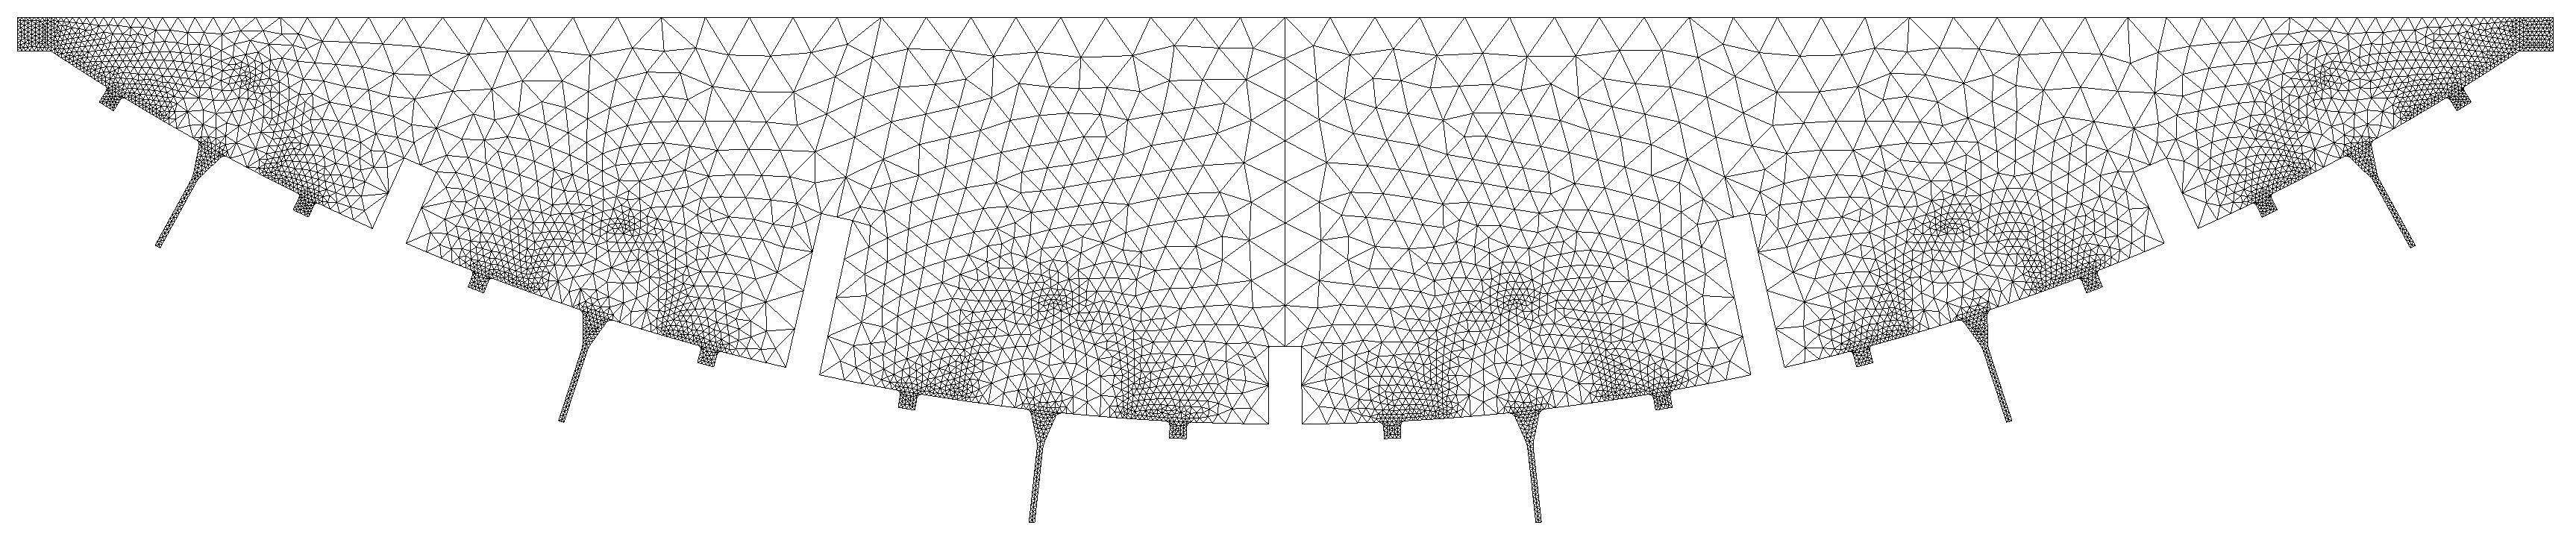
\includegraphics[width=\textwidth]{diagrams/meshes/inverted-circle-slice-6-flat_normal-walls.png}
                \caption{Diagram illustrates an example 2D mesh using triangular elements.}
                \label{fig:mesh-discretisation}
            \end{centering}
        \end{figure}

        As the name suggests, DGFEMs admit discontinuities in the approximation of the PDE solution. Following \cite{cangianiHpVersionDiscontinuousGalerkin2017}, we introduce the notation to describe averages and jumps between adjacent faces --- in this context, faces correspond to the $(d-1)$-dimensional boundaries of each $d$-dimensional element. There are two types of faces: interior faces and boundary faces; we write $\mathcal{F}^\mathcal{I}$ to denote interior faces between two elements, and $\mathcal{F}^\mathcal{B}$ to denote exterior (boundary) faces that lie on $\Gamma \equiv \partial \Omega$. We set $\mathcal{F} := \mathcal{F}^\mathcal{B} \cup \mathcal{F}^\mathcal{I}$ and note that $\mathcal{F}^\mathcal{B} \cap \mathcal{F}^\mathcal{I} = \emptyset$.

        %\todoitemthree{For viva: make sure you're familiar with trace operator}
        For matrix, vector, and scalar quantities (respectively, $\mat{A}$, $\vec{u}$, and $p$), the average operator defined on an interior face $F = \bar{\kappa}^+ \cap \bar{\kappa}^- \in \mathcal{F}^\mathcal{I}$ between two elements $\kappa^+, \kappa^- \in \mathcal{T}_h$, is given by
        \begin{align*}
            \begin{split}
                \averagevec{\mat{A}} & := \frac{1}{2} (\mat{A}^+ + \mat{A}^-),
            \end{split}\\
            \begin{split}
                \average{\vec{u}} & := \frac{1}{2} (\vec{u}^+ + \vec{u}^-),
            \end{split}\\
            \begin{split}
                \average{p} & := \frac{1}{2} (p^+ + p^-),
            \end{split}
        \end{align*}
        where $\cdot^\pm$ denote the trace values of $\mat{A}$, $\vec{u}$ and $p$ from inside element $\kappa^\pm$. We may similarly introduce the jump operator for vectors and scalars on an interior face, $F \in \mathcal{F}^\mathcal{I}$, as
        \begin{align*}
            \begin{split}
                \jumpvec{\vec{u}} & := \vec{u}^+ \otimes \vec{n}_{\kappa^+} + \vec{u}^- \otimes \vec{n}_{\kappa^-},
            \end{split}\\
            \begin{split}
                \jump{\vec{u}} & := \vec{u}^+ \cdot \vec{n}_{\kappa^+} + \vec{u}^- \cdot \vec{n}_{\kappa^-},
            \end{split}\\
            \begin{split}
                \jump{p} & := p^+ \vec{n}_{\kappa^+} + p^- \vec{n}_{\kappa^-},
            \end{split}
        \end{align*}
        where $\vec{n}_{\kappa^+}$ and $\vec{n}_{\kappa^-}$ denote the outward unit normals to $\kappa^+$ and $\kappa^-$, respectively, on $F$. Similarly, the average and jump operators on boundary faces, $F \in \mathcal{F}^\mathcal{B}$, where $F \subset \partial \kappa^+$, are defined as
        \begin{align*}
            \begin{split}
                \averagevec{\mat{A}} & := \mat{A}^+,
            \end{split}\\
            \begin{split}
                \average{\vec{u}} & := \vec{u}^+,
            \end{split}\\
            \begin{split}
                \average{p} & := p^+,
            \end{split}\\
            \begin{split}
                \jumpvec{\vec{u}} & := \vec{u}^+ \otimes \vec{n}_{\kappa^+},
            \end{split}\\
            \begin{split}
                \jump{\vec{u}} & := \vec{u}^+ \cdot \vec{n}_{\kappa^+},
            \end{split}\\
            \begin{split}
                \jump{p} & := p^+ \vec{n}_{\kappa^+}.
            \end{split}
        \end{align*}
    
        For all simulations in this thesis, we implement our DGFEM solver using AptoFEM \cite{houstonAptoFEMUserManual2024}, which is a general-purpose finite element method software package written in Fortran that permits DGFEM spaces, and interfaces to extremely fast third party matrix-solving packages such as MUMPS \cite{amestoyFullyAsynchronousMultifrontal2001}. Nonlinear equations are solved using a Newton solver, and linear equations are solved directly by MUMPS. Meshes are generated using Gmsh \cite{geuzaineGmshFiniteElement2009}, and solution data is visualised in ParaView \cite{ayachitParaViewGuideUpdated2015} and Matplotlib \cite{hunterMatplotlib2DGraphics2007}.

    \section{Equation discretisations} \label{sec:numerical-methods:equation-discretisations}    
        %\todoitemone{Before submission: check these discretisations again carefully.}
    
        In Chapter \ref{sec:modelling}, we introduced several PDEs describing fluid flow and oxygen transport. We will now discretise these equations using DGFEM in space and a first-order backward Euler scheme in time for simplicity.

        \subsection{Navier-Stokes-Darcy discretisation} \label{sec:numerical-methods:equation-discretisations:nsd}
            Here we detail the numerical discretisation for NSD, given in Equation \eqref{eq:nsb}. Discretisations for the alternative flow models given in Equations \eqref{eq:s-b}--\eqref{eq:ns-nsb} can be calculated through simple modifications of the appropriate coefficients for the following discretisation. For the spatial discretisation, we use a DGFEM together with a Lax-Friedrichs numerical flux approximation for the nonlinear convection term, following work undertaken by \citeauthor{cliffeAdaptiveDiscontinuousGalerkin2010} \cite{cliffeAdaptiveDiscontinuousGalerkin2010}. 

            \todoitemone{Need to define v explicitly in text? Not sure what this means.}
            Firstly, we make some definitions to ease the writing of the discretisations. Following a similar procedure to \cite{cockburnLocallyConservativeLDG2004,cliffeAdaptiveDiscontinuousGalerkin2010,gianiGoalorientedAdaptiveComposite2014}, we define two bilinear forms:
            \begin{align}
                \begin{split}
                    A_\text{f}(\vec{u}, \vec{v}) & := \mu \int_\Omega \nablab \vec{u} : \nablab \vec{v} \diff\vec{x} - \mu \int_{\mathcal{F}^\mathcal{I} \cup \Gamma_\text{f,D}} (\average{\nablab \vec{v}} : \jumpvec{\vec{u}} + \average{\nablab \vec{u}} : \jumpvec{\vec{v}}) \diff s \\ & + \mu \int_{\mathcal{F}^\mathcal{I} \cup \Gamma_\text{f,D}} \sigma \jumpvec{\vec{u}} : \jumpvec{\vec{v}} \diff s,
                \end{split}\\
                \begin{split}
                    B_\text{f}(\vec{v}, q) & := -\int_\Omega q \nablab \cdot \vec{v} \diff\vec{x} + \int_{\mathcal{F}^\mathcal{I} \cup \Gamma_\text{f,D}} \average{q} \jump{\vec{v}} \diff s,
                \end{split}
            \end{align}
            where $\Gamma_\text{f,D}, \Gamma_\text{f,N} \subseteq \mathcal{F}^\mathcal{B}$ denote the boundary faces on the Dirichlet and Neumann boundaries, respectively, $\vec{u}, \vec{v} \in \vec{V}_h$, $p, q \in Q_h$, $\sigma$ is the DGFEM symmetric interior penalty parameter, and $\nablab$ denotes the broken gradient operator: the usual gradient operator, $\nabla$, defined element-wise. We note that in the finite element context, $\vec{u}$ and $\vec{v}$ respectively correspond to the so-called trial and test functions in the space of $\vec{V}_h$. We define $|\kappa|$ to denote the area of an element, and $|F|$ to denote the length of a face. For the triangular meshes we are working with in this thesis, we select $\sigma = 10 \frac{r^2}{h}$ \cite{cangianiHpVersionDiscontinuousGalerkin2017, houstonEnergyNormShape2005, houstonAutomaticSymbolicComputation2018}, computed locally on a face with total degree $r$ and mesh width $h$, which for $F \in \mathcal{F}^\mathcal{I}$ is calculated as
            \begin{equation*}
                h|_F := \min \left( \frac{|\kappa^+|}{h^+_\perp}, \frac{|\kappa^-|}{h^-_\perp} \right),
            \end{equation*}
            and for $F \in \mathcal{F}^\mathcal{B}$ is calculated as
            \begin{equation*}
                h|_F := \frac{|\kappa^+|}{h^+_\perp},
            \end{equation*}
            where
            \begin{equation*}
                h^\pm_\perp := \frac{|\kappa^\pm|}{|F|},
            \end{equation*}
            and $\kappa^+$ and $\kappa^-$ are the neighbouring elements to the face. Loosely speaking, $h_\perp$ can be thought of as the orthogonal distance from a face to the opposite mesh vertex.

            We must also introduce a semilinear form that approximates the nonlinear advection term that appears in Equations \eqref{eq:navier-stokes} and \eqref{eq:navier-stokes-darcy}. We firstly introduce the function
            \begin{equation}
                \vec{u}_\Gamma := 
                \begin{cases}
                    \vec{u}^- & \text{on~} \mathcal{F}^\mathcal{I}, \\
                    \vec{u}^+ & \text{on~} \Gamma_\text{f,N}, \\
                    \vec{g}_\text{f,D} & \text{on~} \Gamma_\text{f,D}.
                \end{cases}
                \label{eq:u_gamma}
            \end{equation}
            We now introduce the Lax-Friedrichs flux for $F \in \mathcal{F}$ given by
            \begin{equation}
                \mathcal{H}_\text{f}(\vec{u}^+, \vec{u}_\Gamma, \vec{n})|_F := \frac{1}{2} ((\vec{u}^+ \otimes \vec{u}^+) \cdot \vec{n} + (\vec{u}_\Gamma \otimes \vec{u}_\Gamma) \cdot \vec{n} + \alpha(\vec{u}^+ - \vec{u}_\Gamma)),
                \label{eq:lax-friedrichs}
            \end{equation}
            where $\alpha := 2\max(|\vec{u}^+\cdot\vec{n}|, |\vec{u}_\Gamma\cdot\vec{n}|)$. Details regarding the derivation of $\alpha$ can be found in Appendix \ref{sec:lax-friedrichs}. The aforementioned semilinear form is then defined by
            \begin{multline}
                C_\text{f}(\vec{u}, \vec{v}) := - \rho \int_{\Omega} (\vec{u} \otimes \vec{u}) : \vec{\nabla}_h \vec{v} \diff \vec{x} + \rho \sum_{F \in \mathcal{F}} \int_{F} \mathcal{H}_\text{f}(\vec{u}^+, \vec{u}_\Gamma, \vec{n}_F) \cdot \vec{v}^+ \diff s \\ - \rho \sum_{F \in \mathcal{F}^\mathcal{I}} \int_{F} \mathcal{H}_\text{f}(\vec{u}^+, \vec{u}_\Gamma, \vec{n}_F) \cdot \vec{v}^- \diff s,
                \label{eq:nsb-wf-advection}
            \end{multline}
            where $\mathcal{F} \equiv \mathcal{F}^\mathcal{B} \cup \mathcal{F}^\mathcal{I}$ is the set of all faces, and $\vec{n}_F$ is the unit outward-pointing normal on a face $F$.
    
            A simple bilinear form is also introduced for the reaction term:
            \begin{equation}
                M_\text{f}(\vec{u}, \vec{v}) := \frac{\mu}{k} \int_\Omega \Psi ~ \vec{u} \cdot \vec{v} \diff \vec{x}.
            \end{equation}
    
            We finally define the following functionals for imposing the forcing function and boundary conditions:
            \begin{multline}
                    F_{\text{f},\vec{g}_\text{f,D}, \vec{g}_\text{f,N}}(\vec{v}) := \int_{\Omega} \vec{f}_\text{f} \cdot \vec{v} \diff\vec{x} - \int_{\Gamma_\text{f,N}} \vec{g}_\text{f,N}  \cdot\vec{v} \diff s + \int_{\Gamma_\text{f,D}} (\vec{g}_\text{f,D} \otimes \vec{n}) : \nablab \vec{v} \diff s \\ + \sigma\int_{\Gamma_\text{f,D}} \vec{v} \cdot \vec{g}_\text{f,D} \diff s,
            \end{multline}
            \begin{equation}
                    G_{\text{f},\vec{g}_\text{f,D}}(q) := \int_{\Gamma_\text{f,D}} q ~ \vec{g}_\text{f,D} \cdot \vec{n} \diff s.
            \end{equation}

            The \textit{steady-state} (i.e., $\pdv{\vec{u}}{t} \equiv \vec{0}$) Navier-Stokes-Darcy discretisation is then given by: find $(\vec{u}_h, p_h) \in (\vec{V}_h, Q_h)$ such that
            \begin{multline}
                \overbrace{A_\text{f}(\vec{u}_h, \vec{v}_h)}^{\text{diffusion}} + \overbrace{C_\text{f}(\vec{u}_h, \vec{v}_h)}^{\text{advection}} + \overbrace{M_\text{f}(\vec{u}_h, \vec{v}_h)}^{\text{reaction}} + \overbrace{B_\text{f}(\vec{v}_h, p_h)}^{\text{pressure}} - \overbrace{B_\text{f}(\vec{u}_h, q_h)}^{\text{incompressibility}} \\ = \overbrace{F_{\text{f},\vec{g}_\text{f,D},\vec{g}_\text{f,N}}(\vec{v}_h) - G_{\text{f},\vec{g}_\text{f,D}}(q_h)}^{\text{forcing and boundary conditions}},
                \label{eq:nsb-discretisation}
            \end{multline}
            for all $(\vec{v}_h, q_h) \in (\vec{V}_h, Q_h)$. The label on each term shows how each term in the discretisation relates back to the original PDE. We note here that the boundary conditions are applied weakly, in which the approximate solution is not required to satisfy the boundary conditions exactly, and instead enforces the boundary conditions through additional terms in the discretisation \cite{bazilevsWeakImpositionDirichlet2007}.

            For the \textit{time-dependent} Navier-Stokes-Darcy discretisation, we first state the weak formulation of the momentum equation in the form:
            \begin{equation}
                \rho \int_\Omega \pdv{\vec{u}}{t} \cdot \vec{v} \diff\vec{x} = \int_\Omega \mathcal{L}(\vec{u}, p) \cdot \vec{v} \diff \vec{x},
                \label{eq:nsb-wf-time-with-operator}
            \end{equation}
            where $\mathcal{L}$ is the spatial differential operator for all terms beside the time derivative of the momentum equation for NSD, given in Equation \eqref{eq:nsb:momentum}. We define the following bilinear form for this term:
            \begin{equation}
                L_\text{f}(\vec{u}, \vec{v}) := \rho \int_{\Omega} \pdv{\vec{u}}{t} \cdot \vec{v} \diff\vec{x}.
                \label{eq:nsb-wf-time}
            \end{equation}%
            Assuming the RHS of Equation \eqref{eq:nsb-wf-time-with-operator} is discretised in space as presented in Equation \eqref{eq:nsb-discretisation}, we have a choice on how the time derivative is discretised. As is generally standard in the FEM literature, we discretise the time derivative term using a finite difference method, and for simplicity use a simple first-order backward Euler approximation. For uniform time-stepping, this involves choosing a constant step size $\Delta t$, which defines the distance between subsequent approximations at times $\{ t^0 + n \Delta t \, | \, n \in \{0, 1, 2, ...\} \}$, where $t^0$ is the initial time. The backward Euler method is derived from making an approximation of the form:
            \begin{equation}
                \pdv{\vec{u}^{n+1}}{t} \approx \frac{\vec{u}^{n+1} - \vec{u}^n}{\Delta t},
                \label{eq:first-order-backward-euler}
            \end{equation}
            and approximating the right-hand side of Equation \eqref{eq:nsb-wf-time-with-operator} at time $t^{n+1}$, where $\{ \vec{u}^n \, | \, n \in \{ 0, 1, 2, ... \} \}$ are subsequent approximations of $\vec{u}$ in time. For our problem, this equates to:
            \begin{equation*}
                \rho \int_\Omega \frac{(\vec{u}^{n+1} - \vec{u}^n) \cdot \vec{v}}{\Delta t} \diff \vec{x} = \int_\Omega \mathcal{L}(\vec{u}^{n+1}, p^{n+1}) \cdot \vec{v} \diff \vec{x}.
            \end{equation*}
            We introduce an additional bilinear form definition to make use of this approximation:
            \begin{equation}
                E_\text{f}(\vec{u}, \vec{v}) := \frac{\rho}{\Delta t} \int_\Omega \vec{u} \cdot \vec{v} \diff \vec{x}.
                \label{eq:nsb-wf-time-euler}
            \end{equation}
            The \textit{time-dependent} Navier-Stokes-Darcy discretisation is then given by: find $(\vec{u}^{n+1}_h, p^{n+1}_h) \in (\vec{V}_h, Q_h)$ such that
            \begin{multline}
                \overbrace{E_\text{f}(\vec{u}^{n+1}_h, \vec{v}_h) - E_\text{f}(\vec{u}^n_h, \vec{v}_h)}^{\text{time}} + \overbrace{A_\text{f}(\vec{u}^{n+1}_h, \vec{v}_h)}^{\text{diffusion}} + \overbrace{C_\text{f}(\vec{u}^{n+1}_h, \vec{v}_h)}^{\text{advection}} + \overbrace{M_\text{f}(\vec{u}^{n+1}_h, \vec{v}_h)}^{\text{reaction}} + \\ \overbrace{B_\text{f}(\vec{v}_h, p^{n+1}_h)}^{\text{pressure}} - \overbrace{B_\text{f}(\vec{u}^{n+1}_h, q_h)}^{\text{incompressibility}} = \overbrace{F_{\text{f},\vec{g}_\text{f,D},\vec{g}_\text{f,N}}(\vec{v}_h) - G_{\text{f},\vec{g}_\text{f,D}}(q_h)}^{\text{forcing and boundary conditions}},
                \label{eq:nsb-discretisation-time}
            \end{multline}
            for all $(\vec{v}_h, q_h) \in (\vec{V}_h, Q_h)$, given the DGFEM approximation of the velocity at the previous time-step, $\vec{u}^n_h \in \vec{V}_h$, $n \in \{0, 1, 2, ...\}$, including an initial condition of $\vec{u}^0_h$. For the time-dependent simulations presented later in this thesis, we obtain $\vec{u}^0_h$ from the steady-state Navier-Stokes-Darcy discretisation presented in Equation \eqref{eq:nsb-discretisation}.

            %\todoitemthree{Note: you'll probably be asked about this in the viva.}
            Discretisations for the other blood flow models can be written by simple modification of the coefficients on each term of the NSD discretisation.

        \subsection{Reaction-advection-diffusion discretisation} \label{sec:numerical-methods:equation-discretisations:rad}
            The discretisation for the reaction-advection-diffusion equation given in Equation \eqref{eq:rad} is similar to the one given above for the velocity approximation. In particular, we will again use a DGFEM for the spatial discretisation. The main difference with the oxygen transport model is that the convection term is linear, as $\vec{u}$ is known a priori due to a one-way coupling between the blood velocity and oxygen transport models.

            Similar to the definition of $A_\text{f}$ for the velocity model discretisation, we follow work by \citeauthor{cangianiHpVersionDiscontinuousGalerkin2017} \cite{cangianiHpVersionDiscontinuousGalerkin2017} and define
            \begin{multline}
                A_\text{c}(c, \eta) := D \int_\Omega \nablab c \cdot \nablab \eta \diff\vec{x} - D \int_{\mathcal{F}^\mathcal{I} \cup \Gamma_\text{c,D}} (\average{\nablab c} \cdot \jump{\eta} + \average{\nablab \eta} \cdot \jump{c}) \diff s \\ + D \int_{\mathcal{F}^\mathcal{I} \cup \Gamma_\text{c,D}} \sigma \jump{c} \cdot \jump{\eta} \diff s,
            \end{multline}
            where we again select $\sigma = 10 \frac{s^2}{h}$ on a face with total degree $s$ and mesh width $h$, and $c, \eta \in C_h$, and $\Gamma_\text{c,D},\Gamma_\text{c,N} \subseteq \mathcal{F}^\mathcal{B}$ denote the boundary faces of the Dirichlet and Neumann boundaries, respectively, for the oxygen concentration problem.

            %\todoitemthree{Reference for $\alpha$ here?}
            The advection discretisation term for the reaction-advection-diffusion equation is simpler than that of the velocity model, as it is linear in $c$. We firstly introduce the function
            \begin{equation}
                c_\Gamma := 
                \begin{cases}
                    c^- & \text{on~} \mathcal{F}^\mathcal{I}, \\
                    c^+ & \text{on~} \Gamma_\text{c,N}, \\
                    g_\text{c,D} & \text{on~} \Gamma_\text{c,D}.
                \end{cases}
                \label{eq:c_gamma}
            \end{equation}
            We also introduce the Lax-Friedrichs flux for $F \in \mathcal{F}$ by
            \begin{equation}
                \mathcal{H}_\text{c}(c^+, c_\Gamma, \vec{n})|_F := \frac{1}{2}((\vec{u}^+ \cdot \vec{n}) c^+ + (\vec{u}^- \cdot \vec{n}) c_\Gamma + \alpha(c^+ - c_\Gamma)),
            \end{equation}
            where $\alpha := |\average{\vec{u}} \cdot \vec{n}|$. The bilinear form for this advection term is then given by
            \begin{multline}
                C_\text{c}(c, \eta; \vec{u}) := -\int_\Omega c ~ \vec{u} \cdot \vec{\nabla}_h \eta \diff \vec{x} + \sum_{F \in \mathcal{F}} \int_F \mathcal{H}_\text{c}(c^+, c_\Gamma, \vec{n}_F)\eta^+ \diff s \\ - \sum_{F \in \mathcal{F}^\mathcal{I}} \int_F \mathcal{H}_\text{c}(c^+, c_\Gamma, \vec{n}_F)\eta^- \diff s.
            \end{multline}            

            Two simple bilinear forms must also be introduced for the reaction and time terms, respectively given as:
            \begin{equation}
                M_\text{c}(c, \eta) := R \int_\Omega \Psi ~ c ~ \eta \diff \vec{x},
            \end{equation}
            \begin{equation}
                L_\text{c}(c, \eta) := \int_\Omega \pdv{c}{t} ~ \eta \diff \vec{x}.
                \label{eq:rad-wf-time}
            \end{equation}
            We once again employ a simple first-order backward Euler approximation of the time derivative, which is used by defining:
            \begin{equation}
                E_\text{c}(c, \eta) := \frac{1}{\Delta t} \int_\Omega c ~ \eta \diff \vec{x}.
                \label{eq:rad-wf-time-euler}
            \end{equation}
    
            We finally define the following functional for imposing the boundary conditions:
            \begin{multline}
                F_{\text{c},g_\text{c,D}, g_\text{c,N}}(\eta) := \int_\Omega f_\text{c} \eta \diff\vec{x} - \int_{\Gamma_\text{c,N}} g_\text{c,N} ~ \eta \diff s + \int_{\Gamma_\text{f,D}} g_\text{c,D} ~ (\nablab \eta \cdot \vec{n}) \diff s \\ + \sigma\int_{\Gamma_\text{c,D}} g_\text{c,D} ~ \eta \diff s.
            \end{multline}           
            
            The \textit{time-dependent} reaction-advection-diffusion equation is given by: find $c^{n+1}_h \in C_h$ such that
            \begin{multline}
                \overbrace{E_\text{c}(c^{n+1}_h, \eta_h) - E_\text{c}(c^n_h, \eta_h)}^{\text{time}} + \overbrace{A_\text{c}(c^{n+1}_h, \eta_h)}^{\text{diffusion}} + \overbrace{C_\text{c}(c^{n+1}_h, \eta_h; \vec{u}^{n+1}_h)}^{\text{advection}} + \overbrace{M_\text{c}(c^{n+1}_h, \eta_h)}^{\text{reaction}} \\ = \underbrace{F_{\text{c},g_\text{c,D},g_\text{c,N}}(\eta_h),}_{\text{forcing and boundary conditions}}
                \label{eq:rad-discretisation}
            \end{multline}
            for all $\eta_h \in C_h$, given $\vec{u}^{n+1}_h$, where $\vec{u}^{n+1}_h$ is the approximation to Equation \eqref{eq:nsb-discretisation} at time level $t^{n+1}$, given $c^n_h$, $n \in \{0, 1, 2, ...\}$, including an initial condition of $c^0_h$. We note that the \textit{steady-state} discretisation involves simply discarding the time terms given in Equation \eqref{eq:rad-discretisation}.

            We will now perform a convergence study through mesh refinement using the method of manufactured solutions in order to verify our implementation of these numerical methods.

    \section{Convergence to analytical solution} \label{sec:numerical-methods:convergence}
        Here, we will briefly test our code that implements the numerical discretisations of the Navier-Stokes-Darcy equation (Equation \eqref{eq:nsb}) and the reaction-advection-diffusion equation (Equation \eqref{eq:rad}) using the method of manufactured solution (MMS). We will show that we obtain optimal convergence rates through mesh and time-step refinement.

        MMS is one commonly employed method for verifying correct implementation of finite element code \cite{roacheCodeVerificationMethod2002}. The overarching aim of MMS is to select an analytical solution that solves the PDE that has been discretised, where this solution is of sufficient complexity to ensure that all derivatives are properly exercised. By taking the approximate solutions that arise from the discretisation, we may then measure an error between the exact and approximate solutions. By computing successively higher resolution approximations, we may study the behaviour of the error, for which there are typically so-called `a priori' error bounds that describe the rate at which the error should decrease.
        
        Our approach to this involves selecting an appropriate analytical solution for the velocity, pressure, and oxygen concentration fields ($\vec{u}$, $p$, $c$, respectively), then setting the forcing function equal to the residual of the PDE with these solutions. In order to test the discretisations in both space and time, we separately increase the resolution and study the corresponding convergence rates in the $L^2$-norm.

        %\todoitemtwo{Include $\Omega$ in definition of $L^2$-norm; requires updating the figure.}
        We specifically select analytical solutions on domain $\Omega$:
        \begin{subequations}
            \begin{alignat}{3}
                u_1 & := - && \cos(t)(y\cos(y) + \sin(y))\exp(x), \label{eq:analytical-solutions:u1}\\
                u_2 & := && \cos(t)y\sin(y)\exp(x), \label{eq:analytical-solutions:u2}\\
                p & := && \cos(t) 2 \exp(x) \sin(y), \label{eq:analytical-solutions:p}\\
                c & := && \cos(t) \exp(x - y), \label{eq:analytical-solutions:c}
            \end{alignat}%
            \label{eq:analytical-solutions}%
        \end{subequations}%
        where $\vec{u} \equiv (u_1, u_2)^\intercal$, and boundary conditions are appropriately selected. We then select forcing functions $\vec{f}_\text{f}$ and $f_\text{c}$ such that these analytical solutions solve the PDEs. Between each approximate and exact solution, we calculate $\norm{\vec{u} - \vec{u}_h}_{L^2}$, $\norm{p - p_h}_{L^2}$, and $\norm{c - c_h}_{L^2}$, where the $L^2$-norm over $\Omega$ is defined as
        \begin{equation}
            \norm{u}_{L^2} := \sqrt{\int_\Omega u^2 \diff \vec{x}}.
        \end{equation}
        For simplicity, in these tests we set all problem coefficients for Equations \eqref{eq:nsb} and \eqref{eq:rad} to unity, the final time $T = 1$, the time-step $\Delta t := 0.01$, and $\Omega := [0, 1]^2$. 

        For the numerical methods presented here, we expect spatial convergence rates in the $L^2$-norm between an exact and approximate solution of $\mathcal{O}(h^{p+1})$ \cite{cangianiHpVersionDiscontinuousGalerkin2017}, where $h$ is related to element widths and $p$ is the (fixed) polynomial degree of the space, and temporal convergence rates of $\mathcal{O}(\Delta t)$ due to the first-order time-stepping scheme. For the solution spaces we have chosen in Equation \eqref{eq:velocity-spaces} with $r = 2$ and $s = 1$, we therefore expect
        \begin{subequations}
            \begin{align}
                ||\vec{u} - \vec{u}_h||_{L^2} & = \mathcal{O}(h^3) + \mathcal{O}(\Delta t), \label{eq:convergence-rates:u}\\
                ||p - p_h||_{L^2} & = \mathcal{O}(h^2) + \mathcal{O}(\Delta t), \label{eq:convergence-rates:p}\\
                ||c - c_h||_{L^2} & = \mathcal{O}(h^2) + \mathcal{O}(\Delta t). \label{eq:convergence-rates:c}
            \end{align}
            \label{eq:convergence-rates}
        \end{subequations}
        Clearly, spatial or temporal errors may dominate depending upon the chosen discretisation parameters, so we select a small $\Delta t$ when investigating spatial convergence, and select a small $h$ when investigating temporal convergence.

        We use $N_\text{DoF}$ to denote the number of degrees of freedom associated with the Navier-Stokes-Darcy discretisation, which in 2D with fixed polynomial degrees is related to the mesh width by 
        \begin{equation*}
            N_\text{DoF} \propto h^{-2}.
        \end{equation*}
        Figures \ref{fig:mms-convergence:space} and \ref{fig:mms-convergence:time} respectively present the convergence rates under spatial and temporal refinement, which agree with the expected rates from Equation \eqref{eq:convergence-rates}.

        \begin{figure}
            % Generated 2024-04-25.
            %  File run: ./drivers/convergency.py.
            %  And to visualise: plot_from_data() in ./plotting/plot_convergence.py.
            \centering
            \begin{subfigure}{0.45\textwidth}
                \centering
                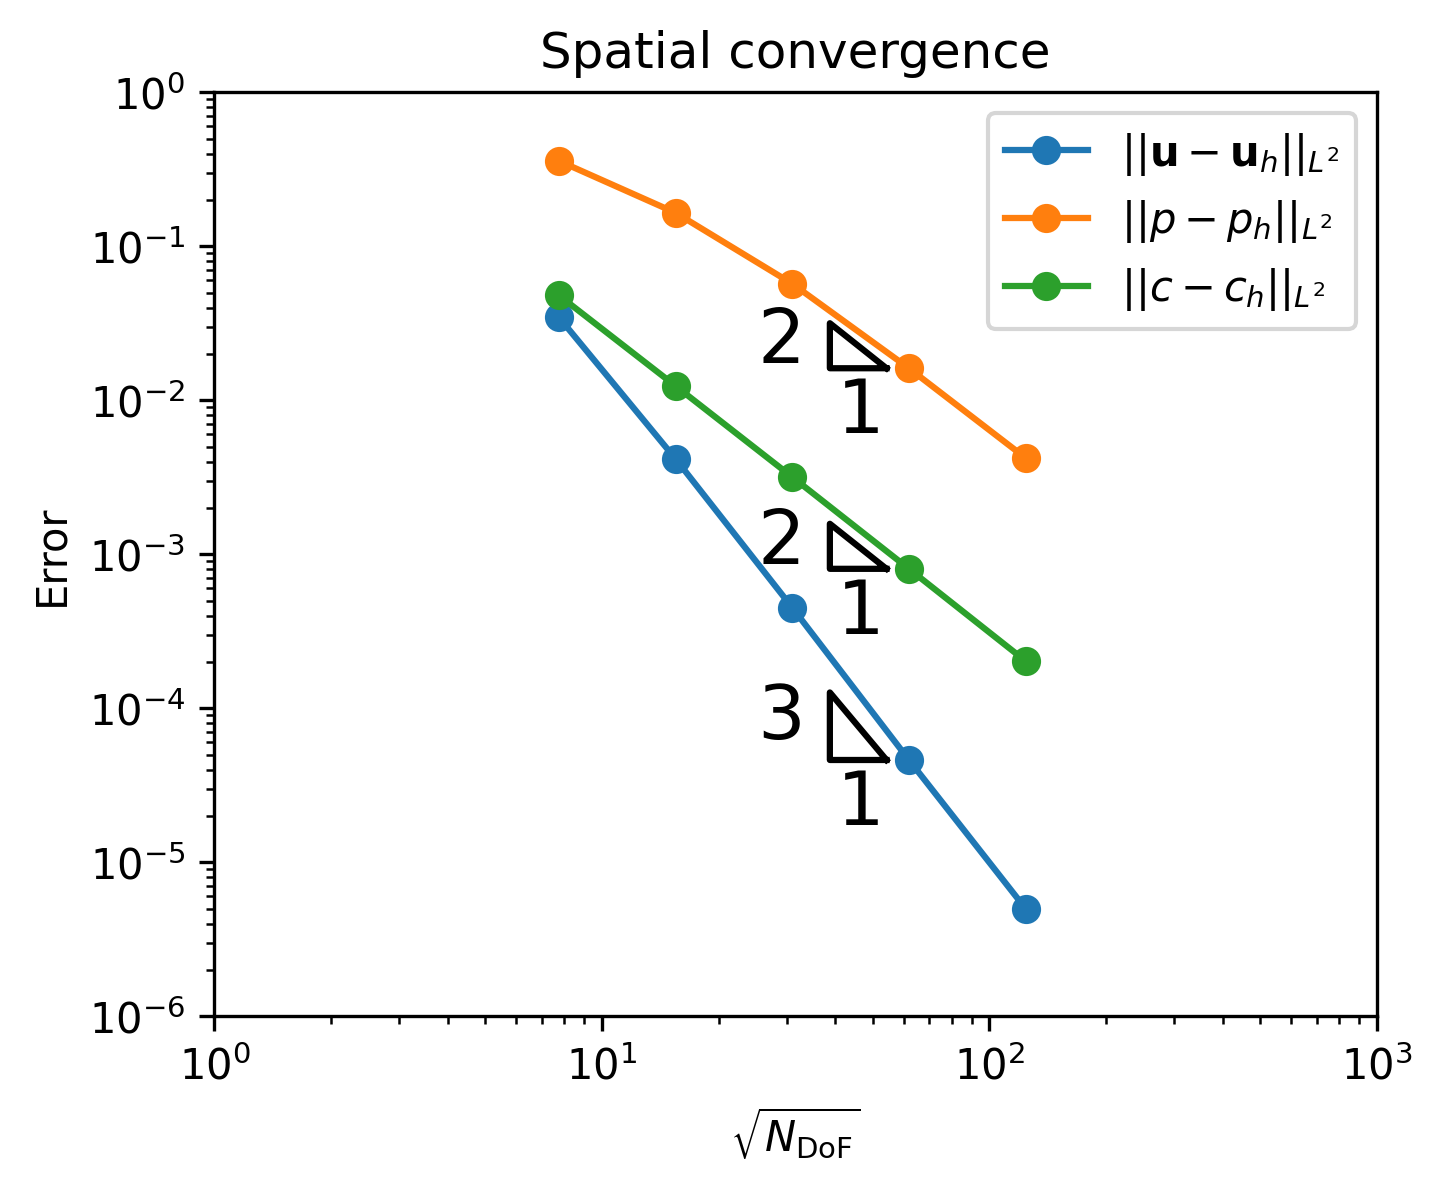
\includegraphics[width=\textwidth]{diagrams/results-convergence/spatial_convergence.png}
                \caption{}
                \label{fig:mms-convergence:space}
            \end{subfigure}
            \hfill
            \begin{subfigure}{0.45\textwidth}
                \centering
                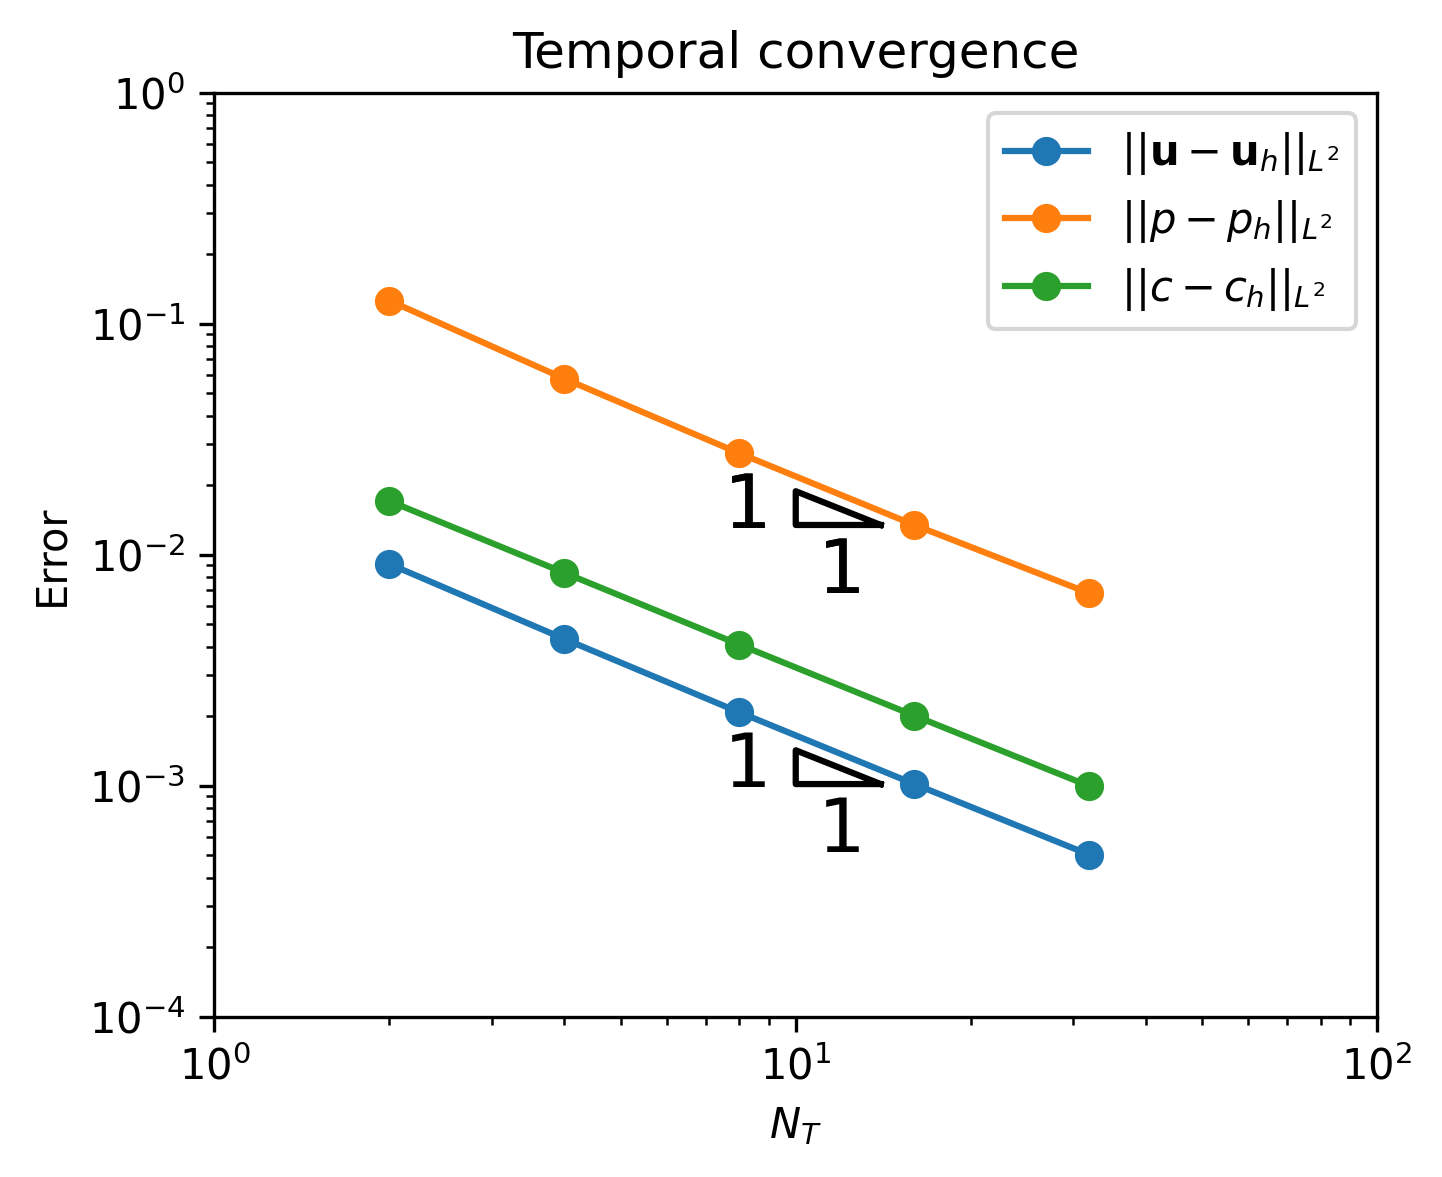
\includegraphics[width=\textwidth]{diagrams/results-convergence/temporal_convergence.png}
                \caption{}
                \label{fig:mms-convergence:time}
            \end{subfigure}
            \caption{Visualisations of the convergence rates of the tests outlined in \S\ref{sec:numerical-methods:convergence}. Graphs show (a) spatial convergence, and (b) temporal convergence of the velocity, pressure, and oxygen concentration fields.}
            \label{fig:mms-convergence}
        \end{figure}

        We will now present further numerical experiments on physical problems. For the remainder of the thesis, we will set $\vec{f}_\text{f} \equiv \vec{0}$ and $f_\text{c} \equiv 0$, except in Chapter \ref{sec:contractions} where we again use MMS.
    
    \section{Blood flow numerical experiments} \label{sec:numerical-methods:blood-flow-experiments}    
        One of the key contributions of this thesis is employing the Navier-Stokes-Darcy (NSD) equation for modelling maternal blood flow on a 2D whole-organ placenta geometry. \S\ref{sec:numerical-methods:blood-flow-experiments:comparison} will therefore present this model alongside two other common choices in the literature, highlighting the difference in behaviour between each model. \S\ref{sec:numerical-methods:blood-flow-experiments:asymmetric} will then present only the NSD flow model on a placenta geometry with vessels placed asymmetrically, which will be used as the basis of the investigations in Chapters \ref{sec:numerical-mri} and \ref{sec:contractions}.

        \subsection{Model comparison} \label{sec:numerical-methods:blood-flow-experiments:comparison}
            %\todoitemtwo{Include example meshes x2 (with zoom in?), plus numbers of DoFs}
        
            We select model parameters from Tables \ref{tab:structural-parameters} and \ref{tab:problem-parameters} and use the discretisations from \S\ref{sec:numerical-methods:equation-discretisations} to approximate solutions to the NSD model, as well as the two other models discussed in \S\ref{sec:modelling:blood-flow:s+b} and \S\ref{sec:modelling:blood-flow:ns+nsb}. For simplicity, we consider only the \textit{steady-state} versions ($\pdv{\vec{u}}{t} \equiv \vec{0}$) all three flow models, and assume that vessels in the placenta geometry are located only on the basal plate and appear symmetrically. We approximate solutions on both the placentone and placenta geometries. A side-by-side comparison is shown for the 2D placentone and 2D placenta geometries in Figures \ref{fig:4-models-placentone} and \ref{fig:4-models-placenta}, respectively.

            \begin{figure}
                \thisfloatpagestyle{empty}
                % GENERATED WITH MONOLITH COMMIT: XXX
                % GENERATED ON 2024-XX-XX
                \centering
                \begin{subfigure}[b]{0.45\textwidth}
                    \centering
                    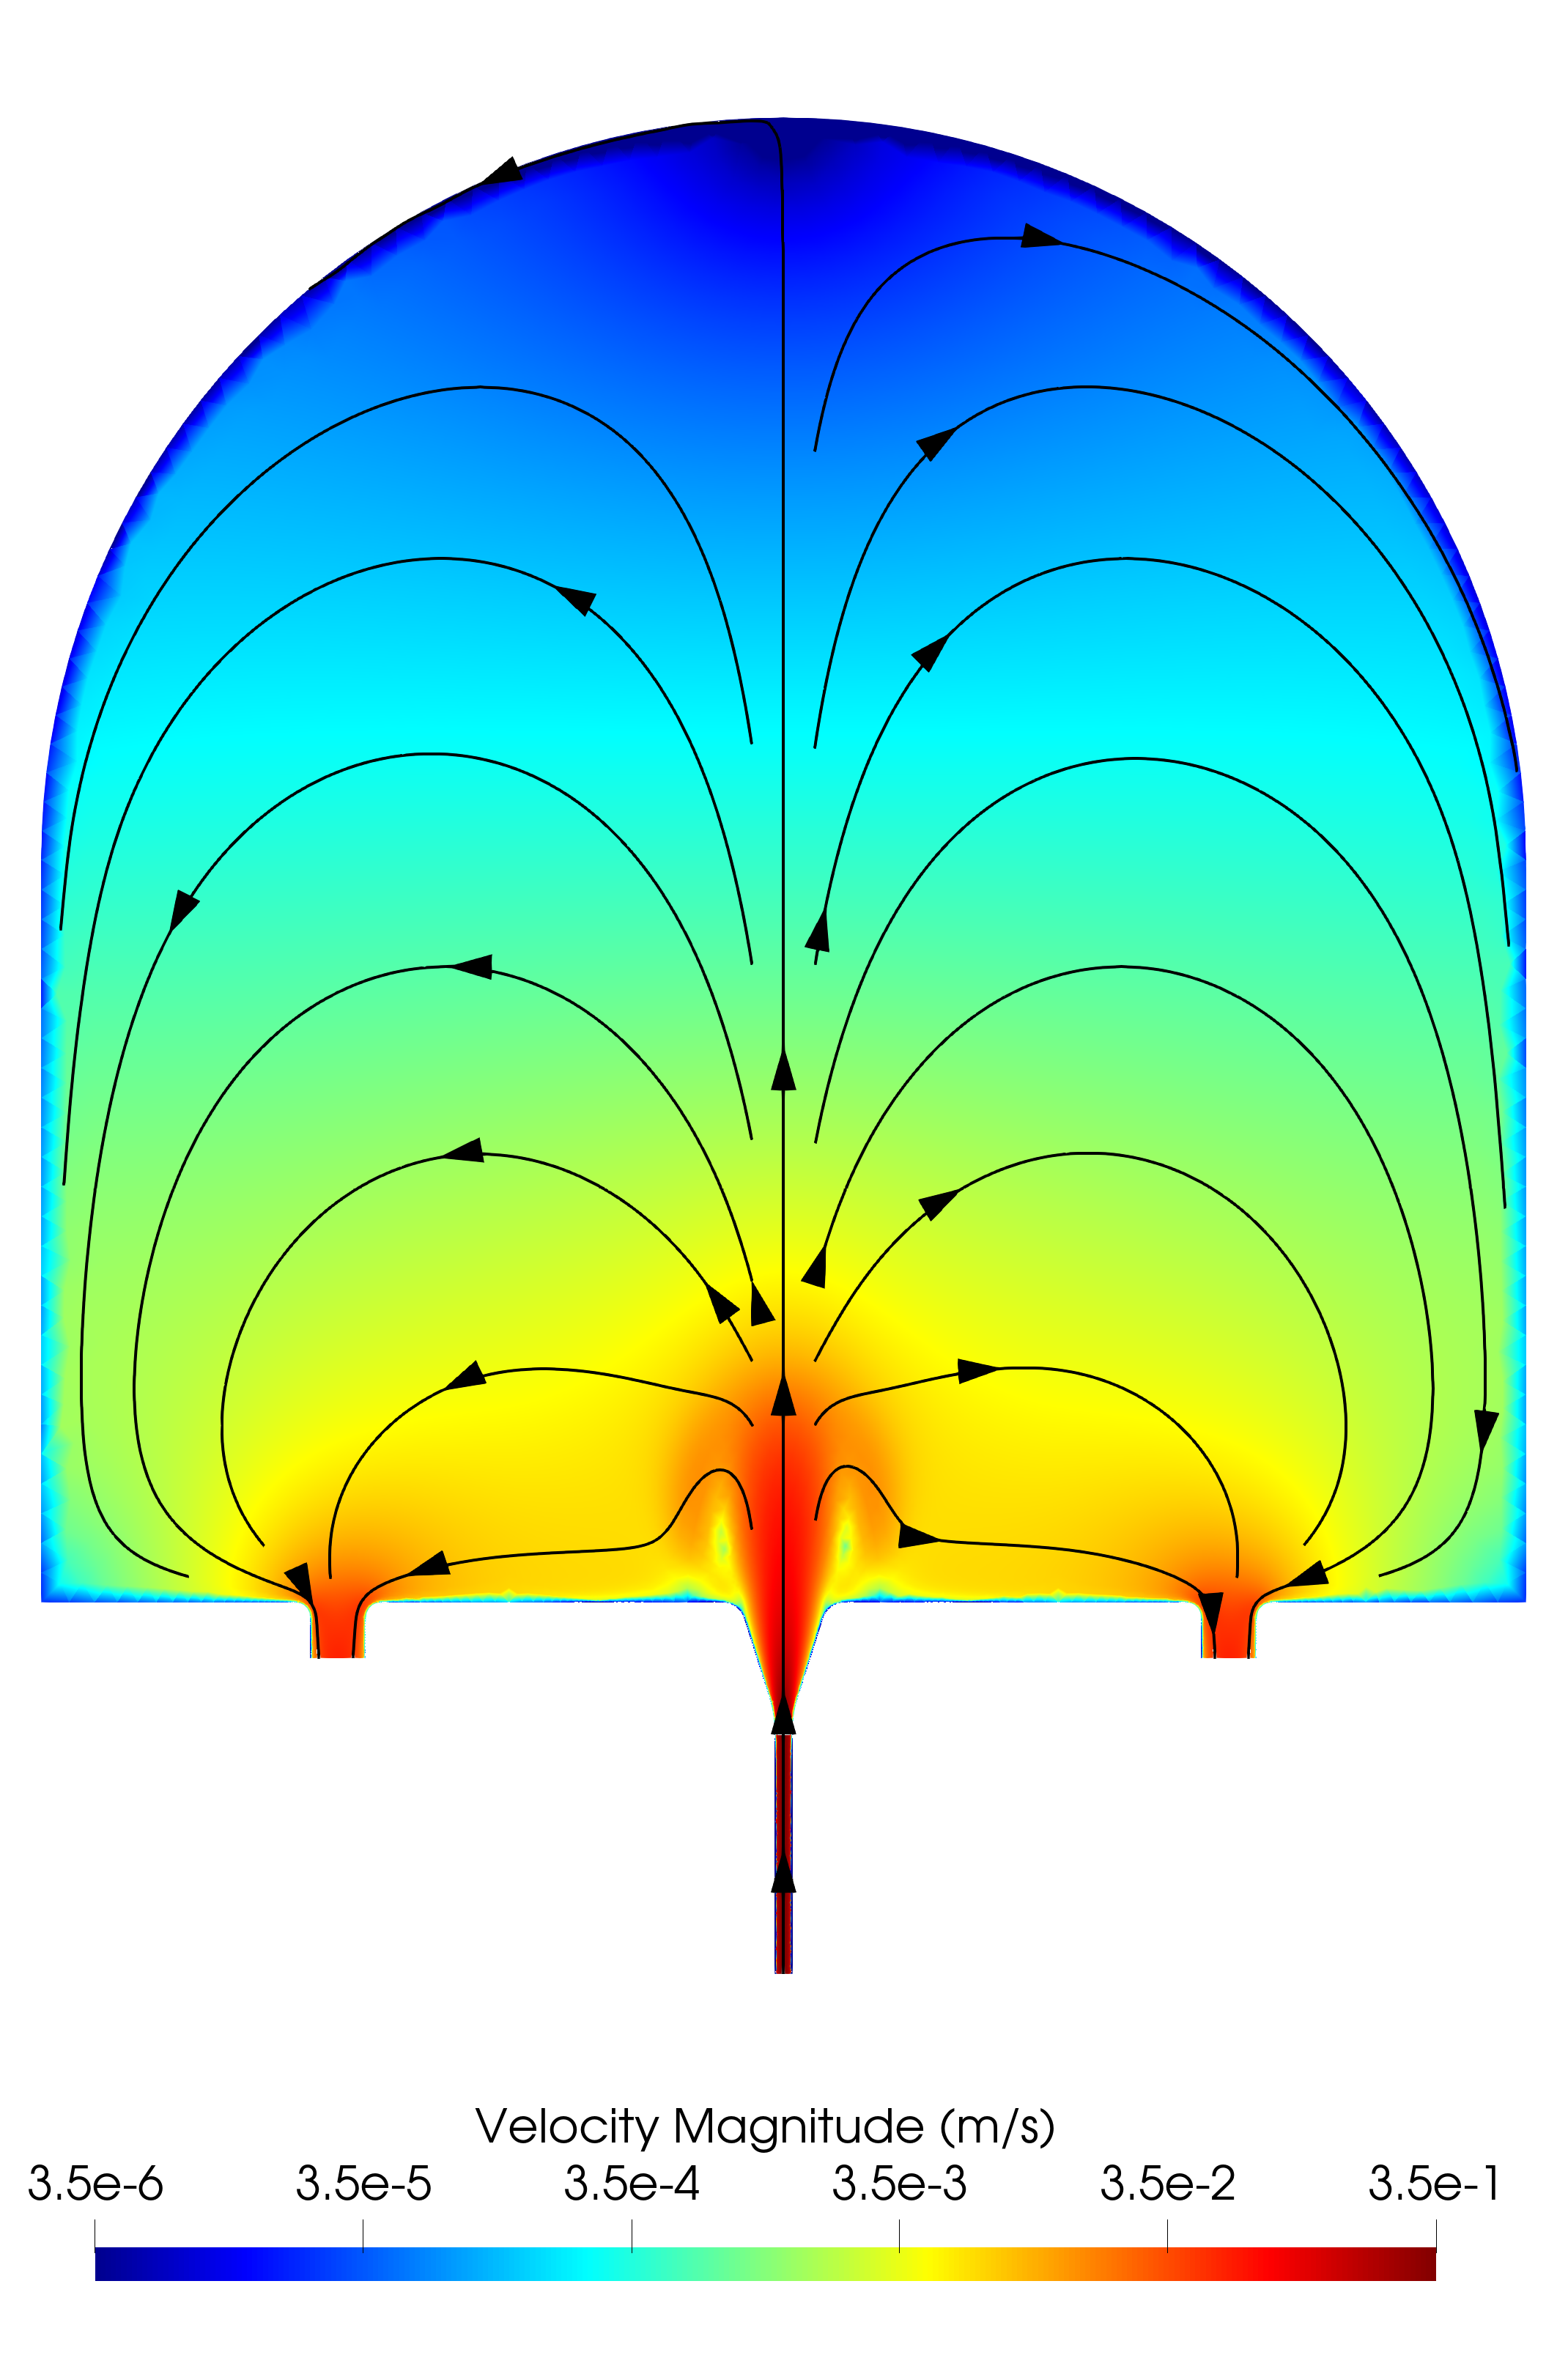
\includegraphics[width=\textwidth]{diagrams/results-modelling/velocity-transport/meshandsoln_dg_velocity_placentone_nsb_velocity-log.png}
                    \caption{}
                    \label{fig:4-models-placentone:nsb}
                \end{subfigure}
                \hfill
                \begin{subfigure}[b]{0.45\textwidth}
                    \centering
                    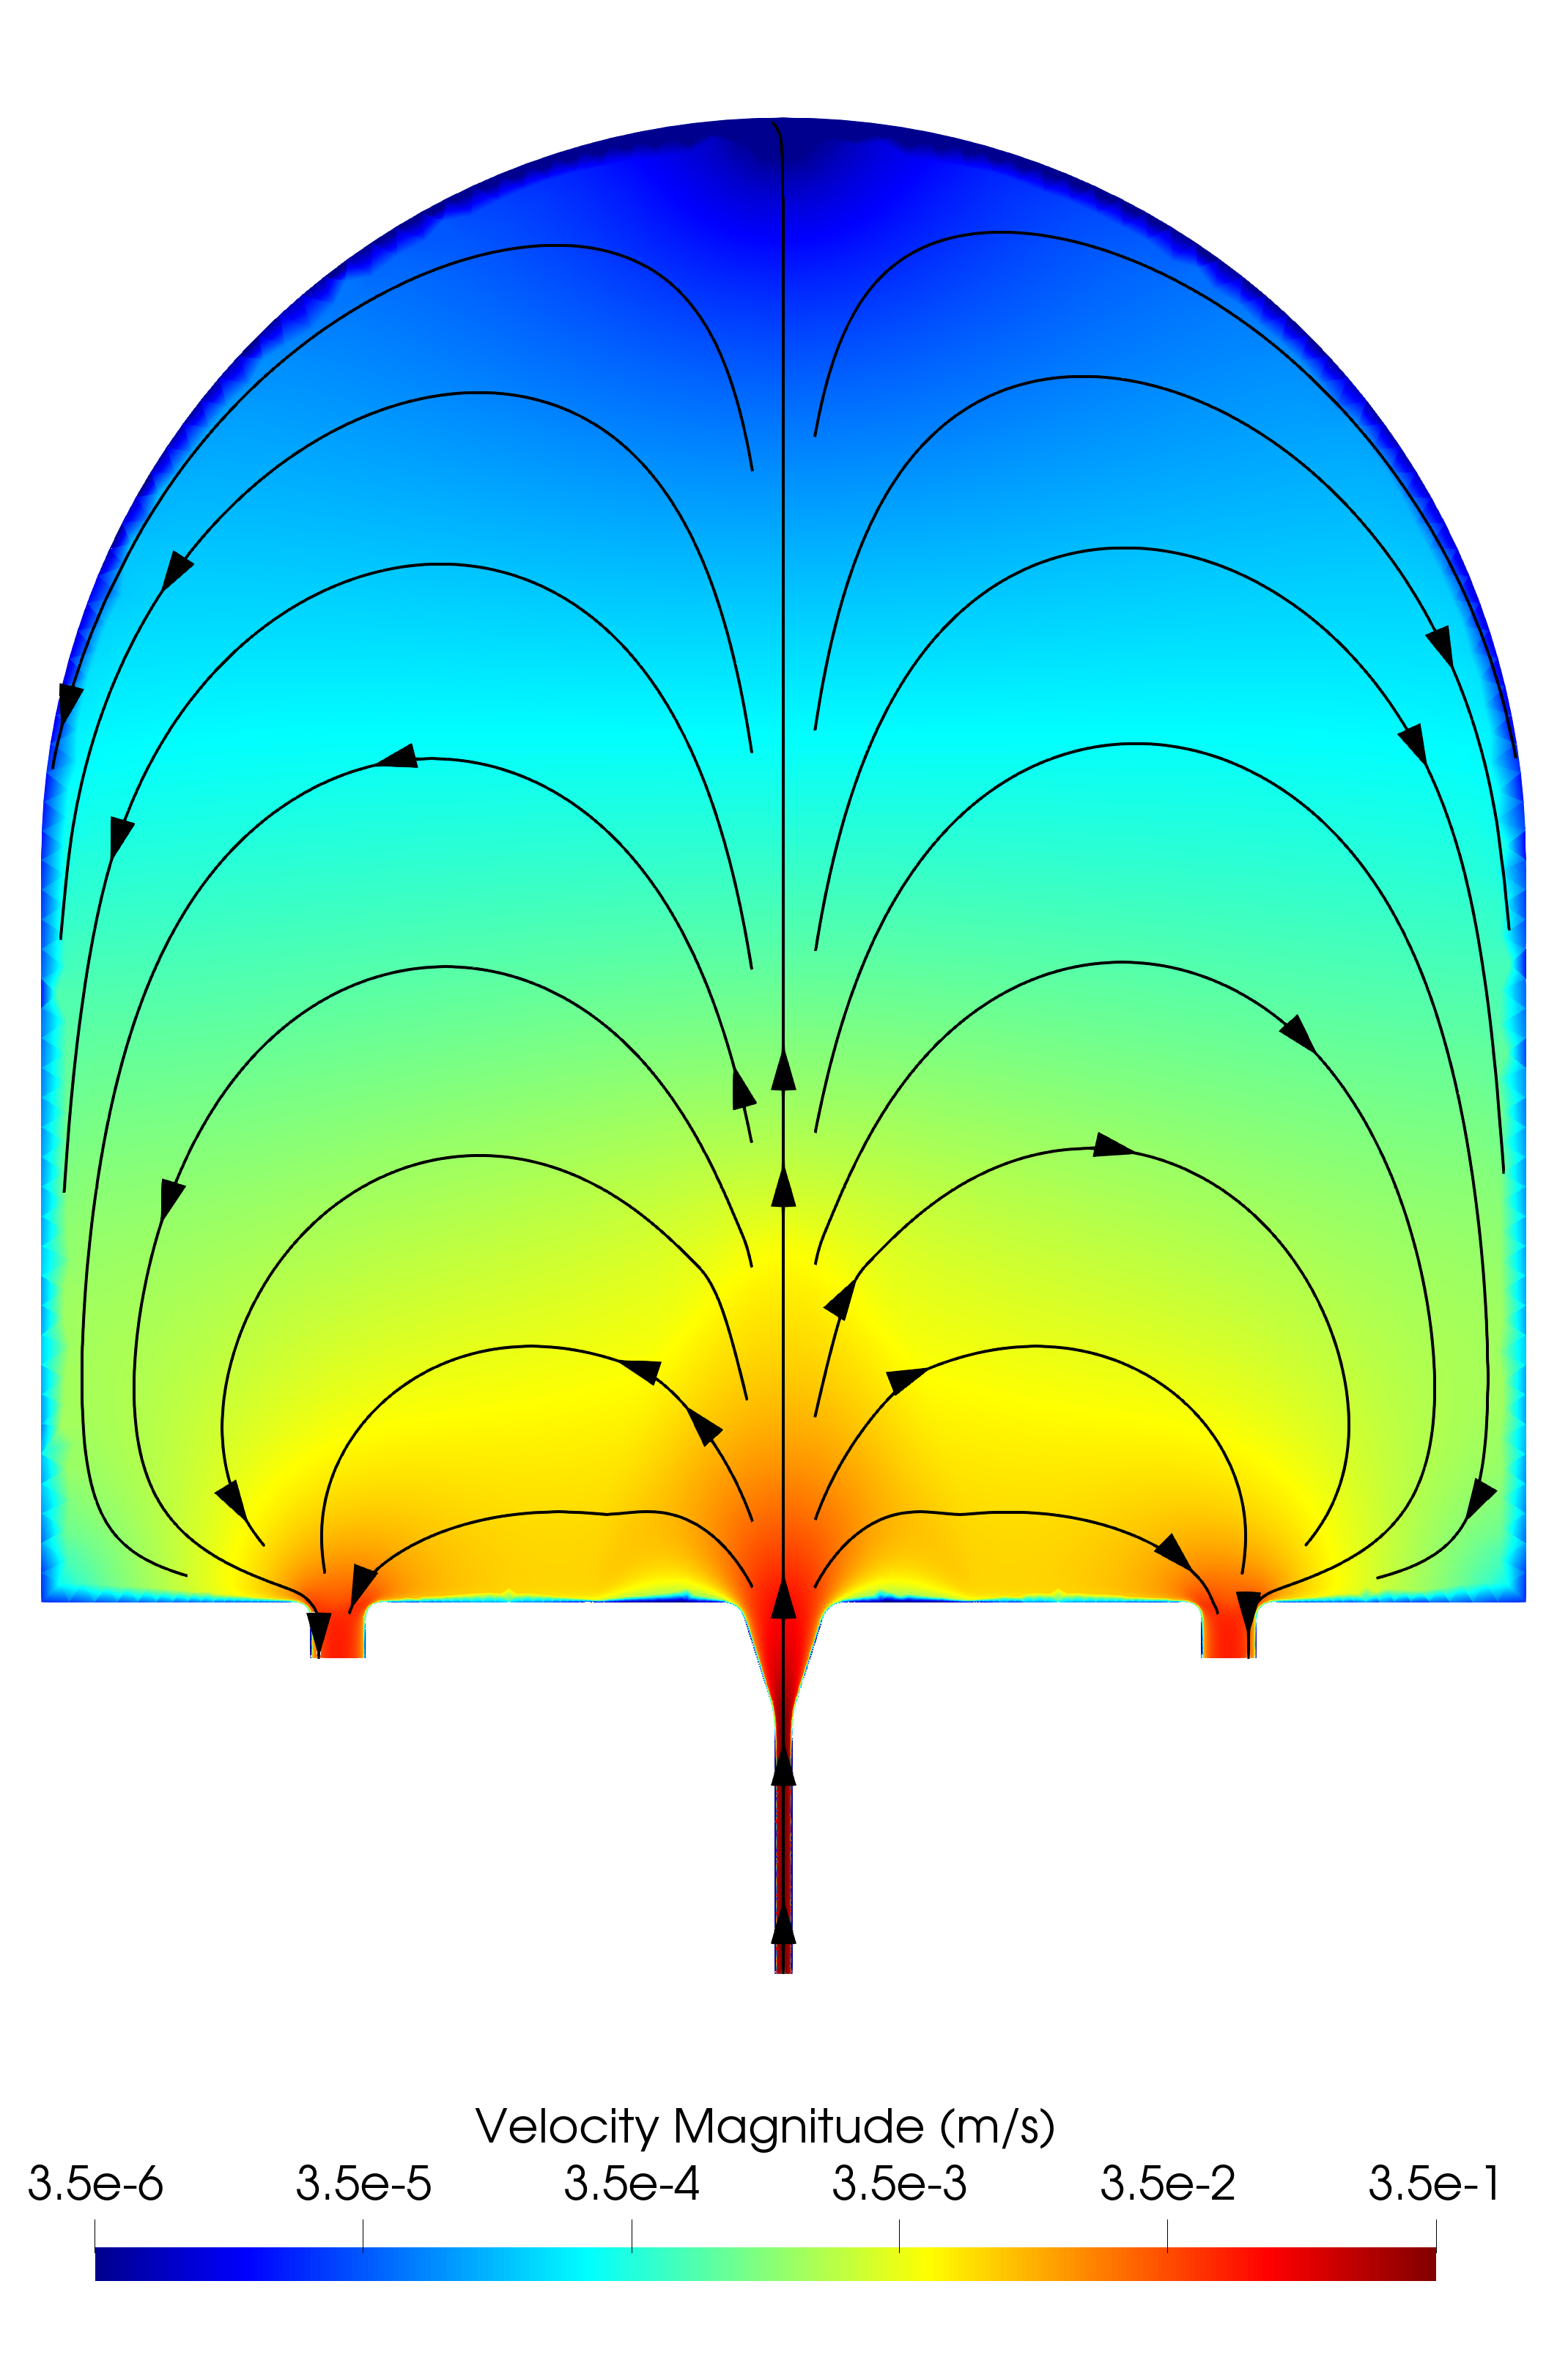
\includegraphics[width=\textwidth]{diagrams/results-modelling/velocity-transport/meshandsoln_dg_velocity_placentone_s-b_velocity-log.png}
                    \caption{}
                    \label{fig:4-models-placentone:s-b}
                \end{subfigure}
                \hfill
                \begin{subfigure}[b]{0.45\textwidth}
                    \centering
                    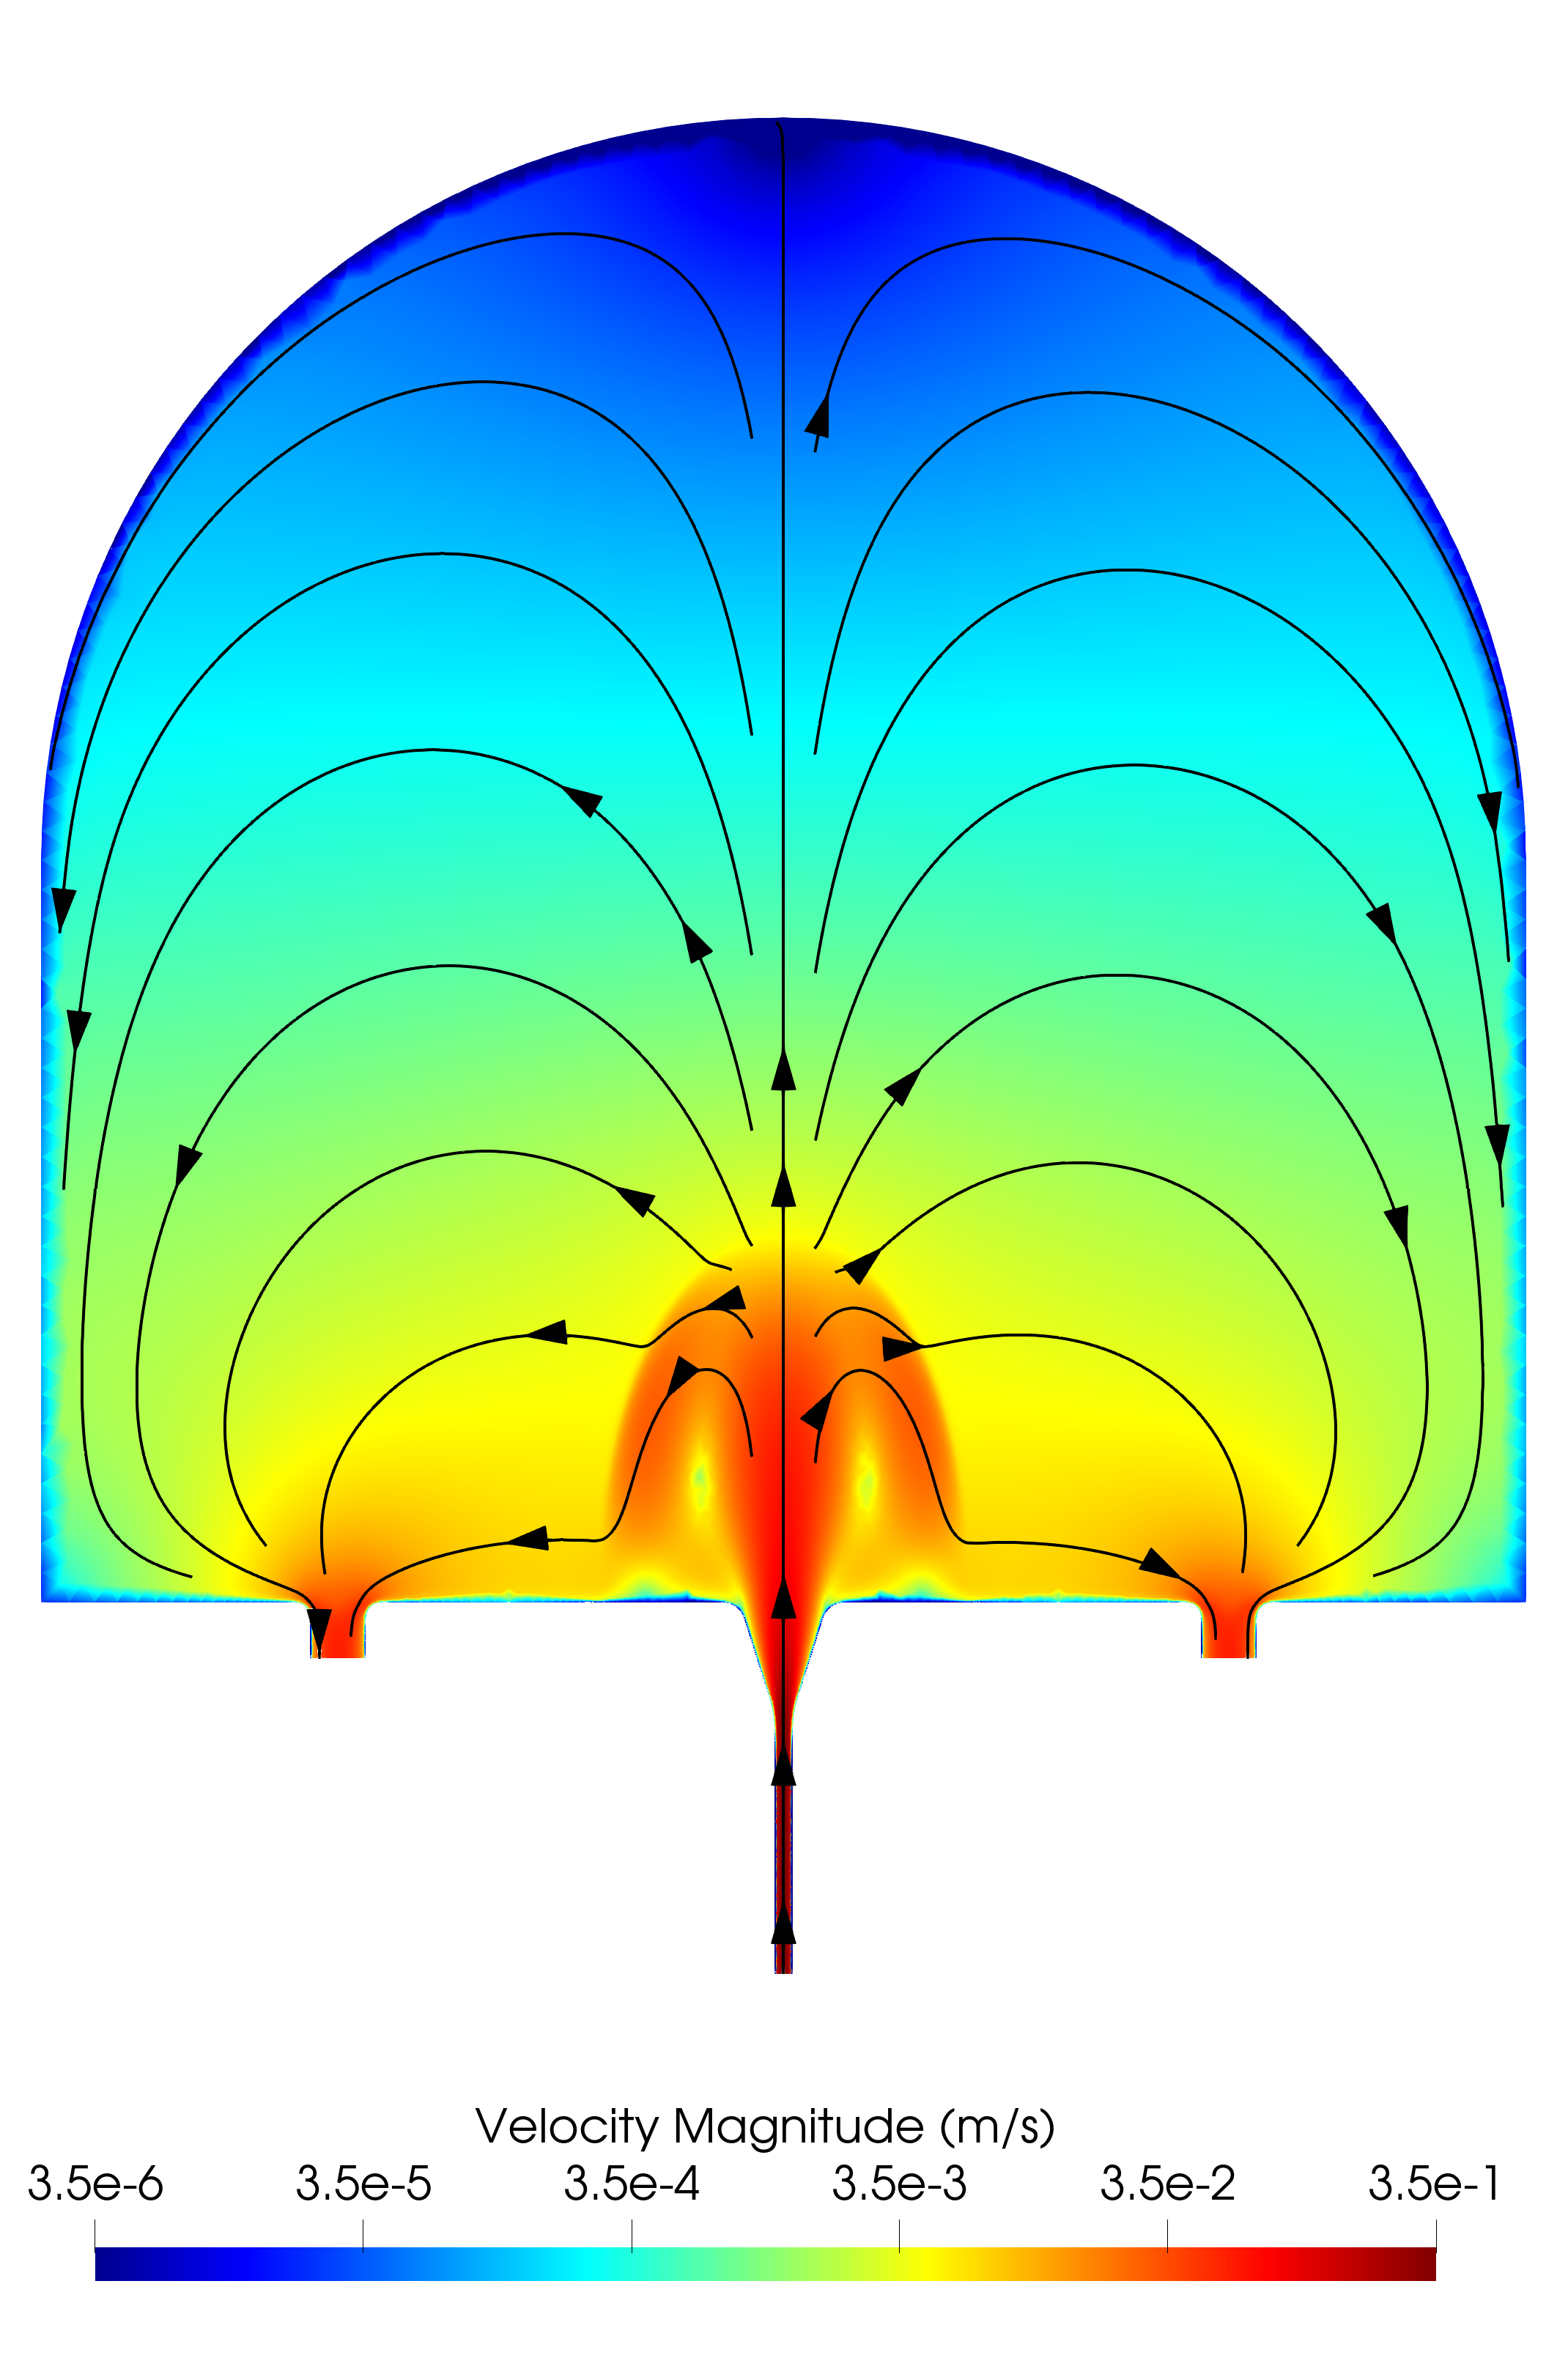
\includegraphics[width=\textwidth]{diagrams/results-modelling/velocity-transport/meshandsoln_dg_velocity_placentone_ns-nsb_velocity-log.png}
                    \caption{}
                    \label{fig:4-models-placentone:ns-nsb}
                \end{subfigure}
                \caption{Velocity plot on placentone geometry (\S\ref{sec:modelling:geometries:2d-placentone}) presenting the results of \S\ref{sec:numerical-methods:blood-flow-experiments:comparison} for the three velocity models: \textbf{NSD} from equation \eqref{eq:nsb}, \textbf{S-B} from equation \eqref{eq:s-b}, and \textbf{NS-NSD} from equation \eqref{eq:ns-nsb}. Plots show a logarithmically-scaled velocity colouring and streamlines shown in black for (a) NSD, (b) S-B, and (c) NS-NSD. All models apply boundary conditions and problem parameters presented in \S\ref{sec:modelling:blood-flow:boundary-conditions}.}
                \label{fig:4-models-placentone}
            \end{figure}
    
            \begin{figure}
                % GENERATED WITH MONOLITH COMMIT: XXX
                % GENERATED ON 2024-XX-XX
                \centering
                \begin{subfigure}[b]{\textwidth}
                    \centering
                    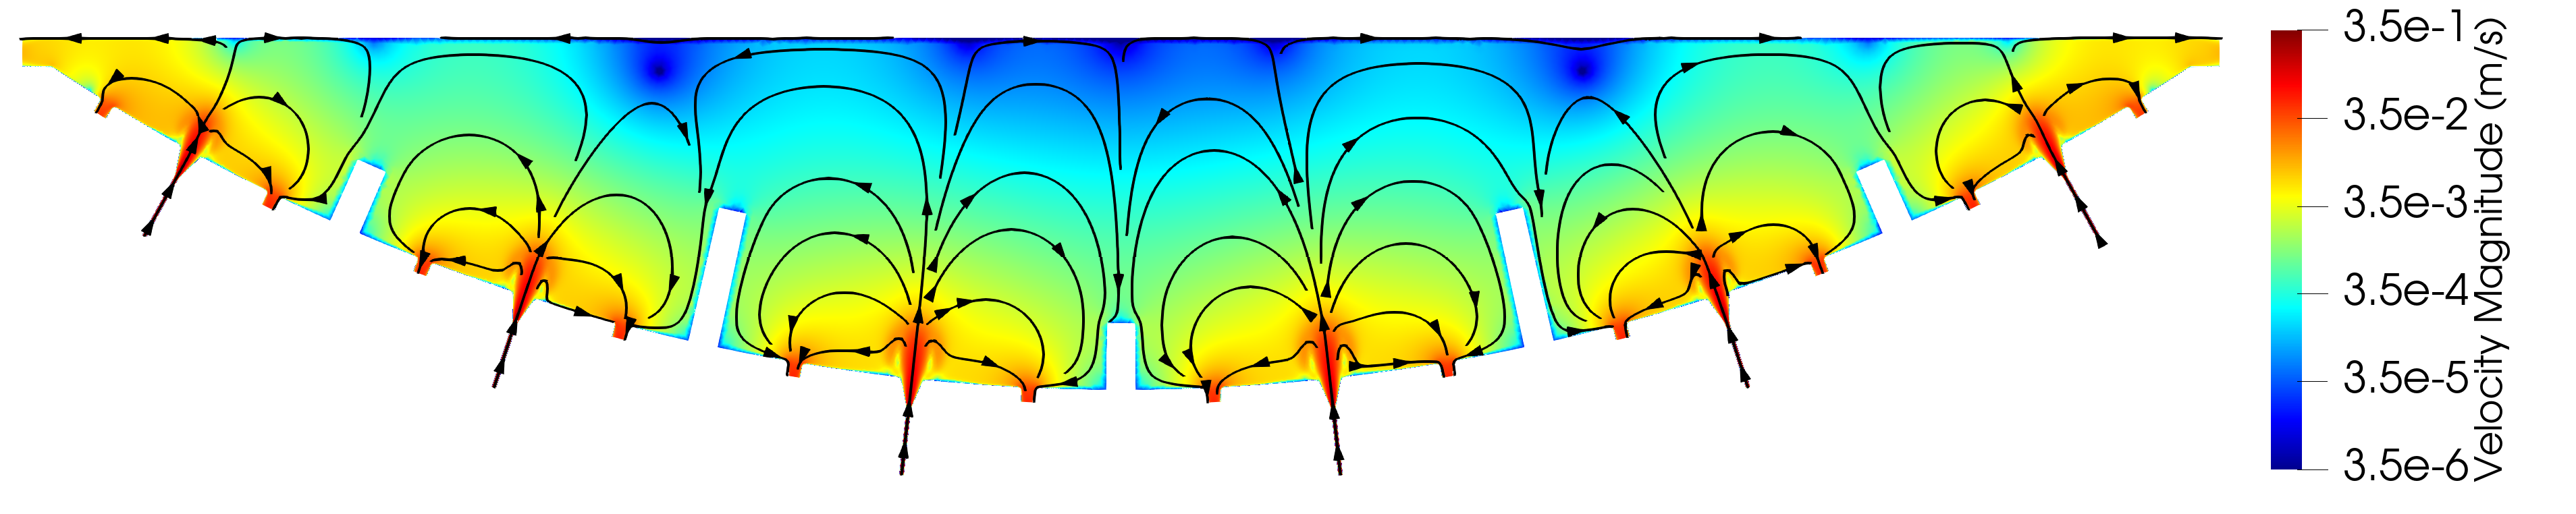
\includegraphics[width=\textwidth]{diagrams/results-modelling/velocity-transport/meshandsoln_dg_velocity_placenta_nsb_velocity-log.png}
                    \caption{}
                    \label{fig:4-models-placenta:nsb}
                \begin{subfigure}[b]{\textwidth}
                    \centering
                    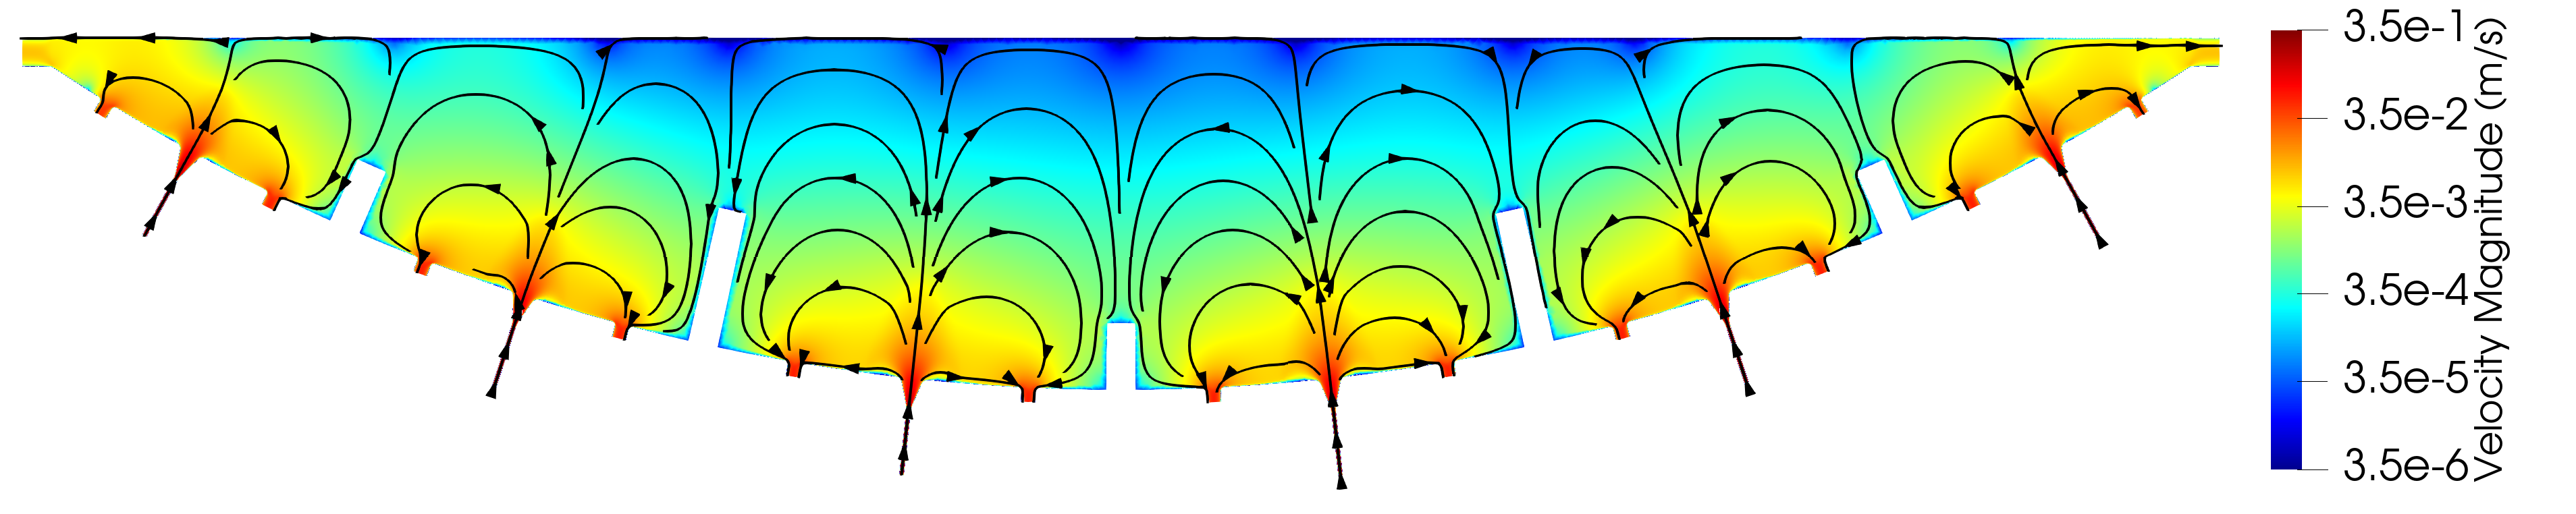
\includegraphics[width=\textwidth]{diagrams/results-modelling/velocity-transport/meshandsoln_dg_velocity_placenta_s-b_velocity-log.png}
                    \caption{}
                    \label{fig:4-models-placenta:s-b}
                \end{subfigure}
                \hfill
                \begin{subfigure}[b]{\textwidth}
                    \centering
                    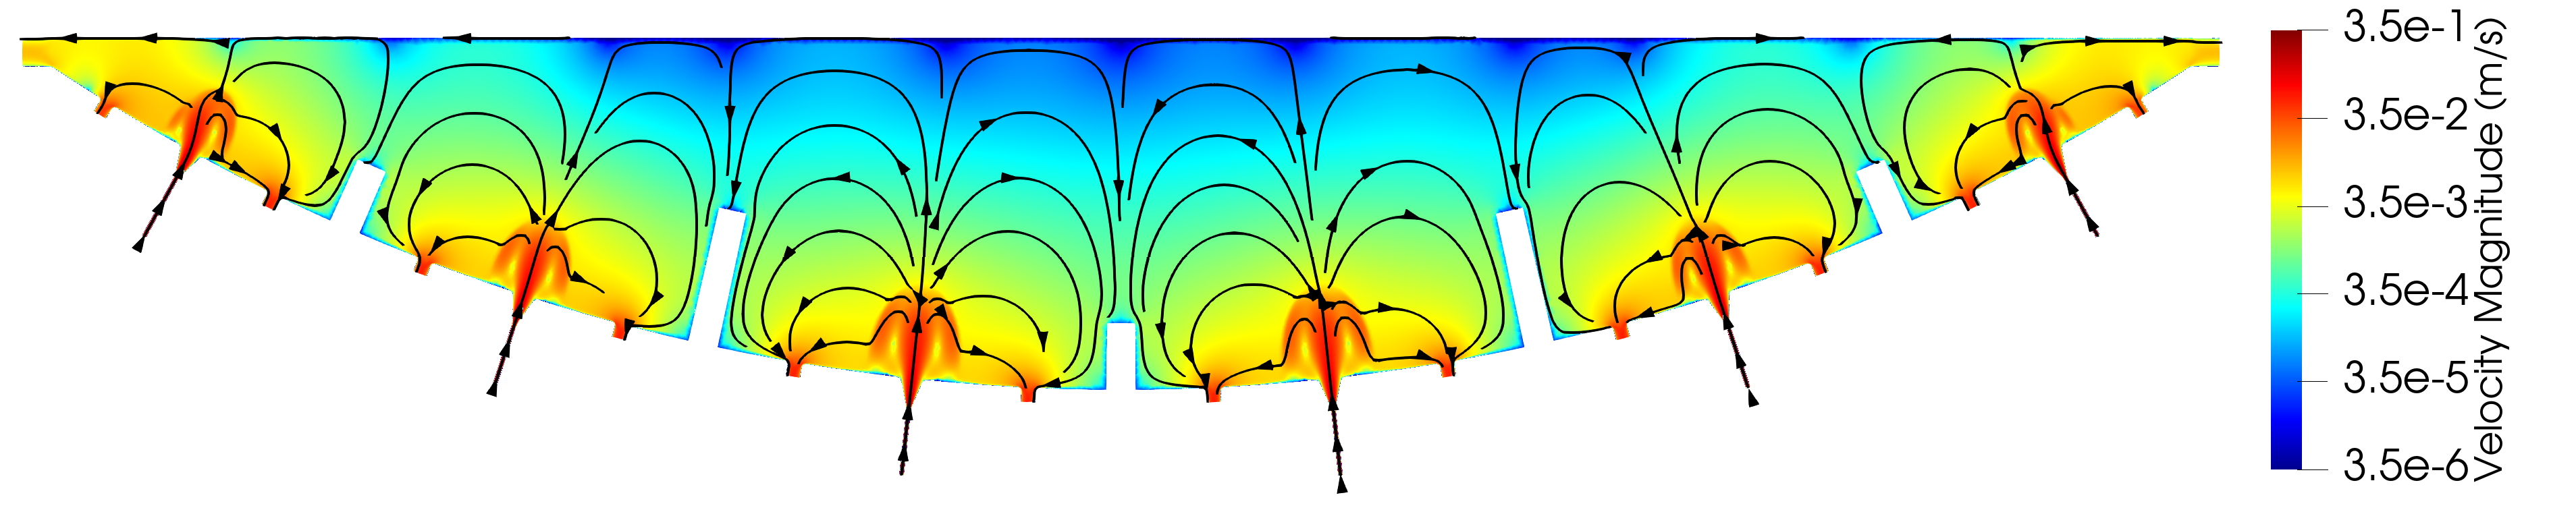
\includegraphics[width=\textwidth]{diagrams/results-modelling/velocity-transport/meshandsoln_dg_velocity_placenta_ns-nsb_velocity-log.png}
                    \caption{}
                    \label{fig:4-models-placenta:ns-nsb}
                \end{subfigure}
                \end{subfigure}
                \caption{Velocity plot on placenta geometry (\S\ref{sec:modelling:geometries:2d-placenta}) presenting the results of \S\ref{sec:numerical-methods:blood-flow-experiments:comparison} for the three velocity models: \textbf{NSD} from equation \eqref{eq:nsb}, \textbf{S-B} from equation \eqref{eq:s-b}, and \textbf{NS-NSD} from equation \eqref{eq:ns-nsb}. Plots show a logarithmically-scaled velocity colouring and streamlines shown in black for (a) NSD, (b) S-B, and (c) NS-NSD. All models apply boundary conditions and problem parameters presented in \S\ref{sec:modelling:blood-flow:boundary-conditions}.}
                \label{fig:4-models-placenta}
            \end{figure}
    
            \begin{figure}
                % GENERATED WITH MONOLITH COMMIT: XXX
                % GENERATED ON 2024-XX-XX
                % \centering
                % \begin{subfigure}[b]{0.45\textwidth}
                    \centering
                    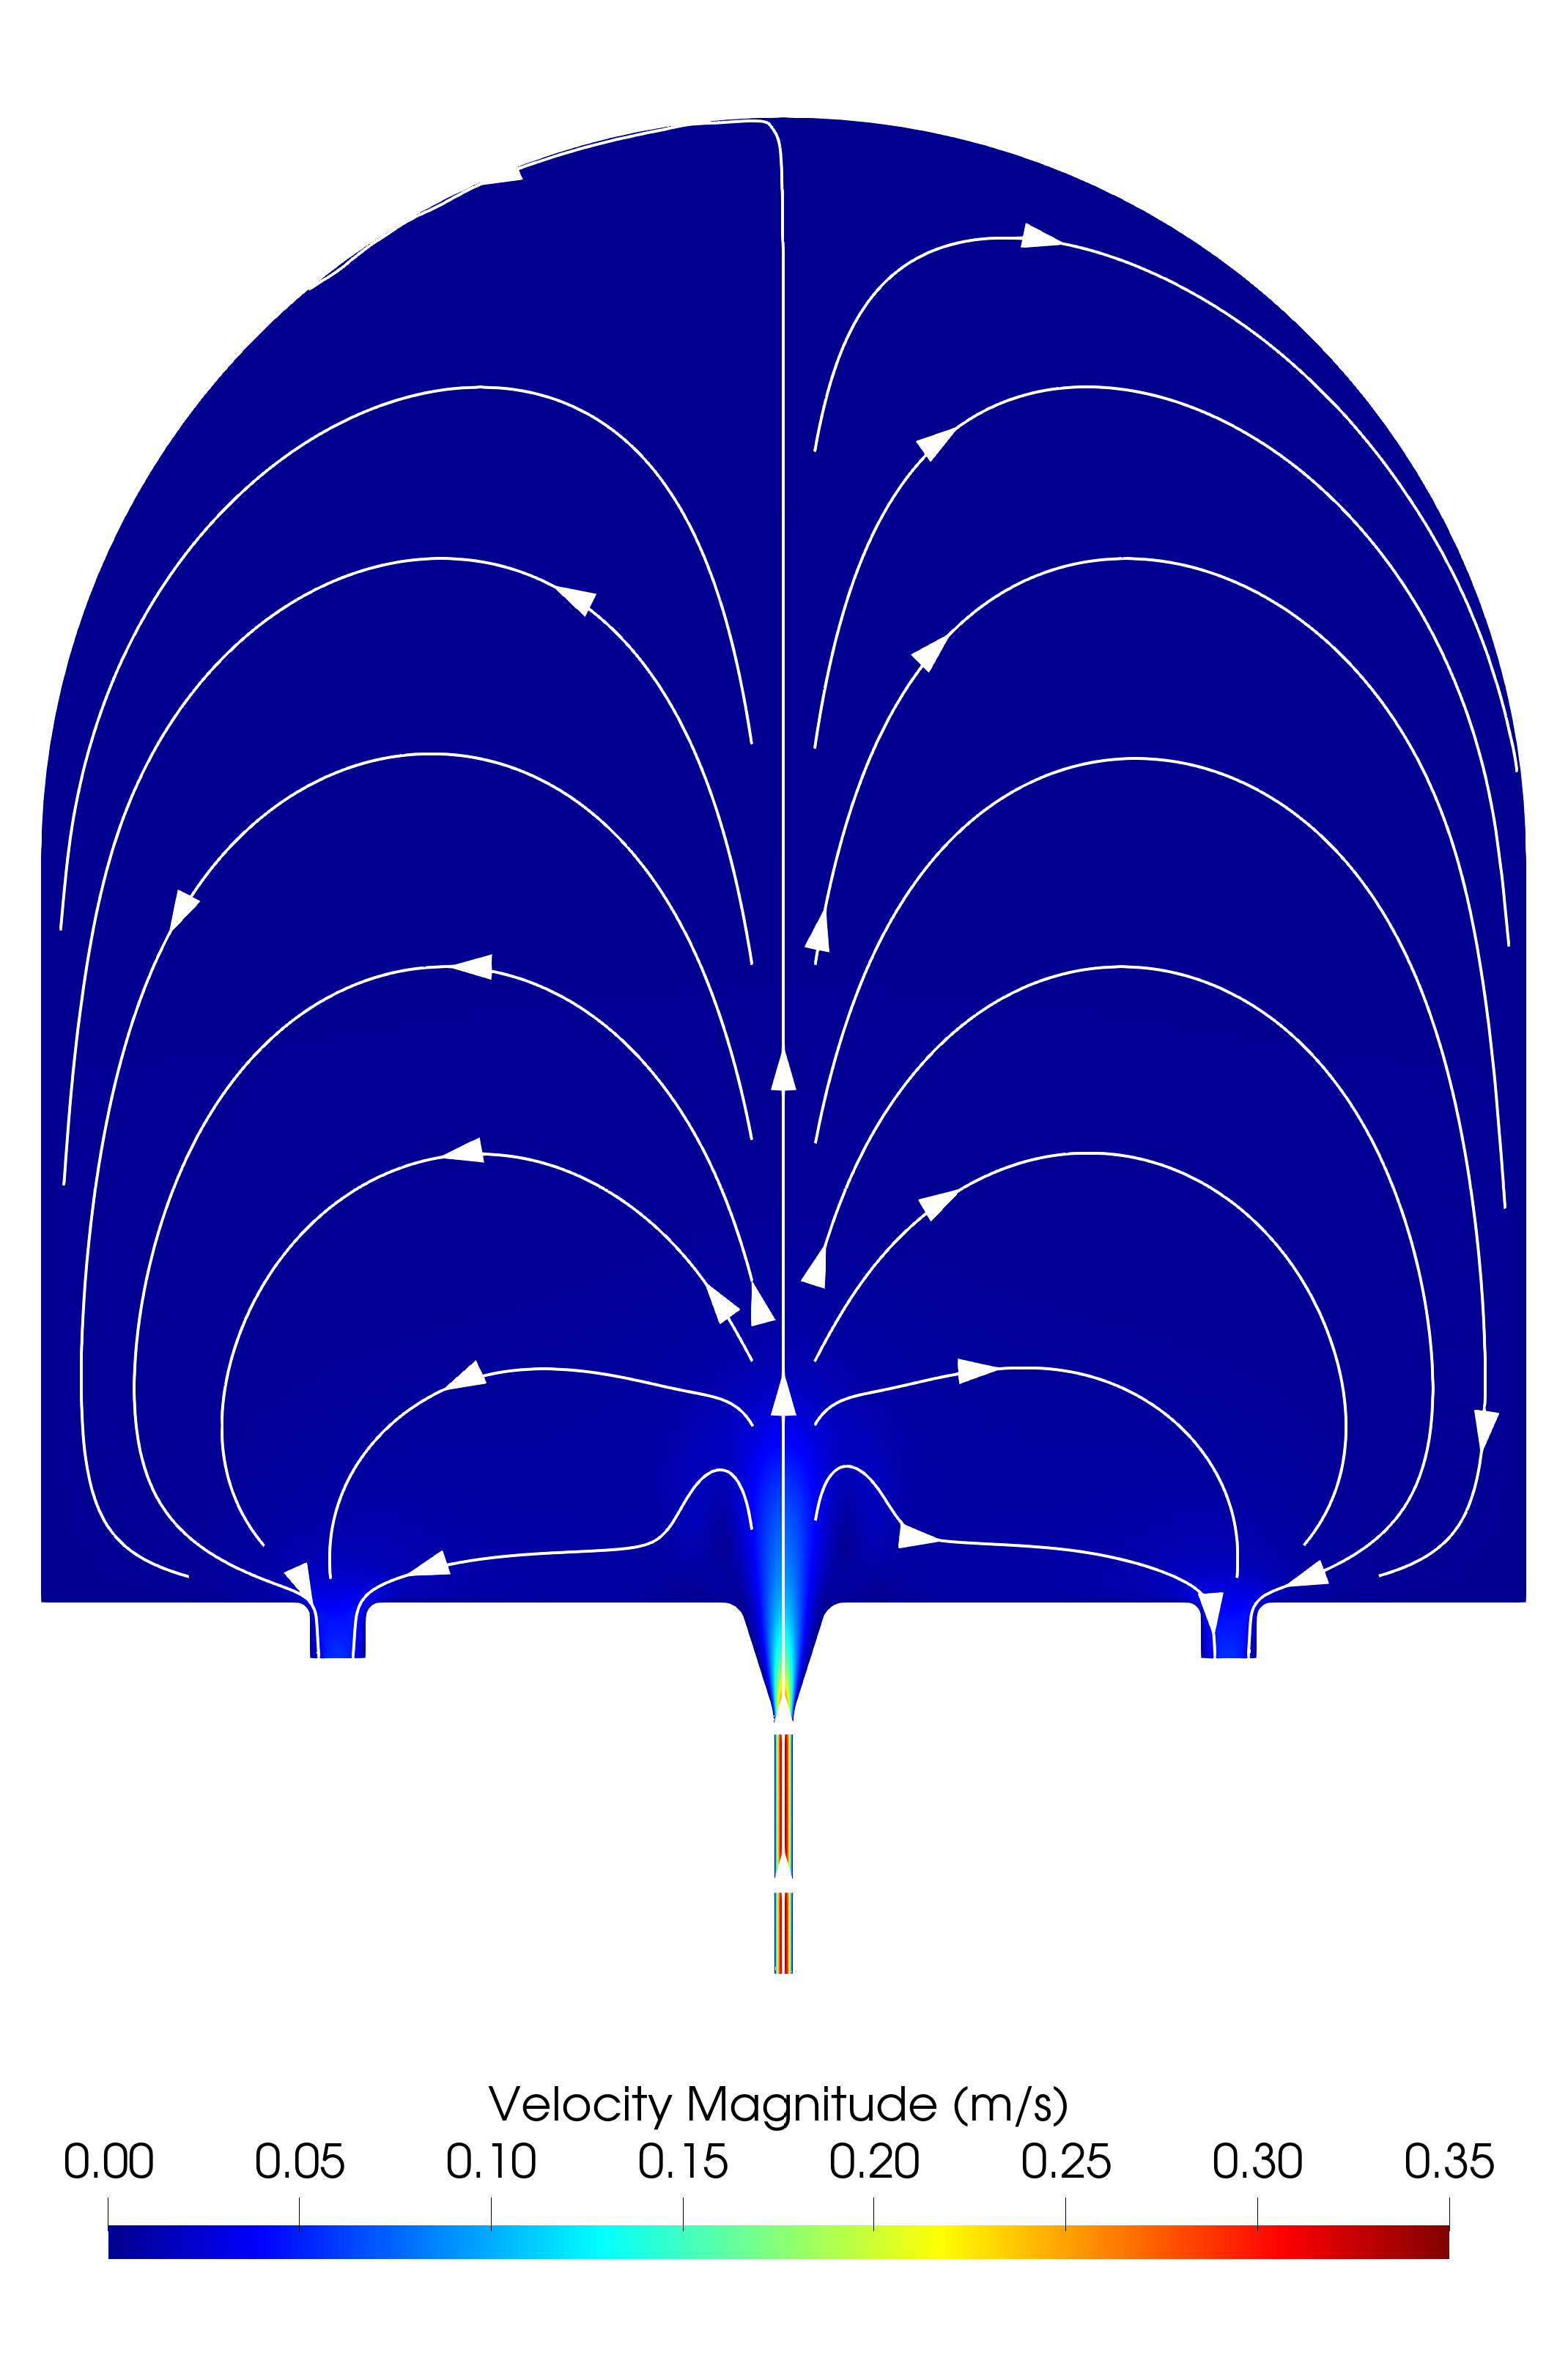
\includegraphics[width=0.5\textwidth]{diagrams/results-modelling/velocity-transport/meshandsoln_dg_velocity_placentone_nsb_velocity-linear.png}
                    \caption{Velocity plot for NSD from Equation \eqref{eq:nsb} on placentone geometry, with \textit{linearly}-scaled velocity colouring and streamlines shown in white. Boundary conditions and problem parameters presented in \S\ref{sec:modelling:blood-flow:boundary-conditions}.}
                    \label{fig:4-models-placentone-linear:nsb}
                % \end{subfigure}
                % \hfill
                % \begin{subfigure}[b]{0.45\textwidth}
                %     \centering
                %     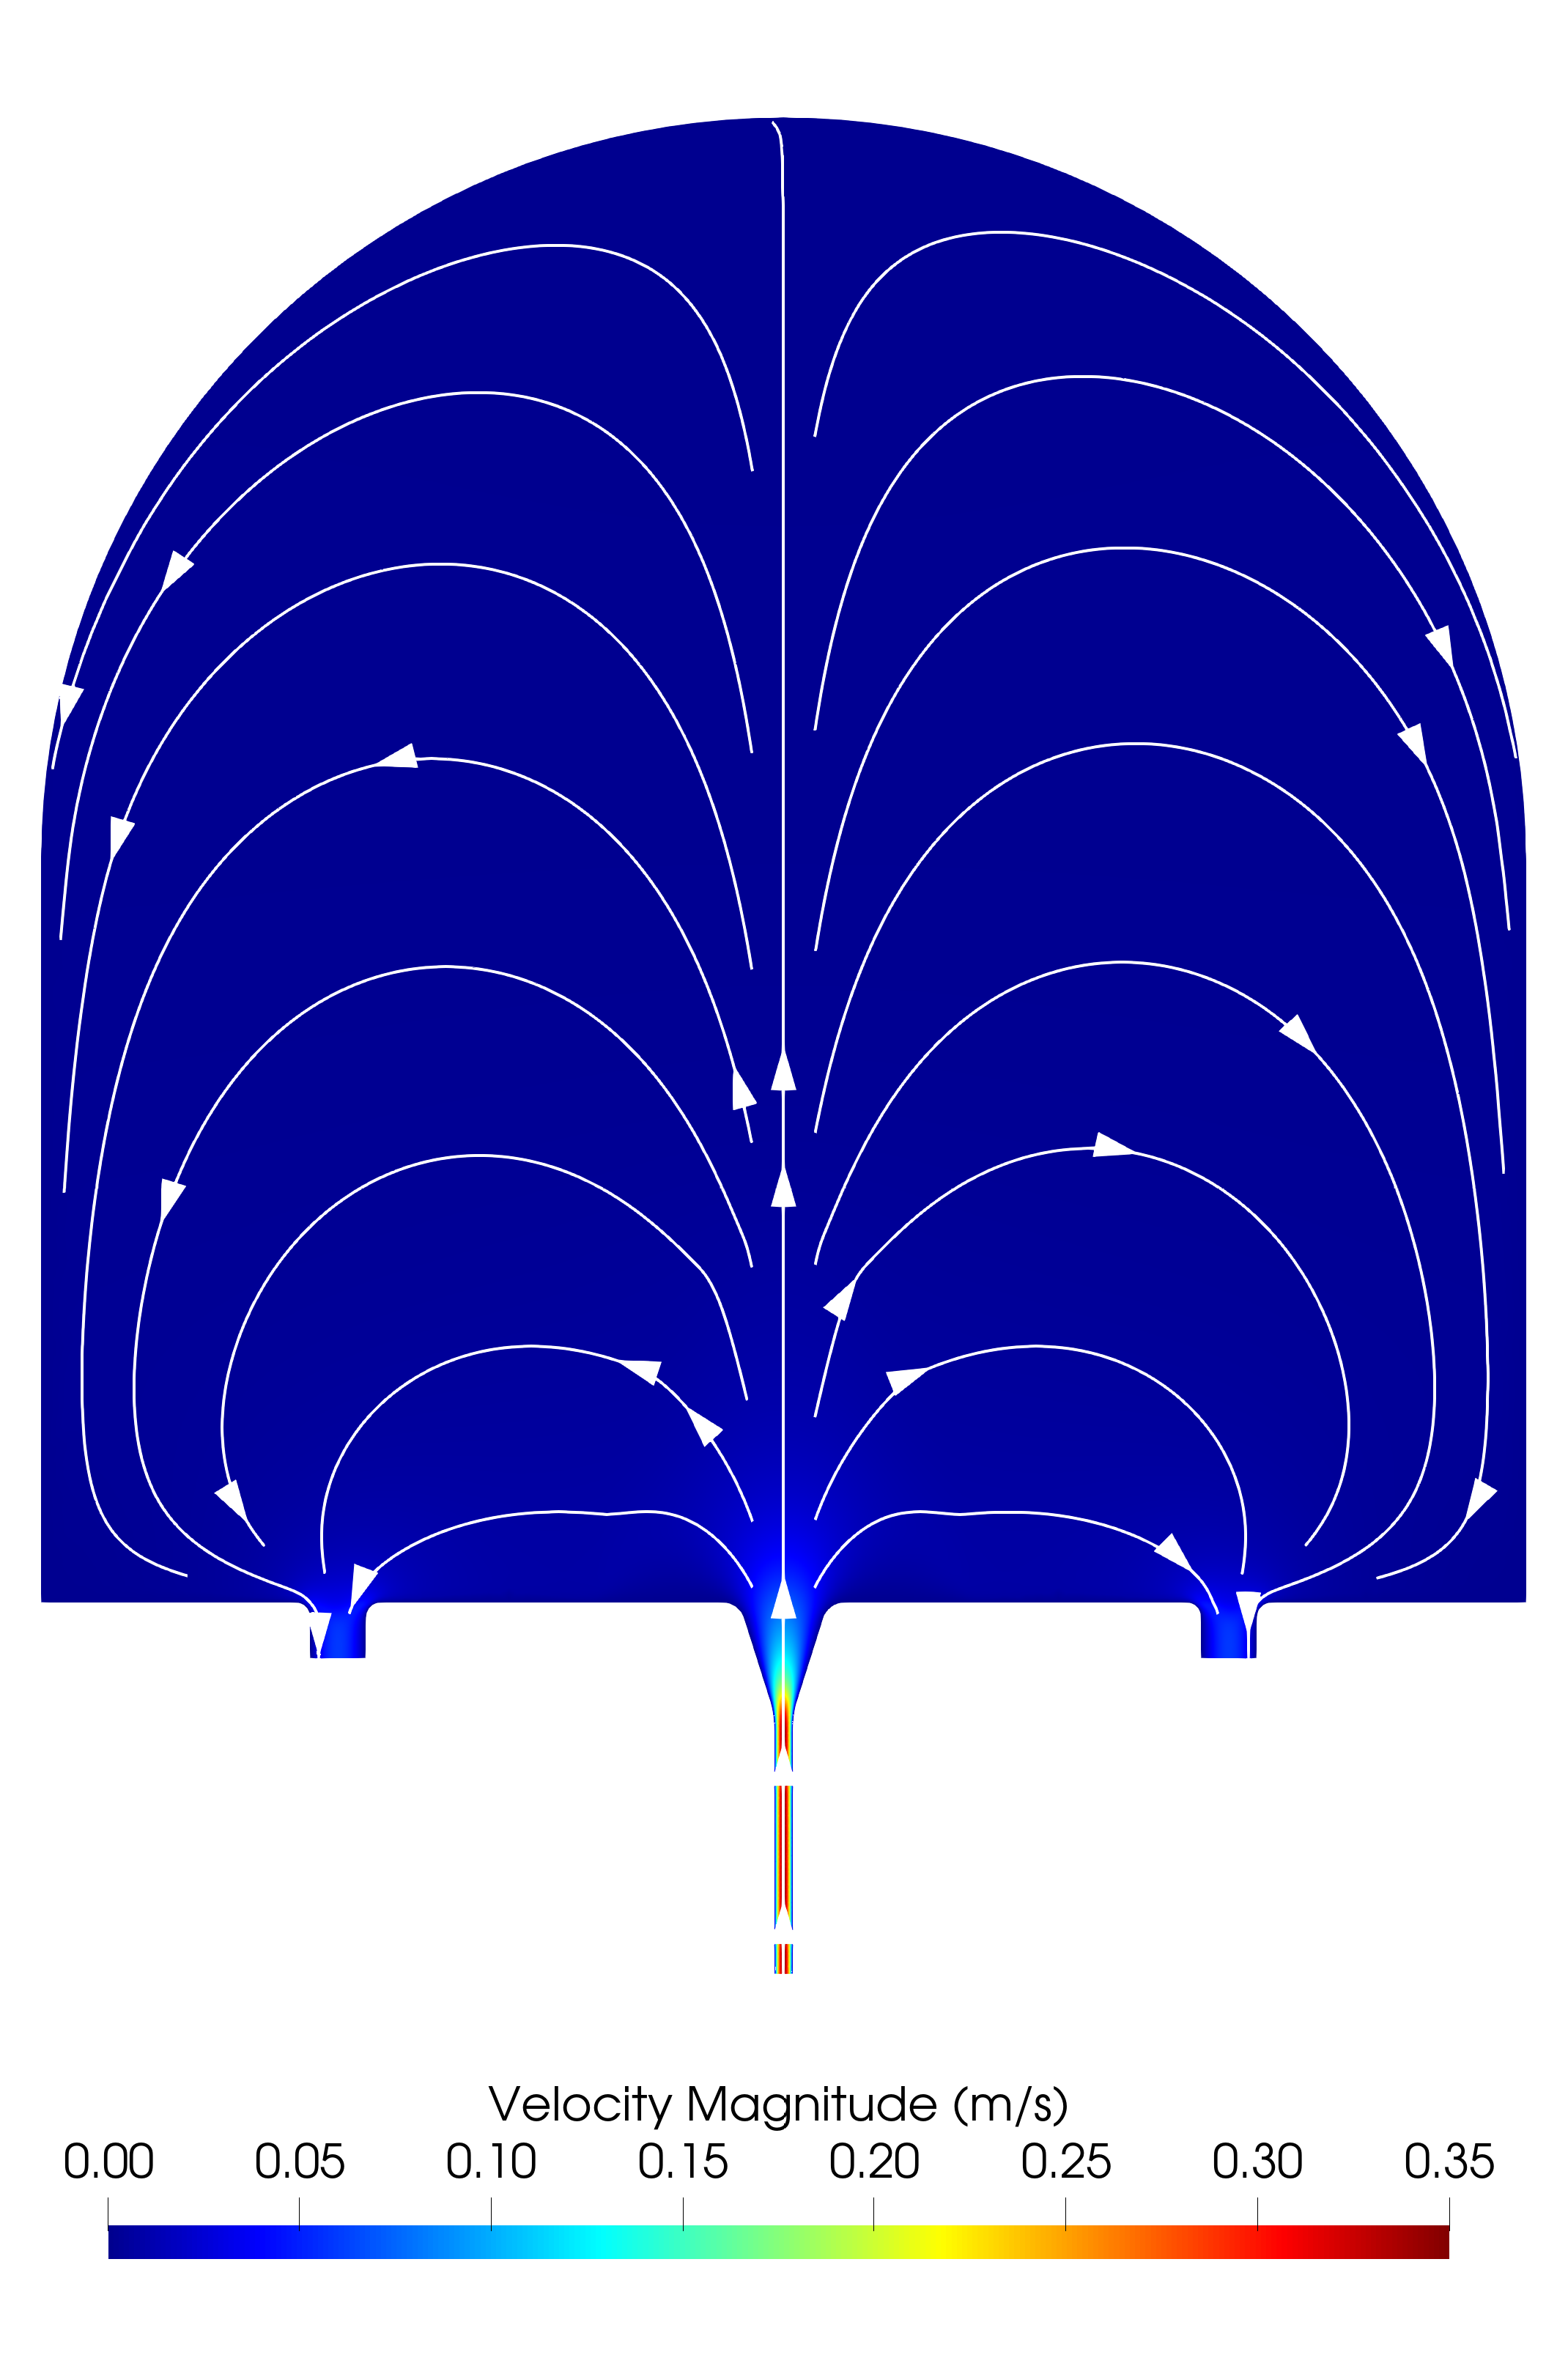
\includegraphics[width=\textwidth]{diagrams/results-modelling/velocity-transport/meshandsoln_dg_velocity_placentone_s-b_velocity-linear.png}
                %     \caption{}
                %     \label{fig:4-models-placentone-linear:s-b}
                % \end{subfigure}
                % \caption{Velocity plot on placentone geometry, with linearly-scaled velocity colouring and streamlines shown in white for (a) NSD, and (b) S-B.}
                % \label{fig:4-models-placentone-linear}
            \end{figure}
            
            Focussing firstly on the simulation using NSD on a placentone presented in Figure \ref{fig:4-models-placentone:nsb}, the flow is symmetric about the artery, forming two small recirculation zones in the central cavity (CC). The flow then decelerates as it passes from the CC to the IVS, with some of the flow decelerating even further as it passes higher up into the IVS. The flow then accelerates again when exiting through one of the two basal plate veins. It is worth mentioning that the colours corresponding to the velocity magnitude here are given on a logarithmic scale, rather than a linear scale. This is because the flows presented here decelerate very quickly after leaving the artery, due to the low permeability of the IVS (see Table \ref{tab:problem-parameters} and \S\ref{sec:modelling:blood-flow}). By plotting on a logarithmic scale, we can more clearly see the behaviour of the fluid in all regions of the domain. To demonstrate this, the same simulation from Figure \ref{fig:4-models-placentone:nsb} is plotted again on a linear scale in Figure \ref{fig:4-models-placentone-linear:nsb}, where almost all the flow appears close to zero outside of the artery. We notice that by visualising on a logarithmic scale, we can see some discontinuities near the boundaries, visible on the edges of the underlying mesh triangulation; these discontinuities are relatively small at $\mathcal{O}(\num{1e-5})\unit{\metre\per\second}$ and are due to the weak imposition of boundary conditions by the numerical method (see \S\ref{sec:numerical-methods:equation-discretisations:nsd} for further details).
    
            Turning our attention to the other two simulations presented in Figure \ref{fig:4-models-placentone}, we see that all three models demonstrate largely the same behaviour, whereby high-speed flow is concentrated in the central-cavity, artery, and veins. However, one notable difference between the S-B simulation in Figure \ref{fig:4-models-placentone:s-b} and the others is that there are no recirculations in the CC. Another notable difference is visible in Figure \ref{fig:4-models-placentone:ns-nsb}, showing a simulation NS-NSD, where the blood velocity decelerates quickly when crossing the CC-IVS interface, which is unlike the simulations for NSD and S-B, respectively shown in Figures \ref{fig:4-models-placenta:nsb} and \ref{fig:4-models-placenta:s-b}. The difference with NSD is due to the chosen transition width, $\tau$, from Table \ref{tab:structural-parameters} for the smooth transition function in NSD, which allows flow to decelerate more smoothly between porous and free flow. The reason for differences with S-B is due to the fluid inside the CC decelerating much more gradually in the case of S-B. A related observation is that the recirculation zones for NS-NSD appear further from the basal plate than for NSD, which again is due to the chosen smooth transition width for NSD. Appendix \ref{sec:flow-comparison} further investigates the differences in flow between the three models on a placentone.
            
            Figure \ref{fig:4-models-placenta} presents the simulations for the three velocity models on a placenta geometry. The overall behaviour is similar to that described above in the placentone geometry, except flow may now exit through one of the newly introduced marginal sinus veins, or through basal plate veins located in other placentones. There are only a small number of streamlines that cross septal walls in these numerical experiments, which is due to the symmetry of the placement of vessels in this particular problem. In the next subsection, \S\ref{sec:numerical-methods:blood-flow-experiments:asymmetric} will present a flow on a geometry with asymmetrically-placed veins to see what impact this has on the flow field.

            This section has shown that IVS flow is very similar for all three velocity models, with differences between some of the models in the central cavity region; in particular, the S-B model failed to capture some of the high-speed flow features present in the cavity of the other two models due to the relatively high Reynolds number at the artery mouth ($\Rey \approx 60$). We select NSD as our blood flow model for the remainder of this thesis as (i) it is advantageous for the DGFEMs we employ (due to not requiring interface conditions at the porous interface), (ii) gives a physiologically sensible transition region between `free' and porous flow, and (iii) avoids non-physical boundary layers that may occur when coupling two fluid PDEs \cite{nealePracticalSignificanceBrinkman1974}. It is worth noting that this model also adds flexibility for future model development beyond this thesis, where regions apart from the central cavity and vessels could be specified with a lower resistance to flow due to the absence of fetal tree material.
    
        \subsection{Asymmetric flow} \label{sec:numerical-methods:blood-flow-experiments:asymmetric}
            We now compute the solution on the placenta geometry where we have included all basal plate arteries in the centre of each placentone, but have included only one basal plate vein per placentone to encourage an asymmetric flow pattern in the placenta (as such asymmetries would be typical in a physical placenta). We place basal plate veins in the widest placentones with \qty{8}{\milli\metre} between their centres and the side walls, and place veins in other placentones proportionally according to the width of each placentone. Note that the larger marginal sinus veins are included here, but not any septal wall veins. We again select model parameters from Tables \ref{tab:structural-parameters} and \ref{tab:problem-parameters} and use the discretisations from \S\ref{sec:numerical-methods:equation-discretisations} to approximate solutions to the steady-state NSD model. The flow field is shown in Figure \ref{fig:asymmetric-placenta}, where the velocity magnitude is shown on a logarithmic colour scale, and streamlines are shown in black.

            \begin{figure}
                %  Resulting from running ./drivers/mri_run.py
                %  Plotted in a separate plotter script ./plotting/placenta-plots.pvsm
                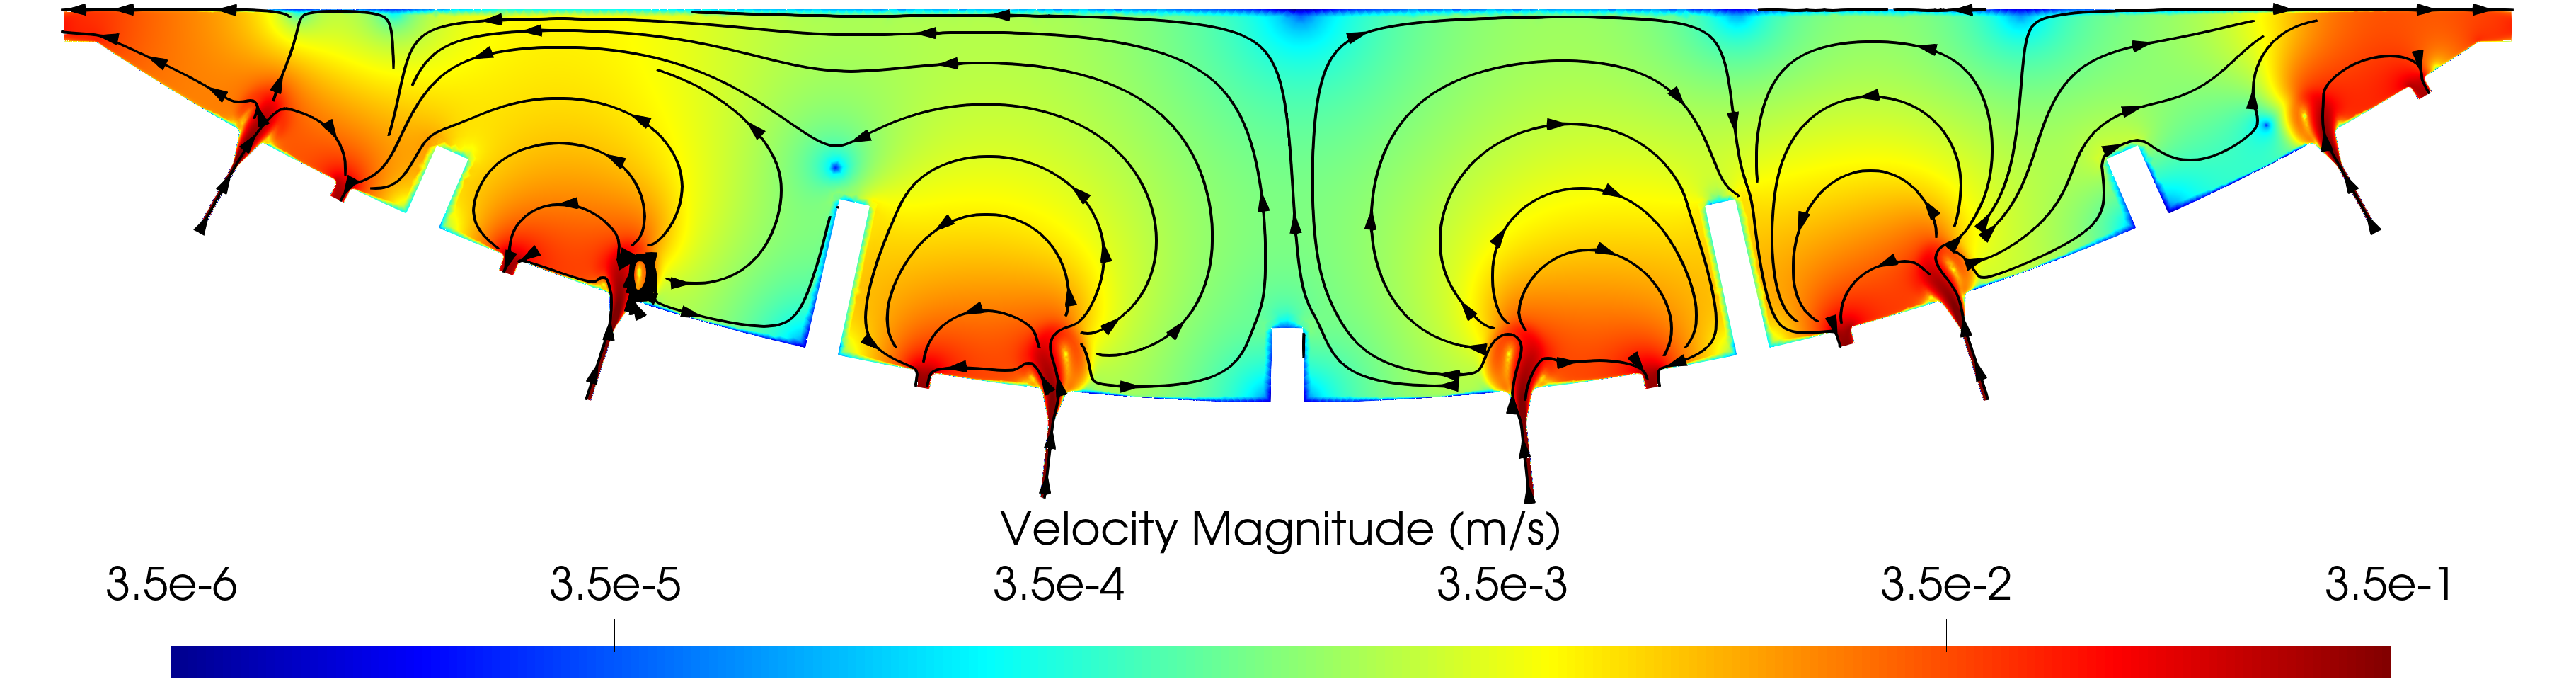
\includegraphics[width=0.9\textwidth]{diagrams/results-mri/simulated-placenta/simulated-placenta-velocity.png}
                \caption{Velocity plot of NSD from Equation \eqref{eq:nsb} on the placenta geometry, with only one basal plate vein per placentone, as described in \S\ref{sec:numerical-methods:blood-flow-experiments:asymmetric}. Shows logarithmically-scaled velocity colouring and streamlines shown in black.}
                \label{fig:asymmetric-placenta}
            \end{figure}

            In this simulation, we see much faster flow in many areas of the domain than that of the simulation where veins have been placed symmetrically about the artery (shown in Figure \ref{fig:4-models-placenta:nsb}). Most notably, we see a much higher proportion of blood flowing over the septal walls. Related to this, there is roughly an order of magnitude faster flow near the chorionic plate (i.e., the top of the domain) as blood traverses the placenta in order to exit either through another placentone's basal plate vein or through one of the two marginal sinus veins.
            
            Despite this faster flow over the septal walls, we recall that the speed of flow is logarithmically coloured here, meaning that the flow over the walls is more than two orders of magnitude slower than the inlet speed. Although cross-placentone flow may be an important mechanism of placenta functionality, the faster regions of flow remain concentrated near the spiral artery mouth. Interestingly, this fast flow region is larger than the region shown in the symmetric simulation (Figure \ref{fig:4-models-placenta:nsb}), stretching in a dome-like shape over the area between each basal plate artery and vein pair. This is giving the blood an opportunity to `short-circuit', where flow almost immediately exits the placenta, potentially advecting high concentrations of oxygen with it.

            The simulation presented in this section demonstrates an order of magnitude faster flow near the chorionic plate when veins are placed asymmetrically. Whilst several mathematical studies have assumed symmetric placement of veins, this is physiologically unlikely, with large variations in numbers of veins and their placement between different placentas (see discussion in Chapter \ref{sec:introduction}). The simulation presented here will be used as the basis of investigations in Chapters \ref{sec:numerical-mri} and \ref{sec:contractions}, where we will respectively investigate MRI signals and placental contractions. The next section presents the corresponding oxygen concentration field to this asymmetric velocity field.

    \section{Oxygen transport numerical experiments} \label{sec:numerical-methods:nutrient-transport-experiments}
        Here, we present a basic numerical experiment to demonstrate the behaviour of the steady-state oxygen transport model, advected by blood flow according to the NSD flow model in Equation \eqref{eq:nsb}. Figure \ref{fig:transport-placenta} shows oxygen concentration on the placenta geometry, where the basal plate veins have been placed asymmetrically as presented in \S\ref{sec:numerical-methods:blood-flow-experiments:asymmetric}, and model parameters are selected from Table \ref{tab:problem-parameters} according to common choices in the literature.

        \begin{figure}
            \centering
            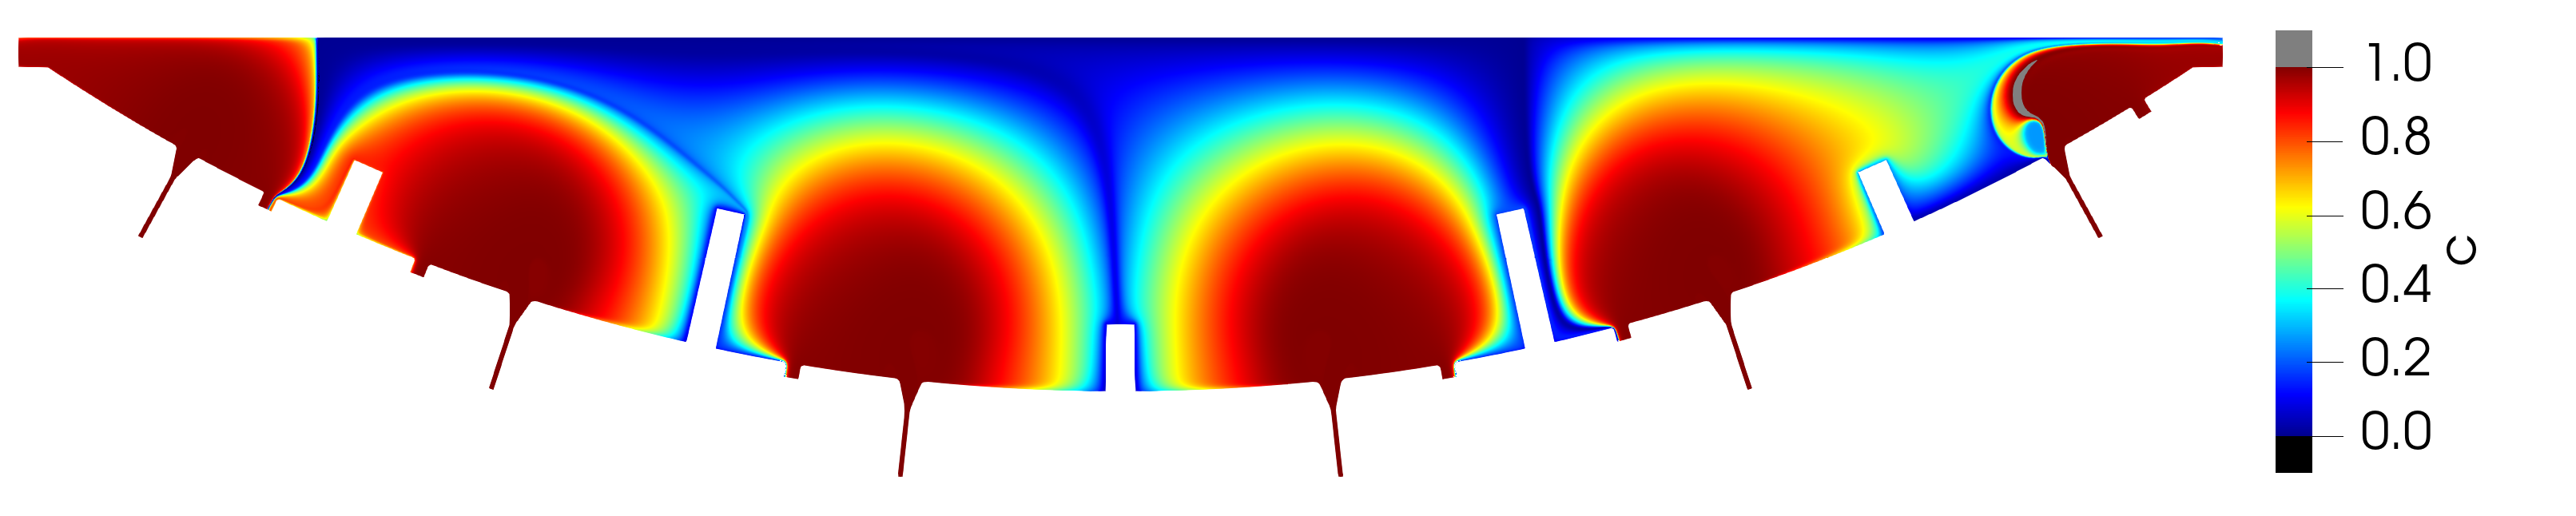
\includegraphics[width=\textwidth]{diagrams/results-modelling/velocity-transport/oxygen_asymmetric.png}
            \caption{Oxygen concentration plot for the reaction-advection-diffusion equation from Equation \eqref{eq:rad}, with one vein per placentone as described in \S\ref{sec:numerical-methods:nutrient-transport-experiments}. The colour scale varies between $0$ (no concentration) and $1$ (maximum concentration). Under- and over-shoots in the approximate solution are respectively coloured in black and grey.}
            \label{fig:transport-placenta}
        \end{figure}

        We see that the oxygen penetrates the IVS radially from each artery in high concentration ($c \approx $ 1), following the streamlines of the underlying flow from Figure \ref{fig:asymmetric-placenta} through the IVS, and ultimately exiting through any one of the basal plate or marginal sinus veins. The oxygen concentration above most placentones lowers to $c \approx 0$ towards the chorionic plate, with the gradient at which concentration lowers toward the chorionic plate differing greatly from placentone-to-placentone. In the left-most placentone, very high concentrations of oxygen reach the chorionic plate, which is then transported out a marginal sinus vein, also in high concentration. In fact, most of the exiting blood through all of the veins contains a high oxygen concentration. This is physiologically surprising, as this is oxygen that could have been uptaken by the villous tree given the right conditions, but instead exits the placenta and returns to the maternal circulation. We will investigate oxygen uptake further in Chapter \ref{sec:nutrient-uptake}.

        The oxygen concentration is notably low above the central septal wall, likely due to the symmetry in the vessel placement in the two centre-most placentones. Differing from previous studies that consider oxygen transport on placentones, the flow in this placenta geometry can transport oxygen over the septal walls, and does so most notably above the outer-most septal walls. In these cases, oxygen is advected to neighbouring placentones, ultimately exiting through a basal plate vein or marginal sinus vein. Interestingly, the oxygen in these cases decreases far more than those that exit through closer veins; this is due to the longer transit time of the oxygen, which allows more oxygen to be uptaken by the villous tree, as the blood is drawn over longer distances at relatively slow speed before exiting. We also see in these cases a very small region of low oxygen concentration trapped between two regions of higher concentration; this is due to the streamlines of the underlying flow, which do not cross, and have here advected oxygen of low concentration from near the chorionic or basal plates. 

        An advantage of using DGFEM in approximating of the blood flow field is the reduction in spurious oscillations, which are typically present in flow fields such as this with continuous finite element methods. However, the discontinuous oxygen concentration field instead results in small, contained numerical artefacts in the oxygen concentration field. In particular, numerical artefacts may be present in areas where there are steep gradients in the oxygen concentration field. For this problem, there is an overshoot above $c = 1$ in the right-most placentone originating from a recirculation zone. A convergence study verified that these artefacts reduce in amplitude under mesh refinement, and have minimal impact on any resulting quantities computed from the oxygen concentration field (i.e., the measures computed later in Chapter \ref{sec:nutrient-uptake}).
        
        Overall, most of the high oxygen concentration is confined to placentones here, which is due to the number and positioning of the arteries and veins. Later in the thesis, Chapter \ref{sec:nutrient-uptake} will investigate how the number and placement of vessels affects the oxygen concentration field in more depth.

    \section{Time-dependent blood flow and oxygen transport experiments} \label{sec:numerical-methods:time-dependent-experiments}
        We have so far presented only steady-state numerical experiments corresponding to flow at peak systole. We will now present some numerical experiments that are time-dependent, and use the time-dependent versions of the discretisations of both the blood flow and oxygen transport models that were presented in \S\ref{sec:numerical-methods:equation-discretisations} on the 2D placenta geometry. We once again select parameters from Tables \ref{tab:structural-parameters} and \ref{tab:problem-parameters} and place veins asymmetrically as presented in \S\ref{sec:numerical-methods:blood-flow-experiments:asymmetric}.
        
        We follow work by \citeauthor{carsonPersonalisingCardiovascularNetwork2021} \cite{carsonPersonalisingCardiovascularNetwork2021} and apply a pulsatile boundary condition on the inlet arteries, where we use the profile given in Figure 4(H) of \cite{carsonPersonalisingCardiovascularNetwork2021} to give the amplitude, which is representative of in vivo pulsatile flow. We used \href{https://apps.automeris.io/wpd/}{WebPlotDigitizer}\footnote{\url{https://apps.automeris.io/wpd/}} to read in the amplitude data $A(t)$ from \cite{carsonPersonalisingCardiovascularNetwork2021}, and shifted and scaled the data such that $t=0$ corresponds to the first peak and $U(0) = \qty{0.35}{\metre\per\second}$; we then assumed periodicity between the first and second peaks to give amplitudes for all $t$. We run the simulation for $t \in [0, T_N]$, where $T_N = 3.34$ and corresponds to five cardiac cycles. $A(t)$ is illustrated in Figure \ref{fig:oscillating-inlet-amplitude}, which corresponds to the amplitude of the Poiseuille flow on all six artery inlets. This involves applying modified boundary conditions to the flow to
        \begin{subequations}
            \begin{alignat}{3}
                \vec{g}_\text{f,D} & = - A(t) \frac{R^2 - r^2}{R^2} \vec{n} &&~ \text{on } \Gamma_\text{in},\label{eq:modified-amplitude-flow-bcs:1}\\
                \vec{g}_\text{f,N} & = \vec{0} &&~ \text{on } \Gamma_\text{out},\label{eq:modified-amplitude-flow-bcs:2}\\
                \vec{g}_\text{f,D} & = \vec{0} &&~ \text{on } \Gamma \setminus (\Gamma_\text{in} \cup \Gamma_\text{out}),\label{eq:modified-amplitude-flow-bcs:3}
            \end{alignat}%
            \label{eq:modified-amplitude-flow-bcs}%
        \end{subequations}%
        where $\vec{n}$ is the unit outward-pointing normal on $\Gamma_\text{in}$, $r(\vec{x})$ is the distance from a point $\vec{x}$ to the centre of $\Gamma_\text{in}$, $R$ is the artery radius, and $A(t)$ is the amplitude of the Poiseuille inlet flow. The procedure we employ is to generate solutions of both the blood flow and oxygen concentration by first solving their steady-state equations, and then feeding this as an initial condition into the time-dependent equations. In this simulation, basal plate veins have been placed asymmetrically as presented in \S\ref{sec:numerical-methods:blood-flow-experiments:asymmetric}, model parameters are selected from Table \ref{tab:problem-parameters}, and we select $\Delta t = \qty{0.03336}{\second}$ (i.e., $100$ time-steps for $t \in [0, 3.336] \, \unit{\second}$).

        \begin{figure}
            \centering
            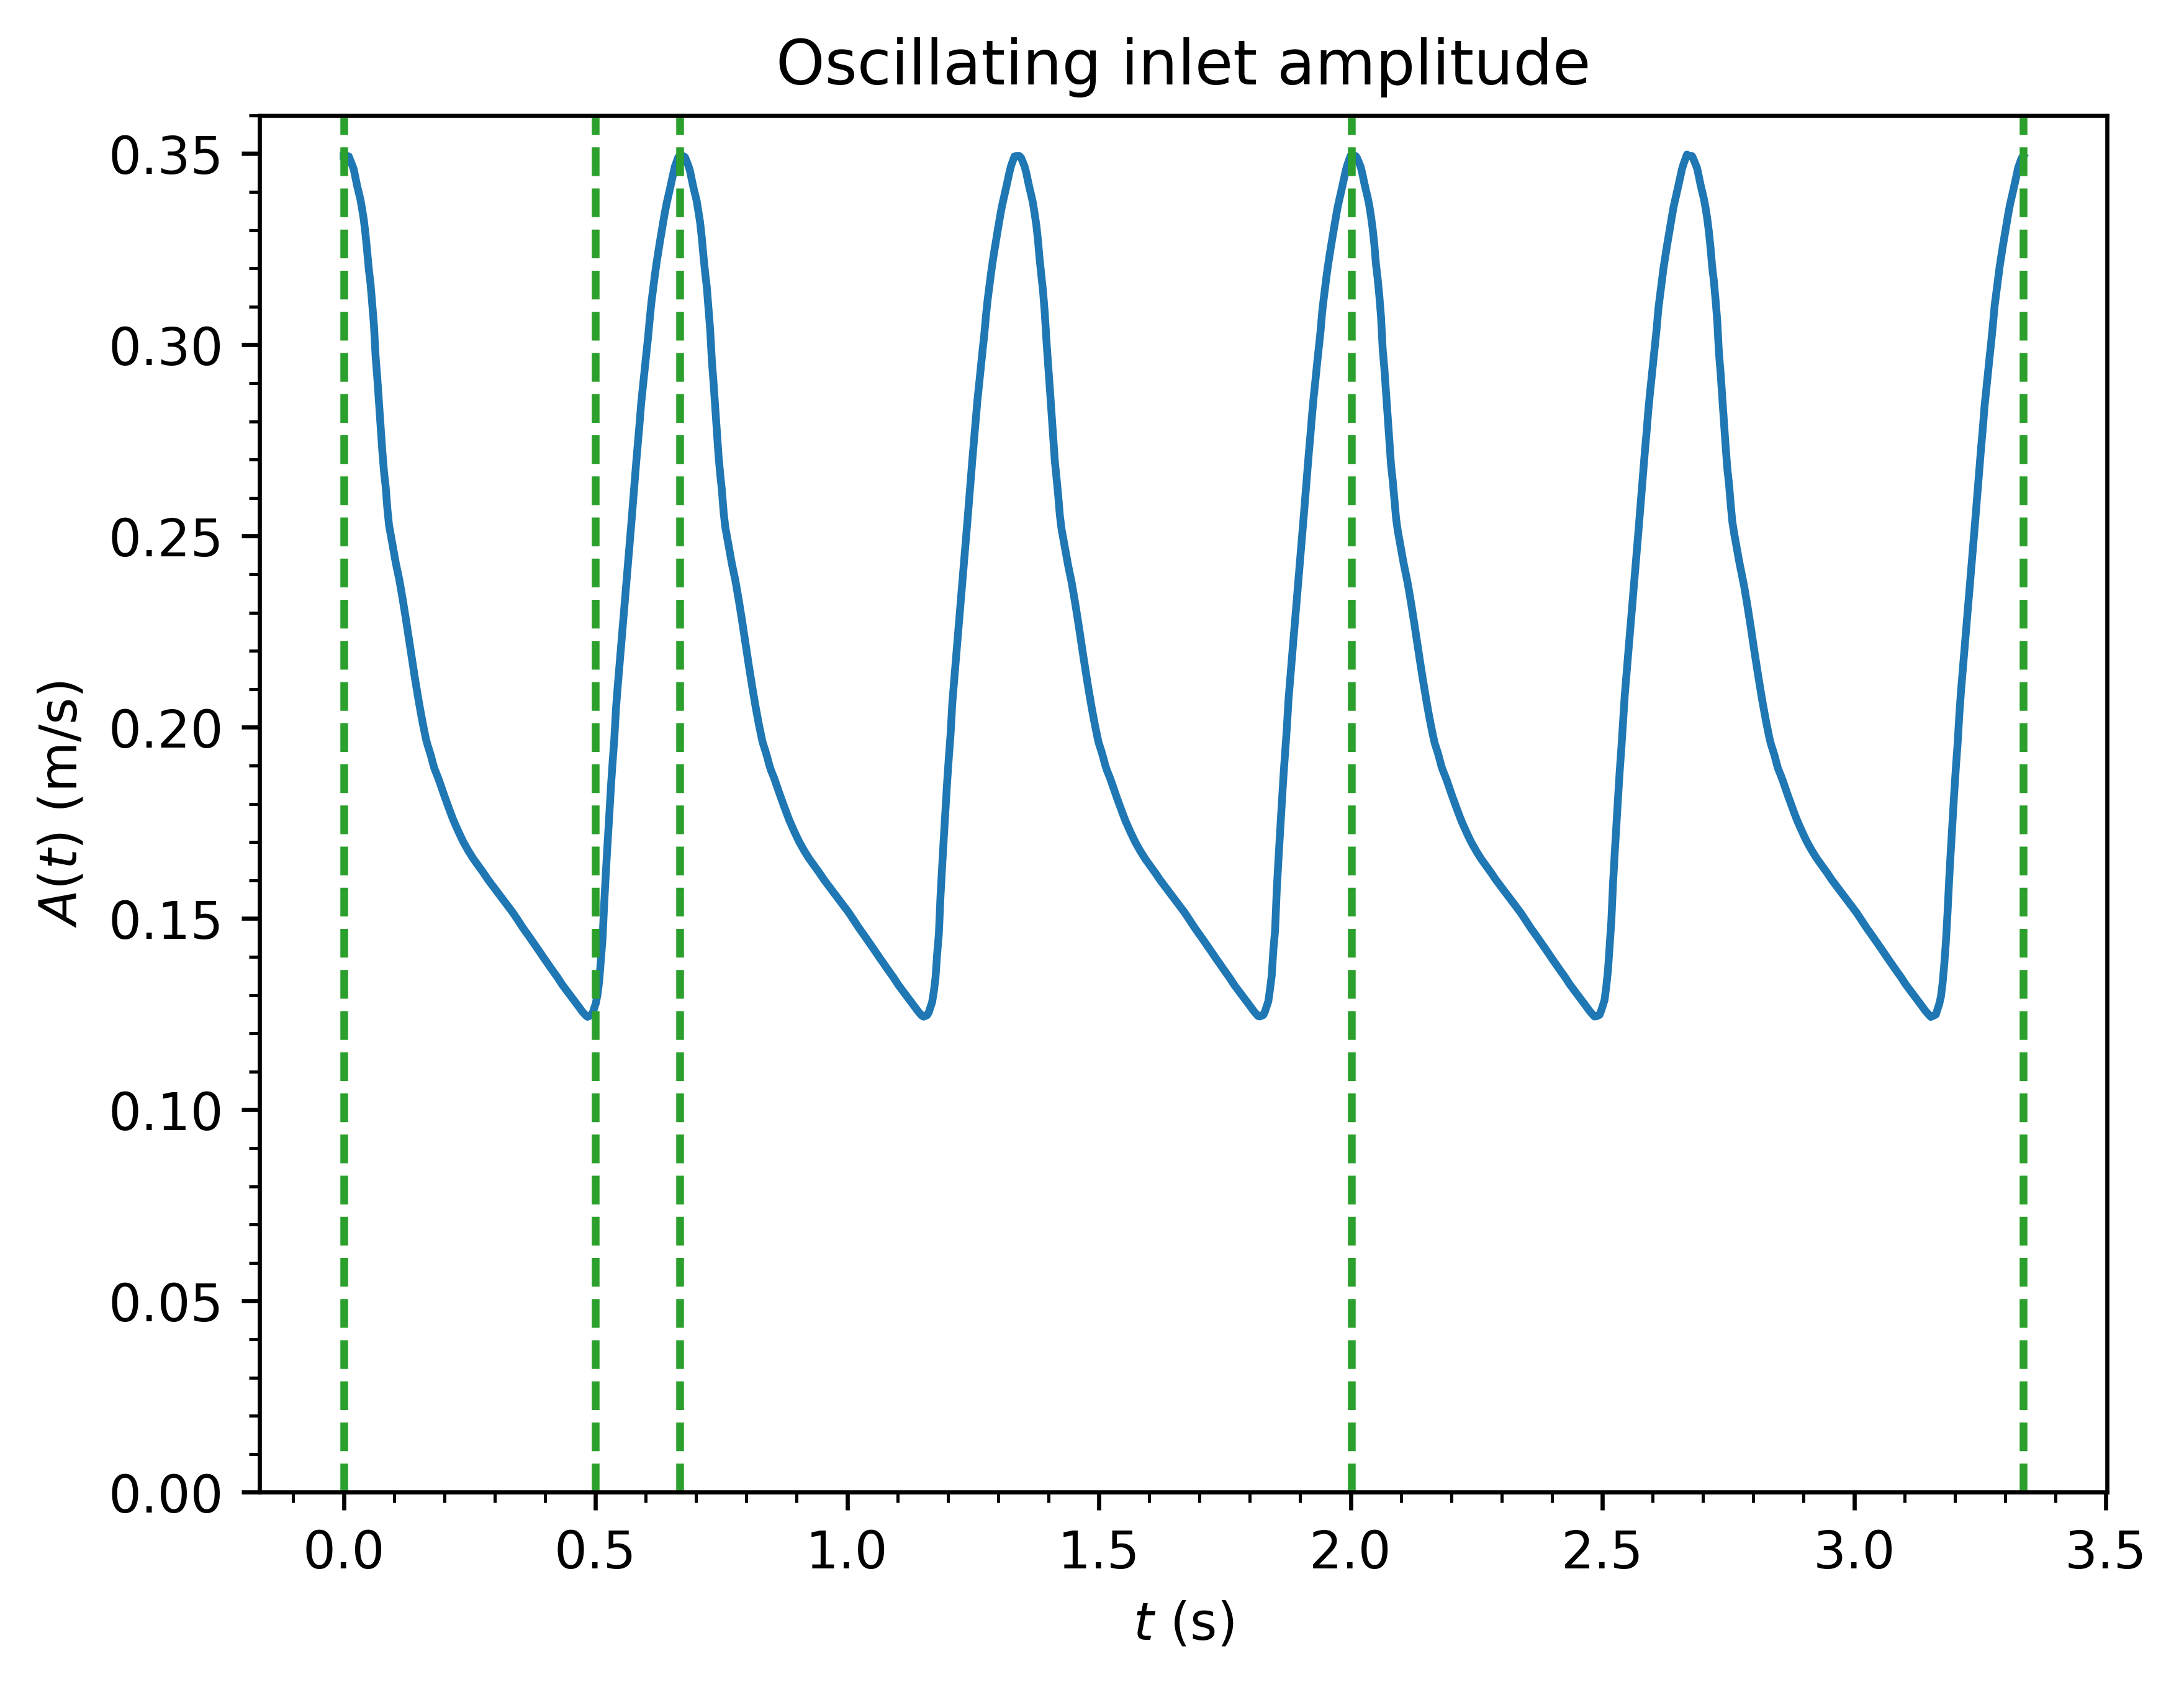
\includegraphics[width=0.6\textwidth]{diagrams/results-modelling/velocity-transport-oscillating/amplitude.png}
            \caption{Amplitude of the Poiseuille flow in \S\ref{sec:numerical-methods:time-dependent-experiments} that uses data from Figure 4(H) of \cite{carsonPersonalisingCardiovascularNetwork2021}. The profile presented here has been scaled such that the amplitude ranges between $A = \qty{0.12}{\metre\per\second}$ and $A = \qty{0.35}{\metre\per\second}$, and spans $t \in [0, T_N]$, which corresponds to five cardiac cycles with $T_N = 3.34$. Five green vertical lines correspond to times $t=0$, $t=0.500$, $t=0.667$, $t=2.002$, and $t=3.336$, and correspond to the five snapshots in time of the flow and oxygen concentration fields visualised in Figures \ref{fig:oscillating-inlet-velocity:1}--\ref{fig:oscillating-inlet-velocity:5} and \ref{fig:oscillating-inlet-transport:1}--\ref{fig:oscillating-inlet-transport:5}.}
            \label{fig:oscillating-inlet-amplitude}
        \end{figure}

        We will consider only five snapshots in time in the body of this thesis for ease of presentation. Videos visualising these fields through time at every time-step are available here\footnote{Velocity field: \url{https://r.blakey.family/phd-video-oiv}; oxygen concentration field: \url{https://r.blakey.family/phd-video-oit}.}. Figures \ref{fig:oscillating-inlet-velocity} and \ref{fig:oscillating-inlet-transport} respectively present snapshots of blood flow and oxygen concentration fields at the five discrete snapshots in time. Note that each snapshot is indicated in Figure \ref{fig:oscillating-inlet-amplitude} with green vertical lines. Panel (a) of Figures \ref{fig:oscillating-inlet-velocity} and \ref{fig:oscillating-inlet-transport} give the initial steady-state fields of the flow and oxygen concentration, respectively; we remark that these are identical to the fields presented in Figures \ref{fig:asymmetric-placenta} and \ref{fig:transport-placenta}, respectively. Panel (b) gives the fields at the first local minimum of the amplitude profile. Panels (c), (d), and (e) respectively give the fields at the second, fourth and sixth (and final) local maxima of the amplitude profile. We remark that the precise trajectories of each of the streamlines differs between each snapshot due to the flow field changing through time.

        It is not surprising that Figures \ref{fig:oscillating-inlet-velocity:1} and \ref{fig:oscillating-inlet-velocity:3}--\ref{fig:oscillating-inlet-velocity:5} are very similar, given that they all correspond to peaks in amplitude of the inlet velocity. However, a notable feature that changes between these snapshots is that the recirculation zones in all the placentones have disappeared by $t = T_N$, as shown in Figure \ref{fig:oscillating-inlet-velocity:5}. This is likely due to numerical dissipation of the time discretisation, which `smooths out' the flow as time progresses. Figure \ref{fig:oscillating-inlet-velocity:2} is a little different to the others, due to the reduced inlet speed here; overall, the flow field exhibits very similar behaviour, but the flow is slower in most areas of the domain. 

        \begin{figure}
            \centering
            \begin{subfigure}{\textwidth}
                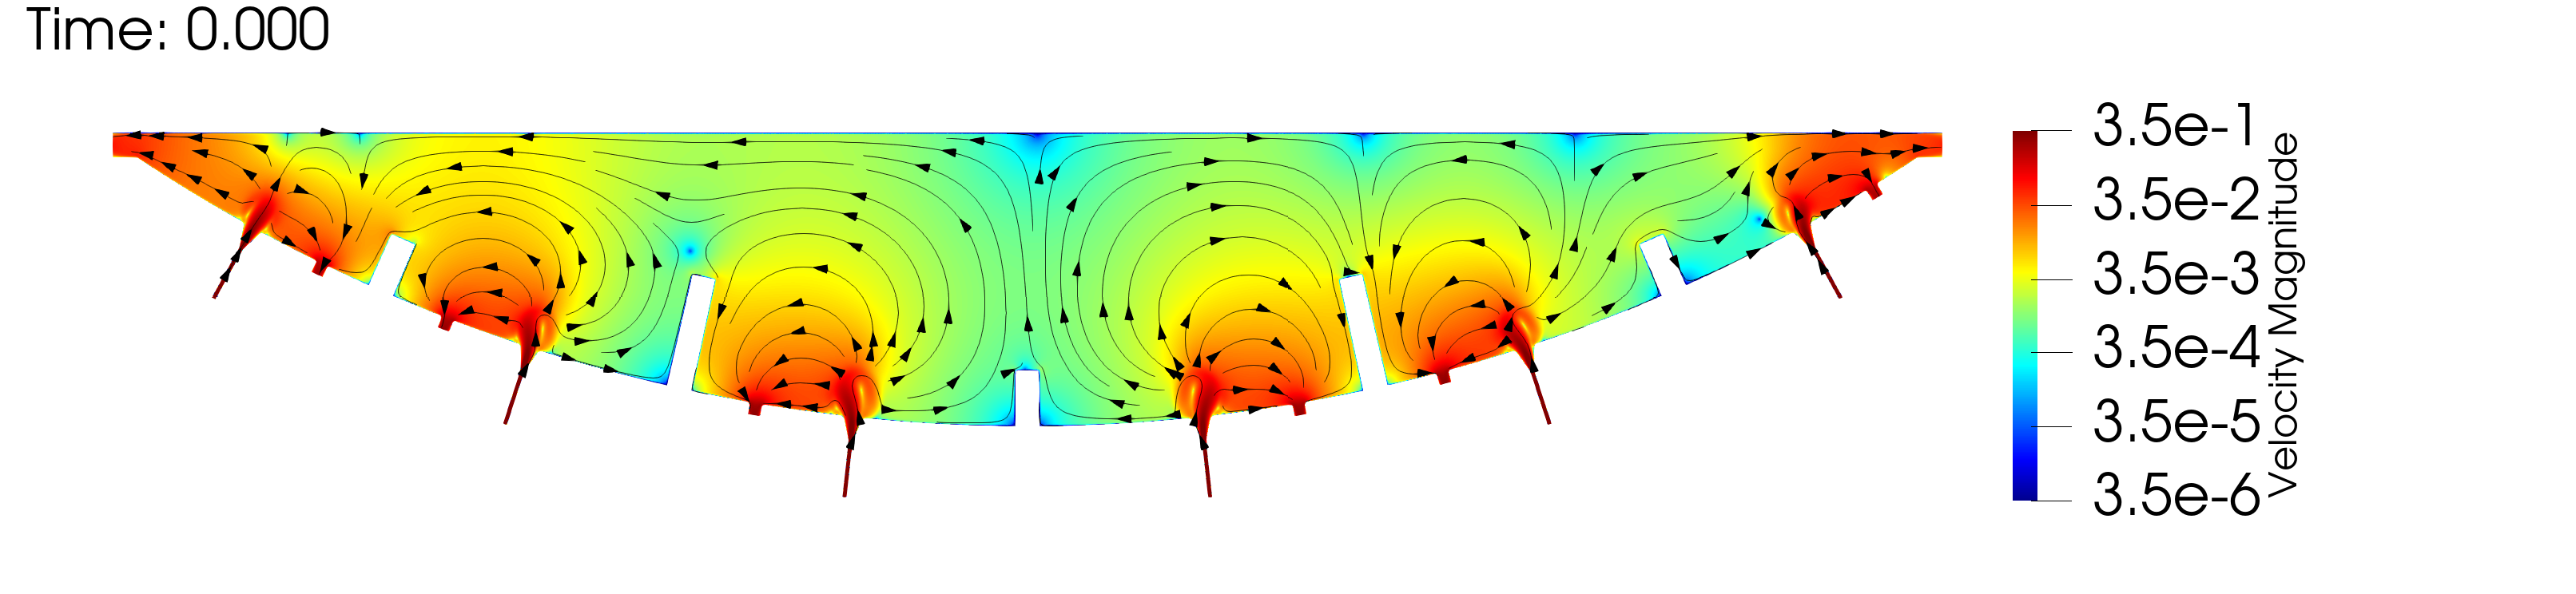
\includegraphics[width=\textwidth]{diagrams/results-modelling/velocity-transport-oscillating/placenta-velocity/velocity.0000.png}
                \caption{}
                \label{fig:oscillating-inlet-velocity:1}
            \end{subfigure}
            \begin{subfigure}{\textwidth}
                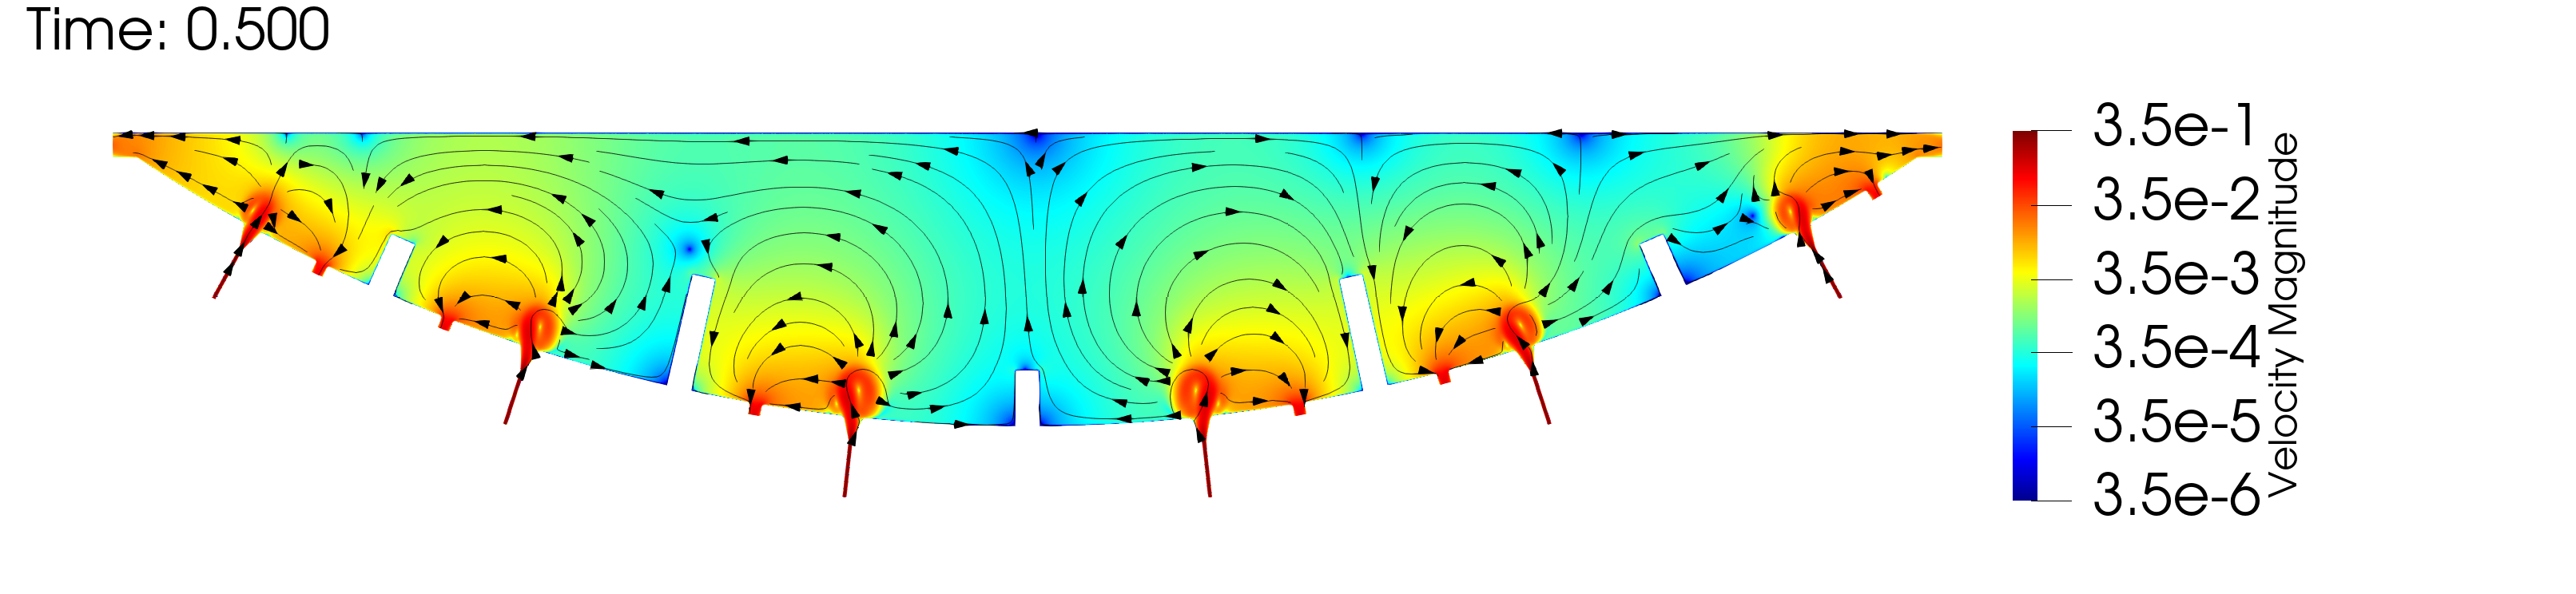
\includegraphics[width=\textwidth]{diagrams/results-modelling/velocity-transport-oscillating/placenta-velocity/velocity.0015.png}
                \caption{}
                \label{fig:oscillating-inlet-velocity:2}
            \end{subfigure}
            \begin{subfigure}{\textwidth}
                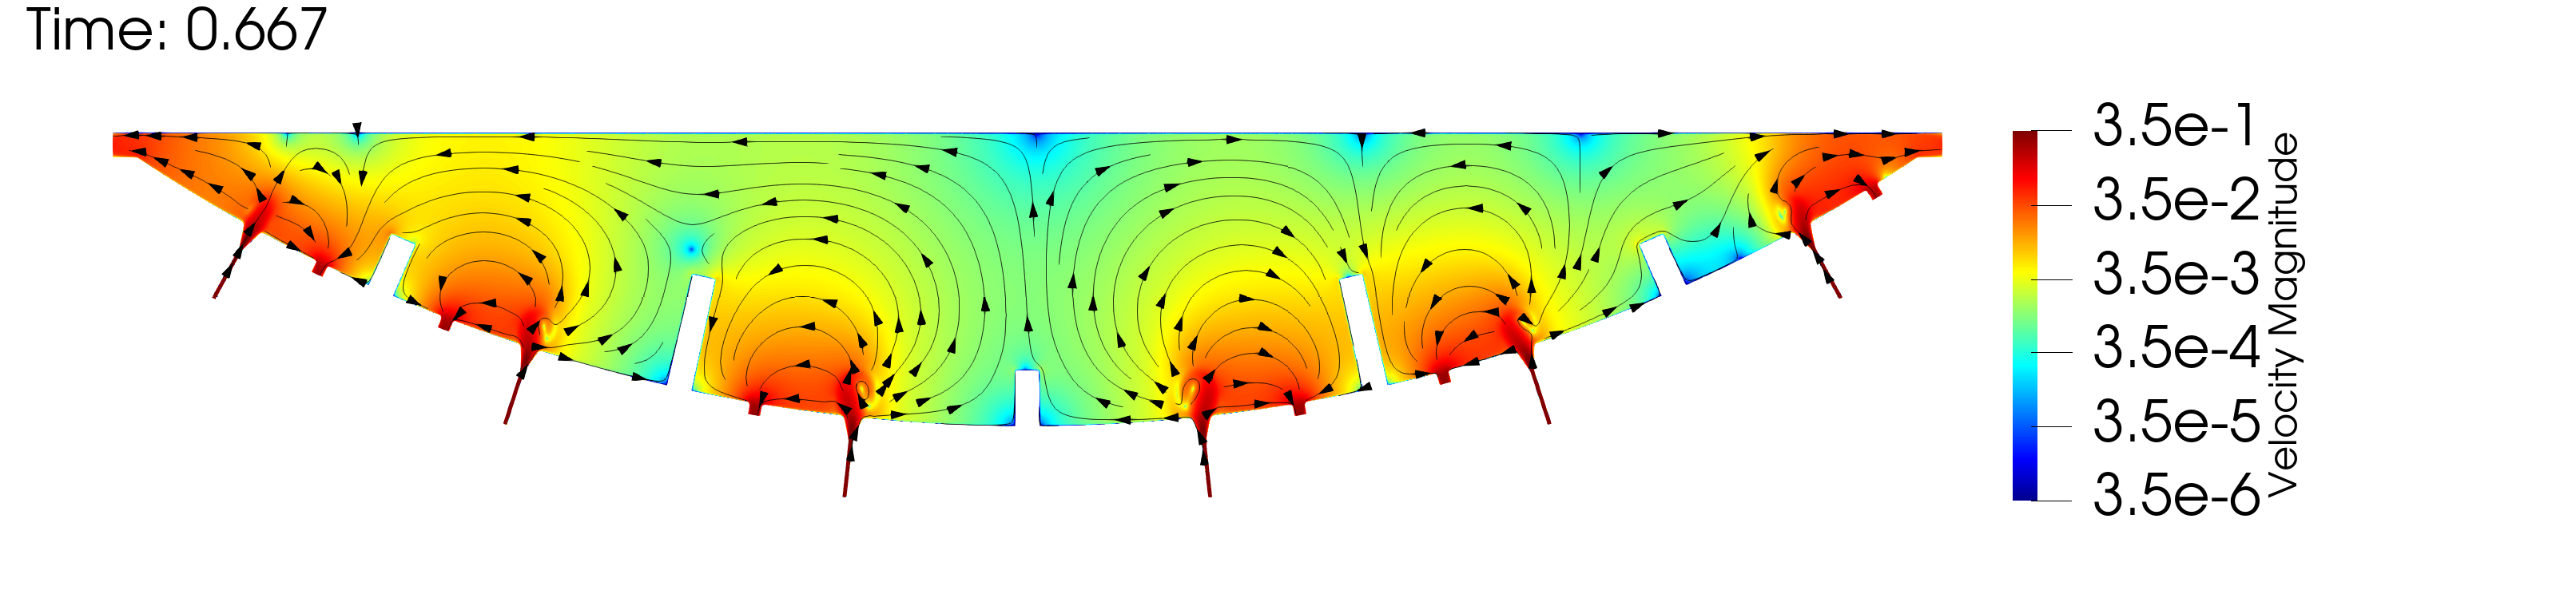
\includegraphics[width=\textwidth]{diagrams/results-modelling/velocity-transport-oscillating/placenta-velocity/velocity.0020.png}
                \caption{}
                \label{fig:oscillating-inlet-velocity:3}
            \end{subfigure}
            \begin{subfigure}{\textwidth}
                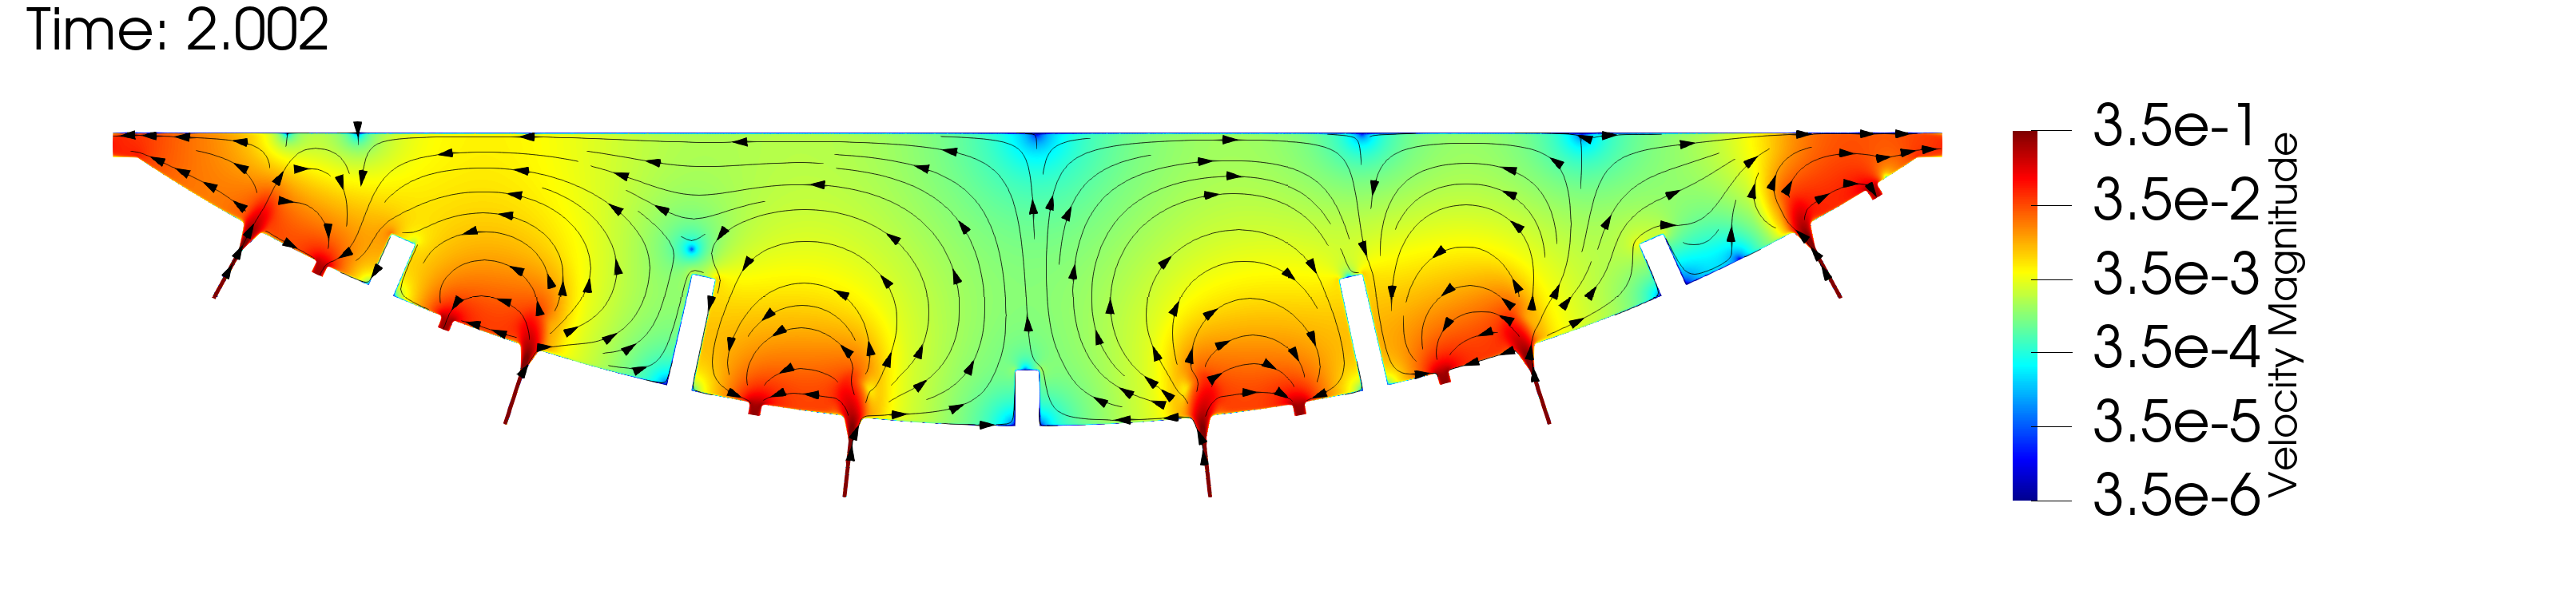
\includegraphics[width=\textwidth]{diagrams/results-modelling/velocity-transport-oscillating/placenta-velocity/velocity.0060.png}
                \caption{}
                \label{fig:oscillating-inlet-velocity:4}
            \end{subfigure}
            \begin{subfigure}{\textwidth}
                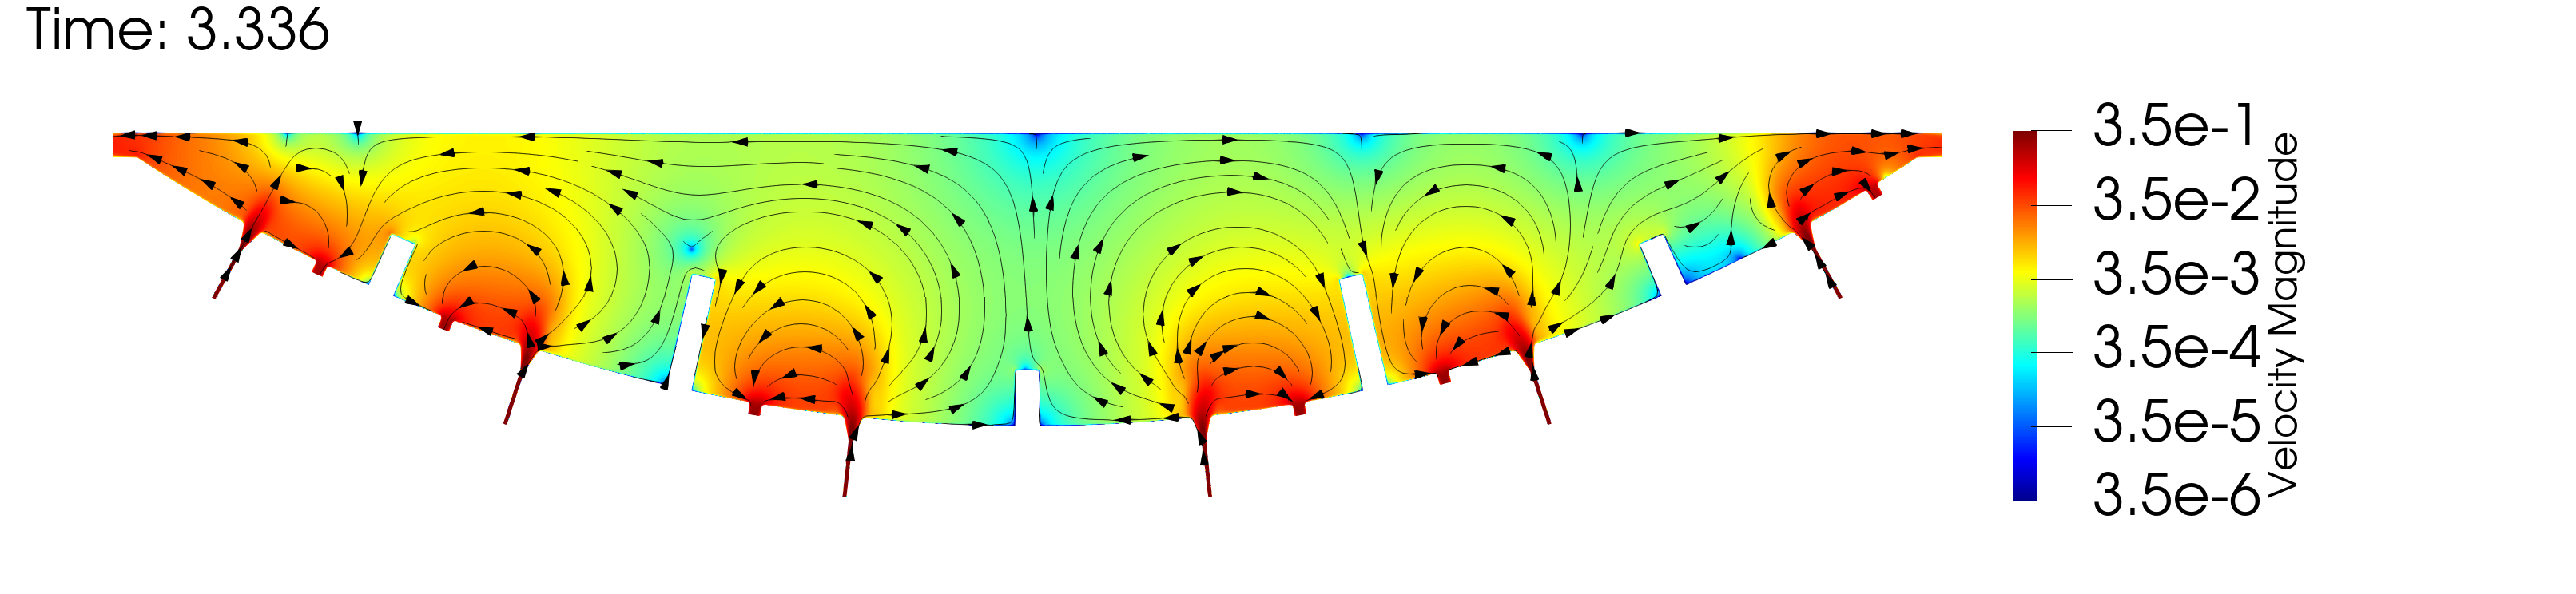
\includegraphics[width=\textwidth]{diagrams/results-modelling/velocity-transport-oscillating/placenta-velocity/velocity.0100.png}
                \caption{}
                \label{fig:oscillating-inlet-velocity:5}
            \end{subfigure}
            \caption{Visualisation of the blood flow field (Equation \eqref{eq:nsb}) with a pulsatile inflow condition in \S\ref{sec:numerical-methods:time-dependent-experiments} at times (a) $t=0$, (b) $t=0.500$, (c) $t=0.667$, (d) $t=2.002$, and (e) $t=3.336$. Colours are logarithmically scaled, and streamlines at each time-step are shown with black lines. A video visualising all time-steps can be viewed here: \url{https://r.blakey.family/phd-video-oiv}}
            \label{fig:oscillating-inlet-velocity}
        \end{figure}

        \begin{figure}
            \thisfloatpagestyle{empty}
            \centering
            \begin{subfigure}{\textwidth}
                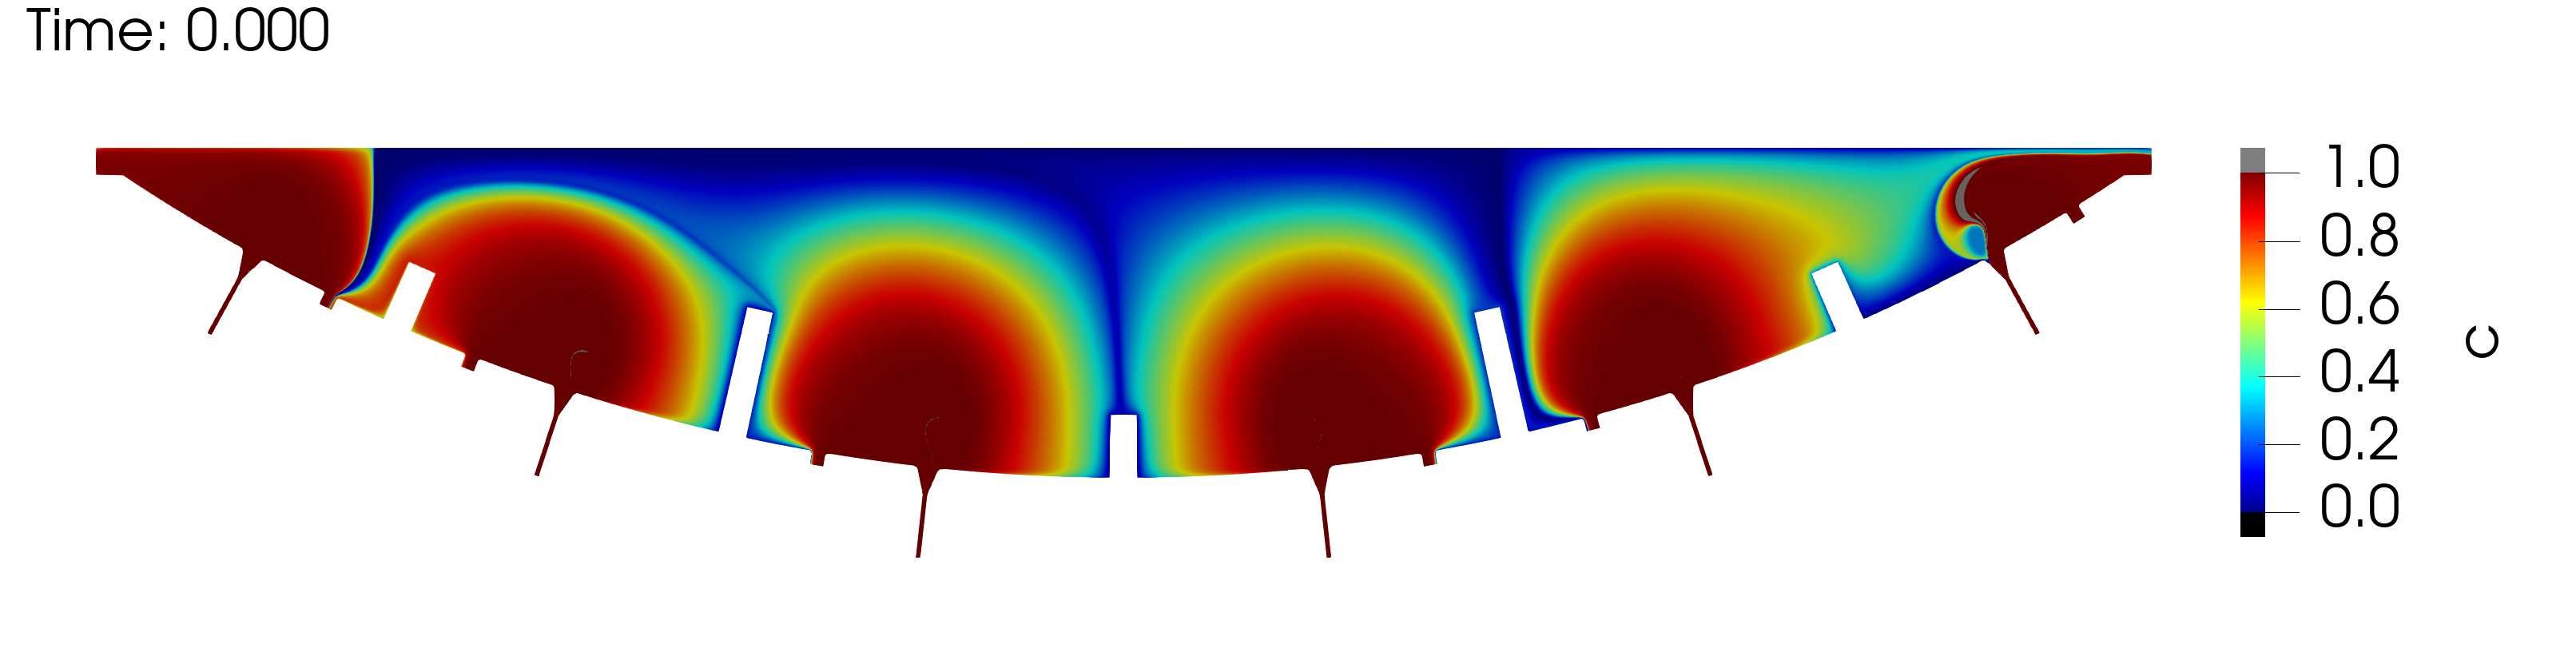
\includegraphics[width=\textwidth]{diagrams/results-modelling/velocity-transport-oscillating/placenta-transport/transport.0000.png}
                \caption{}
                \label{fig:oscillating-inlet-transport:1}
            \end{subfigure}
            \begin{subfigure}{\textwidth}
                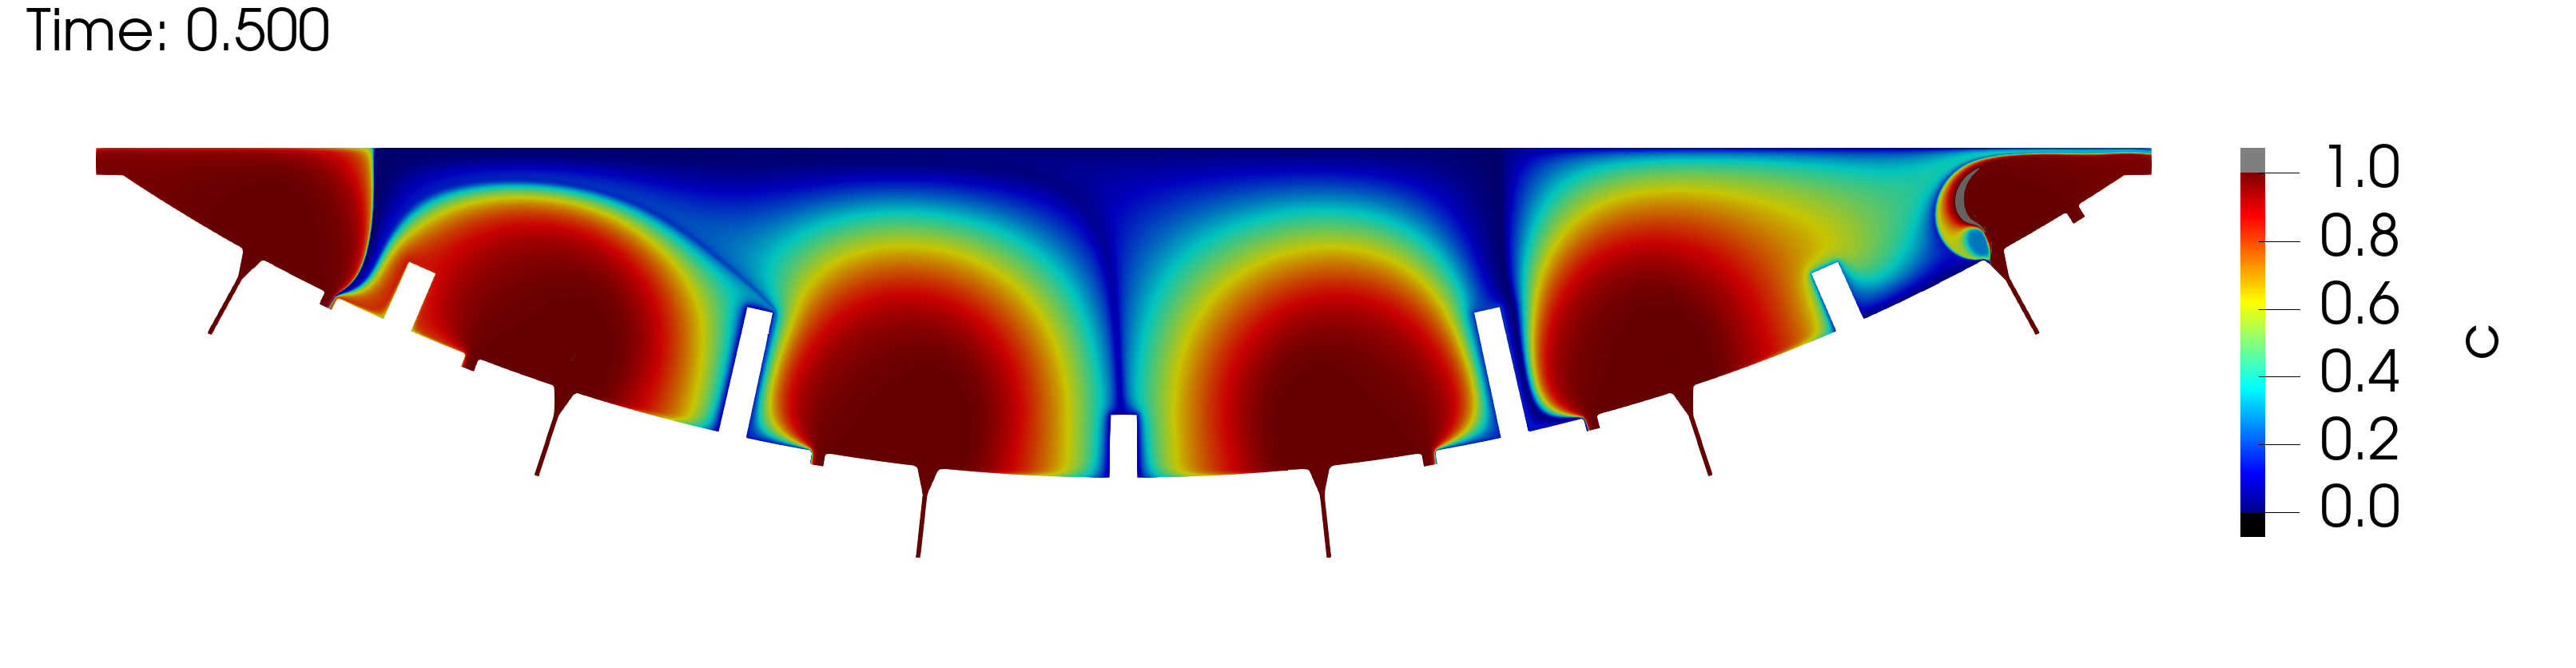
\includegraphics[width=\textwidth]{diagrams/results-modelling/velocity-transport-oscillating/placenta-transport/transport.0015.png}
                \caption{}
                \label{fig:oscillating-inlet-transport:2}
            \end{subfigure}
            \begin{subfigure}{\textwidth}
                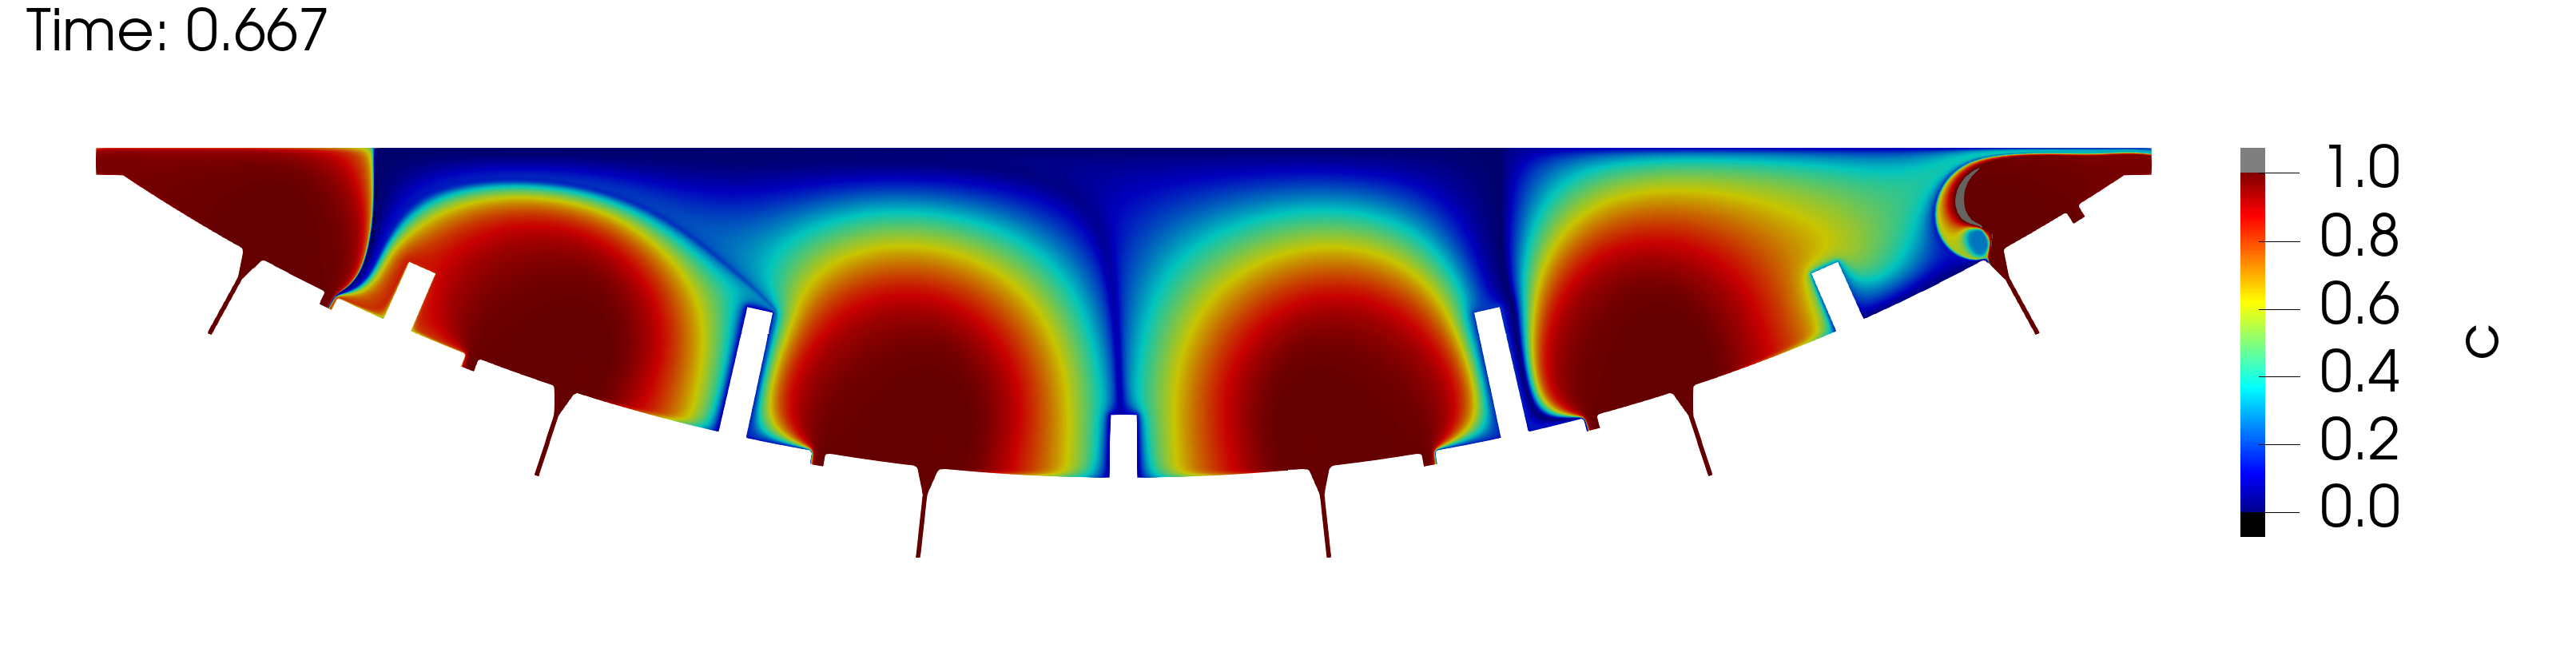
\includegraphics[width=\textwidth]{diagrams/results-modelling/velocity-transport-oscillating/placenta-transport/transport.0020.png}
                \caption{}
                \label{fig:oscillating-inlet-transport:3}
            \end{subfigure}
            \begin{subfigure}{\textwidth}
                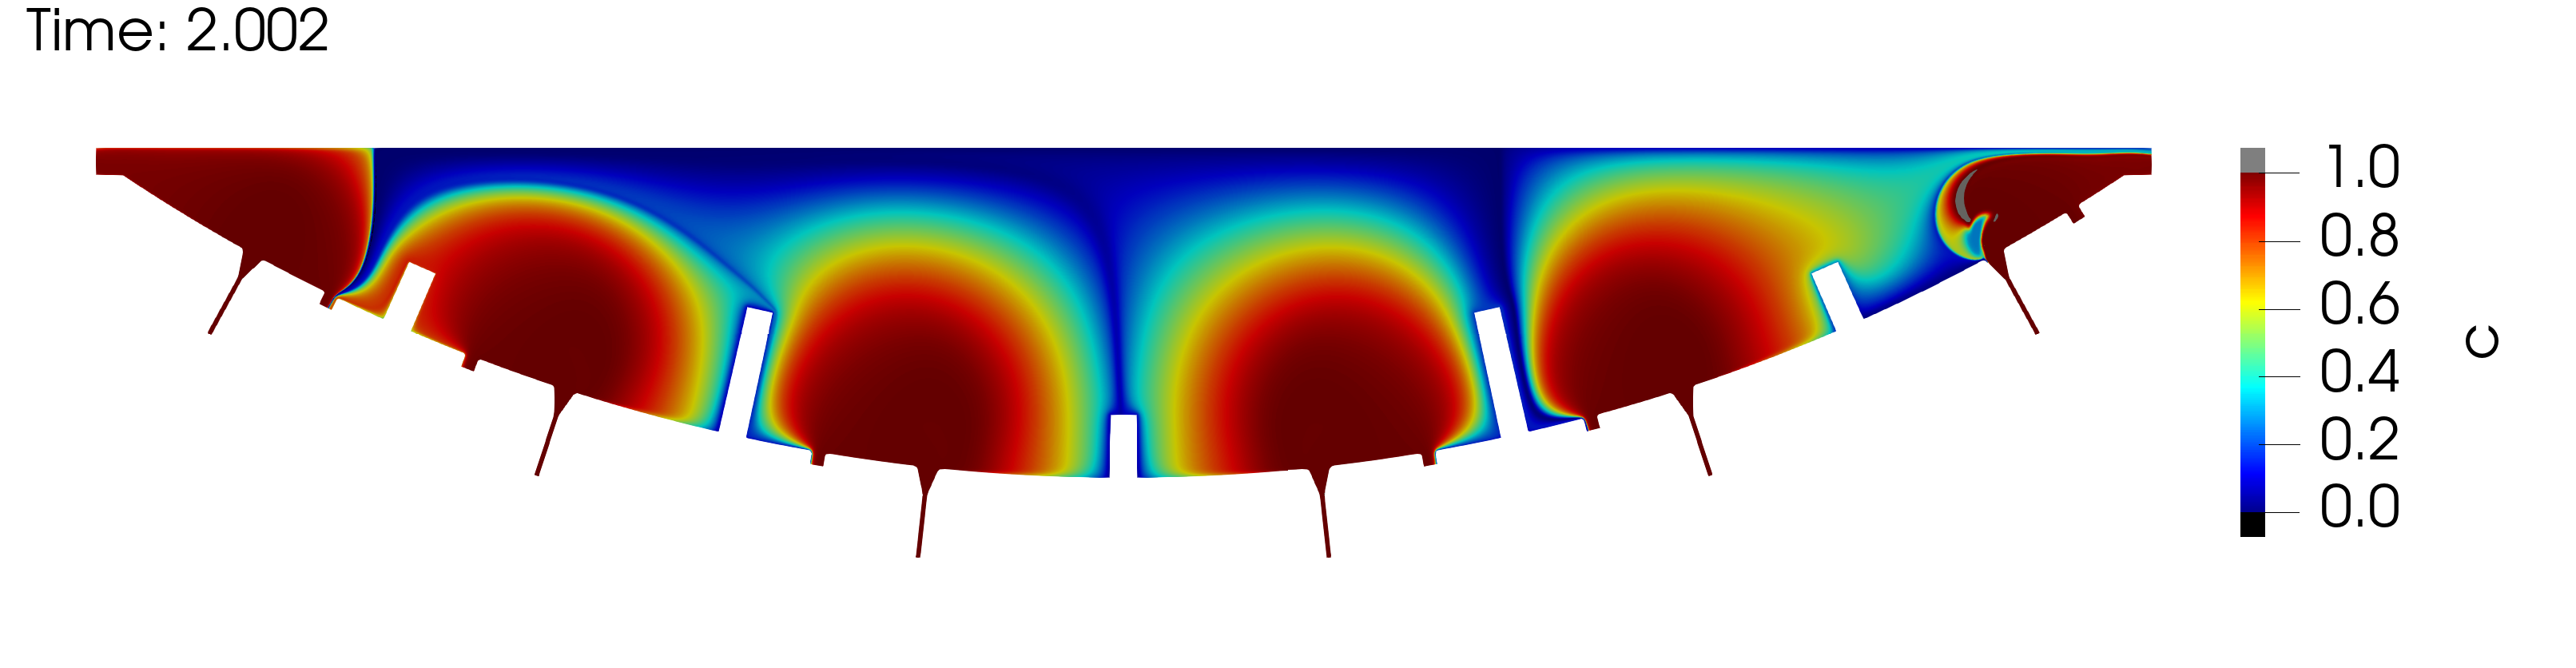
\includegraphics[width=\textwidth]{diagrams/results-modelling/velocity-transport-oscillating/placenta-transport/transport.0060.png}
                \caption{}
                \label{fig:oscillating-inlet-transport:4}
            \end{subfigure}
            \begin{subfigure}{\textwidth}
                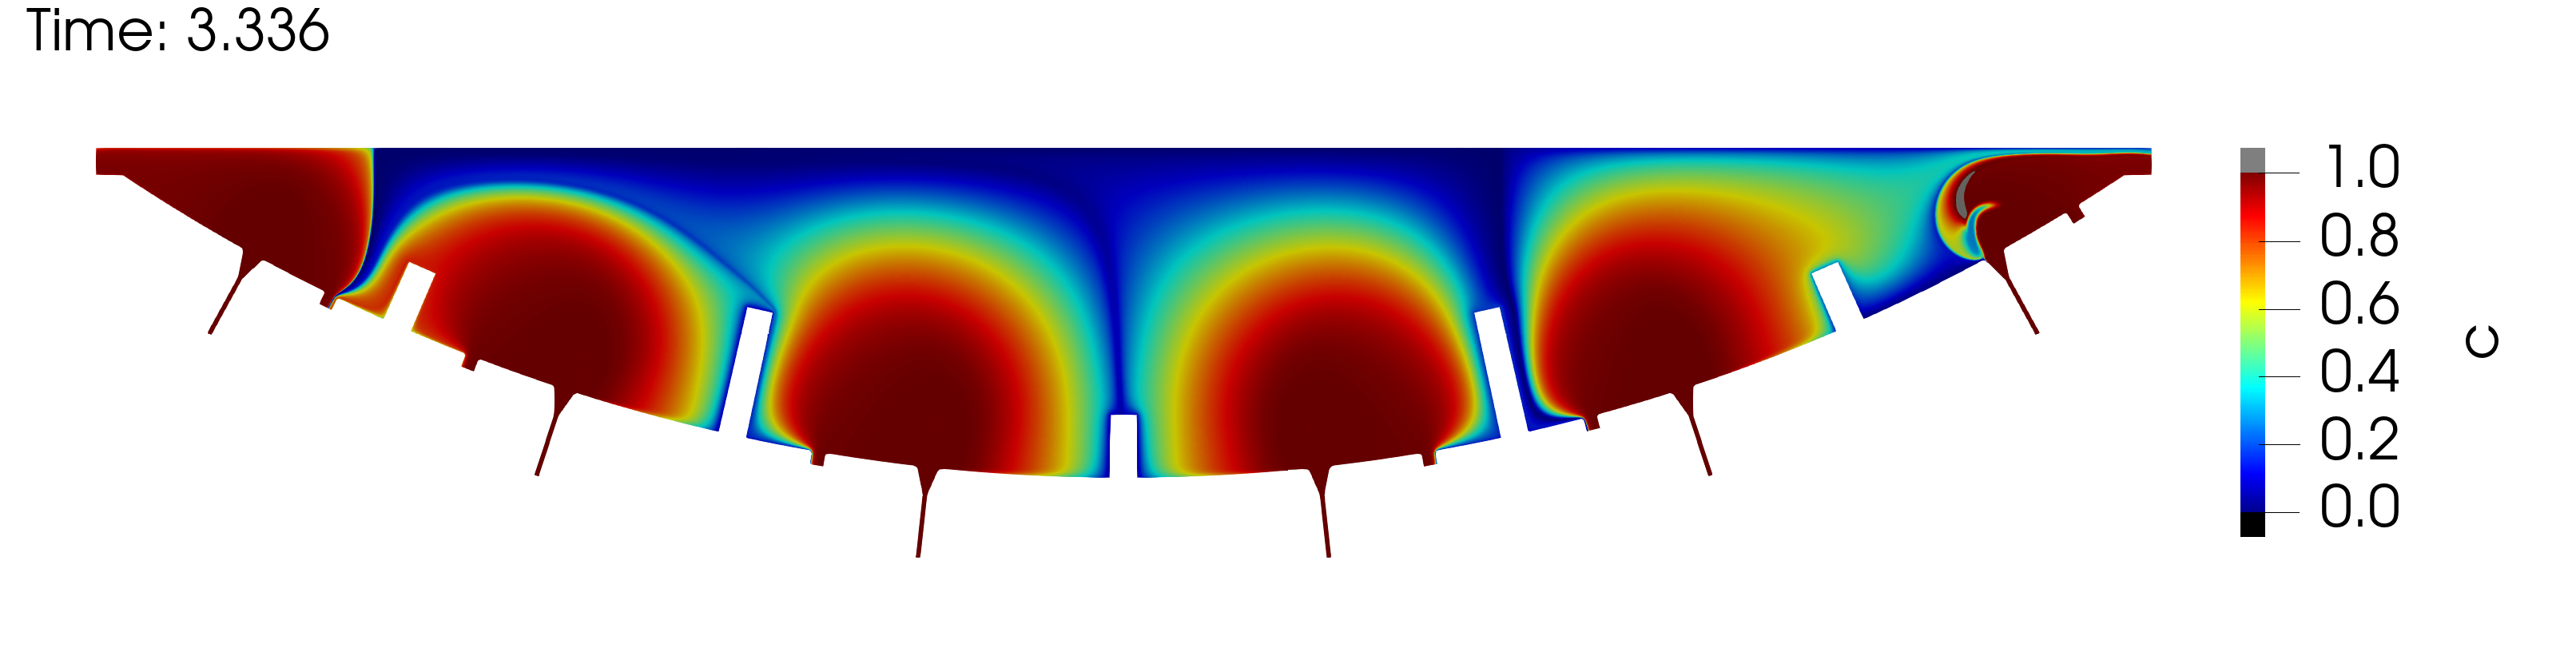
\includegraphics[width=\textwidth]{diagrams/results-modelling/velocity-transport-oscillating/placenta-transport/transport.0100.png}
                \caption{}
                \label{fig:oscillating-inlet-transport:5}
            \end{subfigure}
            \caption{Visualisation of the oxygen concentration field (Equation \eqref{eq:rad}) with a pulsatile inflow condition in \S\ref{sec:numerical-methods:time-dependent-experiments} at times (a) $t=0$, (b) $t=0.500$, (c) $t=0.667$, (d) $t=2.002$, and (e) $t=3.336$. Colours are linearly scaled. A video visualising all time-steps can be viewed here: \url{https://r.blakey.family/phd-video-oit}}
            \label{fig:oscillating-inlet-transport}
        \end{figure}

        The most intriguing feature of these results is that, although the speed of the flow noticeably changes with lower amplitude in Figure \ref{fig:oscillating-inlet-velocity:2}, there is almost no perceivable change in the oxygen concentration field across all time-steps. This is primarily due to $|\vec{u}| \ll \qty{1e-1}{\metre\per\second}$ everywhere except in the central cavity, arteries, and veins; we therefore only expect changes in $c$ in these areas of relatively fast flow on this timescale. However, almost all of the placentones have $c \approx 1$ uniformly in these fast flow regions. An exception in this particular simulation is in the furthest-right placentone, where there is a small recirculation zone of low concentration beside the artery mouth, which arises from the initial condition. As time progresses, the evolution of the velocity field moves the recirculation zone, therefore advecting with non-zero speed the low concentrations of oxygen in this recirculation zone. This effect eventually draws low concentrations of oxygen away from the recirculation zone into the IVS and towards the marginal sinus. We highlight that this behaviour is due to the initial condition of this particular problem, and is unlikely to be relevant to more general situations with a similar setup.

        In summary, applying a pulsatile inlet flow that follows the cardiac cycle has very little effect on flow and oxygen concentration in the simulation we have presented. Whilst there may be other situations where pulsatile inlet flow has a more discernable effect on oxygen transport, most of the remaining simulations in this thesis will consider only steady-state flow and transport at peak systole, except for Chapter \ref{sec:contractions} where time dependence is imposed through boundary motion.
        
        We will now conclude this chapter with a summary of what has been presented and how these discretisations will be used throughout the remainder of the thesis.        

    \section{Summary} \label{sec:numerical-methods:summary}
        In Chapter \ref{sec:numerical-methods}, we have introduced a DGFEM discretisation of the models of maternal blood flow and oxygen transport from Chapter \ref{sec:modelling}, including a convergence study and some basic numerical experiments on the steady-state versions of these models, which included a comparison between our choice of blood flow model with two related choices. We also briefly presented a numerical experiment of the time-dependent version of NSD and the oxygen-transport model.

        \S\ref{sec:numerical-methods:dgfem} began by introducing the finite element spaces in which the approximate solutions are sought. \S\ref{sec:numerical-methods:equation-discretisations} then introduced the full equation discretisations, where spatial derivatives have been discretised using a DGFEM, and temporal derivatives have been discretised using a backward Euler finite difference approximation. We chose a Lax-Friedrichs flux to approximate the advective terms on element faces, which is a form of upwind flux.

        Next, \S\ref{sec:numerical-methods:convergence} used the method of manufactured solution (MMS) to investigate the convergence rates of the time-dependent versions of the blood flow and oxygen transport models. We found that we achieved optimal spatial and temporal convergence rates for the finite element spaces and time discretisation method we have used. However, a limitation of our time discretisation is that it is only first-order accurate, which in practice limits us to a choice of small time-step. Whilst backward Euler is unconditionally stable, an obvious improvement in terms of accuracy would be to employ a time discretisation scheme from, e.g., the Runge-Kutta family, where higher-order discretisations are available.

        We then performed several blood flow numerical experiments. Firstly, \S\ref{sec:numerical-methods:blood-flow-experiments} presented example blood flows on both the placentone and placenta geometries for NSD and the two related velocity models for the parameters outlined in Tables \ref{tab:structural-parameters} and \ref{tab:problem-parameters}. We showed that NSD displays roughly the same behaviour in the IVS of the other two alternative velocity models, with some notable differences in the CC, and the advantage that it gives a physiologically sensible transition region between `free' and porous flow. We also presented a numerical experiment on the placenta geometry where veins are placed asymmetrically in \S\ref{sec:numerical-methods:blood-flow-experiments:asymmetric}. In this example, we found that high-speed flow remained close to the basal plate, but increased flow speed by an order of magnitude in the region closest to the chorionic plate. This asymmetric experiment is important, as it introduces asymmetries that would be typical in a physical placenta; this experiment therefore forms the basis of the investigations in Chapters \ref{sec:numerical-mri} and \ref{sec:contractions}.
        
        Next, \S\ref{sec:numerical-methods:nutrient-transport-experiments} presented the distribution of oxygen concentration on the asymmetric placenta geometry, where the underlying advective flow is governed by NSD. Overall, the oxygen concentration perfuses radially from the spiral artery, which agrees with the results of \citeauthor{chernyavskyMathematicalModelIntervillous2010} \cite{chernyavskyMathematicalModelIntervillous2010}. Interestingly, oxygen was found to exit the placenta in high concentration; this is oxygen that could be uptaken by the villous tree given the right conditions, and will be investigated further in Chapter \ref{sec:nutrient-uptake}.
        
        Finally, \S\ref{sec:numerical-methods:time-dependent-experiments} presented a time-dependent blood flow and oxygen numerical experiment, where the time-dependence was driven by a pulsatile inflow arising from the cardiac cycle. We found that the pulsatile inflow had very little effect on the oxygen concentration field, due to the high concentration of oxygen near the spiral artery. The analyses of Chapters \ref{sec:nutrient-uptake} and \ref{sec:numerical-mri} will consider only steady-state flow, but Chapter \ref{sec:contractions} will introduce time-dependent flow that is imposed through boundary motion.

        An obvious extension to the work in this thesis would be to consider maternal flow in 3D, rather than the 2D description we have adopted. Other studies do consider maternal flow in 3D (e.g., \cite{chernyavskyMathematicalModelIntervillous2010,meklerImpactTissuePorosity2022}), but rely on several strong assumptions, such as symmetry of vessels or simplifications to the geometry. This is not the case for the asymmetric results presented here in 2D, with the symmetry assumptions relaxed further in Chapter \ref{sec:nutrient-uptake}. Considering flow in 2D in this thesis also allows for a more feasible computational study than an equivalent 3D study. As far as we are aware, there is no published work that tackles 3D maternal flow in such a general computational framework. However, work such as \citeauthor{crowsonInvestigatingPlacentalHemodynamics2024} \cite{crowsonInvestigatingPlacentalHemodynamics2024} is likely to be an exciting development, where an organ-scale 3D geometry of the placenta is used to determine how structural variations affect placental function.

        The following three chapters of this thesis now develop in three different ways: Chapter \ref{sec:nutrient-uptake} will vary structural parameters to study effects on placental efficiency; Chapter \ref{sec:numerical-mri} will artificially recreate MRI data for direct comparison between simulated and physical placental flow fields; and Chapter \ref{sec:contractions} will introduce a preliminary contraction model of the utero-placental pump.